\documentclass[a4paper]{article}
\usepackage{html}
\usepackage{graphicx}
%\usepackage{hyperref}
\usepackage{amssymb,amsmath}
\newcommand{\oofem}{\htmladdnormallink{OOFEM}{http://www.oofem.org}\ }
\newcommand{\bp}{\htmladdnormallink{Bo\v{r}ek Patz\'{a}k}{http://mech.fsv.cvut.cz/~bp/bp.html}}

\renewcommand{\topfraction}{0.99}    % 99% of page top can be a float
\renewcommand{\bottomfraction}{0.99}    % 99% of page bottom can be a float
\renewcommand{\textfraction}{0.01}    % only 1% of page must to be the text
\renewcommand{\floatpagefraction}{0.99} % 99% of whole page can be a float
\setcounter{totalnumber}{5} %maximum floating objects on one page

\newcommand{\mbf}[1]{\mbox{\boldmath$#1$}}
\newcommand{\descitem}[1]{{\noindent \bf #1}}
\newcommand{\elemkeyword}[1]{\descitem{Keyword}~{\em #1}}
\newcommand{\elemparam}[2]{{{#1\tiny (#2)}~\#}}
\newcommand{\optelemparam}[2]{[{~\elemparam{#1}{#2}}]}
\newcommand{\param}[1]{{\it #1}}
\newcommand{\optparam}[1]{[{\it #1}]}
\newcommand{\be}{\begin{equation}}
\newcommand{\ee}{\end{equation}}
\newcommand{\bea}{\begin{eqnarray}}
\newcommand{\eea}{\end{eqnarray}}
\newcommand{\bsig}{\mbf{\sigma}}
\newcommand{\alphaPsi}{\alpha_{\psi}}
\newcommand{\kappac}{\kappa_{\mathrm{c}}}
\newcommand{\tauY}{\tau_{\mathrm {Y}}}
\newcommand{\eps} {\mbf{\varepsilon}}
\newcommand{\epss} {\varepsilon}%scalar
\newcommand{\epsp} {\eps_{\mathrm{p}}}
\newcommand{\epspd} {\dot{\eps}_{\mathrm{p}}}
\newcommand{\ignore}[1]{}
\newcommand{\del}[2]{\mbox{$\displaystyle\frac{#1}{#2}$}}
\newcommand{\ep}[0]{\mbf{\varepsilon}^p}
\newcommand{\epd}[0]{\dot{\mbf{\varepsilon}}^p}
\newcommand{\e}{\mbf{\varepsilon}}
\newcommand{\sig}{\mbf{\sigma}}
\newcommand{\sigs}{\sigma}%scalar
\newcommand{\kap}{\mbf{\kappa}}
\newcommand{\ve}{\mbf{e}}% vector e
\newcommand{\vet}{\tilde{\ve}}
\newcommand{\veps}{\mbf{\varepsilon}}  % vector epsilon
\newcommand{\vsig}{\mbf{\sigma}}% vector sigma
\newcommand{\vs}{\mbf{s}}% vector s
\newcommand{\vepst}{\tilde{\veps}}
\newcommand{\vst}{\mbf{s}^T}% vector s transposed
\newcommand{\vsigt}{\tilde{\vsig}}
\newcommand{\dvepst}{\delta\tilde{\veps}}
\newcommand{\dvet}{\delta\vet}
\newcommand{\dvs}{\delta\vs}
\newcommand{\dvsig}{\delta\vsig}
\newcommand{\dO}{\,\mbox{d}\Omega}
\newcommand{\ud}{\mathrm{d}}
\newcommand{\sym}{_{\mbox{\small sym}}}
\newcommand{\vxi}{\mbf{\xi}}% vector xi
\newcommand{\quarter}{\mbox{$\frac{1}{4}$}}
\newcommand{\vx}{\mbf{x}}% vector x
\newcommand{\refeq}[1]{Eq.~(\ref{#1})}
\newcommand{\reffig}[1]{Fig.~(\ref{#1})}
\newcommand{\refeqs}[2]{Eqs.~(\ref{#1}), (\ref{#2})}
\newcommand{\refeqsr}[2]{\mbox{Eqs.~(\ref{#1})-(\ref{#2})}}
\newcommand{\C}{$^{\circ}\mathrm{C}$}

\begin{document}


%begin{latexonly}
\title{
\oofemlnk{\centerline{
\includegraphics[width=0.7\textwidth]{oofem-logo-contour}}}
Material Model Library Manual}
\author{\bp \\ \\
Czech Technical University\\
Faculty of Civil Engineering\\
Department of Structural Mechanics\\
Th\'akurova 7, 166 29 Prague, Czech Republic
}
\maketitle
%end{latexonly}
\begin{htmlonly}
\begin{center}
\oofemlnk{\centerline{
\includegraphics[width=0.7\textwidth]{oofem-logo-contour.eps}}}
{\Large Material Model Library Manual}\\ \\
{\bp \\
Czech Technical University\\
Faculty of Civil Engineering\\
Department of Structural Mechanics\\
Th\'akurova 7, 166 29 Prague, Czech Republic
}
\end{htmlonly}

\newpage
\tableofcontents
\listoftables
\newpage
\section{Material Models for Structural Analysis}
\subsection{Elastic materials}
\subsubsection{Isotropic linear elastic material - IsoLE}
\label{IsoLE}
Linear isotropic material model. The model parameters are summarized
in Tab.~\ref{IsoLE_table}.

\begin{table}[!htb]
%\begin{center}
\begin{tabular}{|l|p{9cm}|}
\hline
Description & Linear isotropic elastic material\\
\hline
Record Format & \descitem{IsoLE} \elemparam{num}{in}
\elemparam{d}{rn} \elemparam{E}{rn} \elemparam{n}{rn}
\elemparam{tAlpha}{rn}\\
Parameters &- \param{num} material model number\\
&- \param{d} material density\\
&- \param{E} Young modulus\\
&- \param{n} Poisson ratio\\
&- \param{tAlpha} thermal dilatation coefficient\\
Supported modes& 3dMat, PlaneStress, PlaneStrain, 1dMat,
2dPlateLayer, 2dBeamLayer, 3dShellLayer, 2dPlate, 2dBeam, 3dShell,
3dBeam, PlaneStressRot\\
Features & Adaptivity support\\
\hline
\end{tabular}
\caption{Linear Isotropic Material - summary.}
\label{IsoLE_table}
%\end{center}
\end{table}



\subsubsection{Orthotropic linear elastic material - OrthoLE}
\label{OrthoLE}
Linear orthotropic, linear elastic  material model. The model parameters are summarized
in Tab.~\ref{OrthoLE_table}.
Local coordinate system, which determines axes of material orthotrophy
can by specified using \param{lcs} array. This array contains six numbers,
where the first three numbers represent directional vector of a local x-axis,
and next three numbers represent directional vector of a local y-axis.
The local z-axis is determined using the vector product.
The right-hand coordinate system is assumed.

Local coordinate system
can also be specified using \param{scs} parameter. Then local coordinate
system is specified in so called ``shell''
coordinate system, which is defined locally on each particular element
and its definition is as follows: principal z-axis is perpendicular to
shell mid-section, x-axis is perpendicular to z-axis and normal to
user specified vector (so x-axis is parallel to plane, with  being
normal to this plane) and y-axis is perpendicular both to x and z
axes. This definition of coordinate system can be used only with plates
and shells elements.
When vector  is parallel to z-axis an error occurs. The \param{scs} array contain three numbers
defining direction vector . If no local coordinate system is
specified, by default a global coordinate system is used.

For 3D case the material compliance matrix has the following form
\begin{equation}
  \mbf{C}=\left[\begin{array}{cccccc}
1/E_X & -\nu_{xy}/E_x& -\nu_{xz}/E_x& 0& 0&0\\
-\nu_{yx}/E_y & 1/E_y& -\nu_{yz}/E_y& 0& 0&0\\
-\nu_{zx}/E_z & -\nu_{zy}/E_z& 1/E_z& 0& 0&0\\
0 & 0 & 0 & 1/G_{yz} & 0 & 0\\
0 & 0 & 0 & 0 & 1/G_{xz} & 0\\
0 & 0 & 0 & 0 & 0 & 1/G_{xy}
 \end{array}\right]
\end{equation}
By inversion, the material stiffness matrix has the form
\begin{equation}
  \mbf{D}=\left[\begin{array}{cccccc}
d_{xx} & d_{xy} & d_{xz} & 0 & 0 & 0\\
& d_{yy} & d_{yz} & 0 & 0 & 0\\
\rm {sym} & & d_{zz} & 0 & 0 & 0\\
0 & 0 & 0 & G_{yz} & 0 & 0\\
0 & 0 & 0 & 0 & G_{xz} & 0\\
0 & 0 & 0 & 0 & 0 & G_{xy}
 \end{array}\right]
\end{equation}
where $\xi=1-(\nu_{xy}*\nu_{yx}+\nu_{yz}*\nu_{zy}+\nu_{zx}*\nu_{xz})-(\nu_{xy}*\nu_{yz}*\nu_{zx}+\nu_{yx}*\nu_{zy}*\nu_{xz})$ and
\begin{eqnarray}
  d_{xx}&=&E_X(1-\nu_{yz}*\nu_{zy})/\xi,\\
  d_{xy}&=&E_y*(\nu_{xy}+\nu_{xz}*\nu_{zy})/\xi,\\
  d_{xz}&=&E_z*(\nu_{xz}+\nu_{yz}*\nu_{xy})/\xi,\\
  d_{yy}&=&E_y*(1-\nu_{xz}*\nu_{zx})/\xi,\\
  d_{yz}&=&E_z*(\nu_{yz}+\nu_{yx}*\nu_{xz})/\xi,\\
  d_{zz}&=&E_z*(1-\nu_{yx}*\nu_{xy})/\xi.
\end{eqnarray}


 $E_i$ is the Young's modulus in the $i$-th direction, $G_{ij}$ is the shear modulus in $ij$ plane, $\nu_{ij}$ major Poisson's ratio, and $\nu_{ji}$ minor Poisson's ratio. Assuming that $E_x>E_y>E_z$, $\nu_{xy} > \nu_{yx}$ etc., then the $\nu_{xy}$ is refered to as major Poisson's ratio, while $\nu_{yx}$ refered as minor Poisson's ratio.
Note, that there is only nine independent material parameters,
because of symmetry conditions. The symmetry condition yields
$$\nu_{xy}E_y=\nu_{yx}E_x,\ \ \nu_{yz}E_z=\nu_{zy}E_y,\ \ \nu_{zx}E_x=\nu_{xz}E_z$$
The model description and parameters are summarized
in Tab.~\ref{OrthoLE_table}.

\begin{table}[!htb]
%\begin{center}
\begin{tabular}{|l|p{9cm}|}
\hline
Description & Orthotropic, linear elastic material\\
\hline
Record Format & \descitem{OrthoLE} \elemparam{num}{in}
\elemparam{d}{rn} \elemparam{Ex}{rn} \elemparam{Ey}{rn}
\elemparam{Ez}{rn} \elemparam{NYyz}{rn} \elemparam{NYxz}{rn} \elemparam{NYxy}{rn}
\elemparam{Gyz}{rn} \elemparam{Gxz}{rn} \elemparam{Gxy}{rn}
\elemparam{tAlphax}{rn} \elemparam{tAlphay}{rn}
\elemparam{tAlphaz}{rn} \optelemparam{lcs}{ra} \optelemparam{scs}{ra}\\
Parameters &- \param{num} material model number\\
&- \param{d} material density\\
&- \param{Ex}, \param{Ey}, \param{Ez} Young moduluses for x,y, and z directions\\
&- \param{NYyz}, \param{NYxz}, \param{NYxy} major Poisson's ratio
coefficients\\
&- \param{Gyz}, \param{Gxz}, \param{Gxy} Shear moduluses \\
&- \param{tAlphax}, \param{tAlphay}, \param{tAlphaz} thermal
dilatation coefficients in x,y,z directions\\
&- \param{lcs} Array defining local material x and y axes of orthotrophy\\
&- \param{scs} Array defining a normal vector n. The local x axis is
parallel to plane with n being plane normal. The material local z-axis
is perpendicular to shell mid-section.\\
Supported modes& 3dMat, PlaneStress, PlaneStrain, 1dMat,
2dPlateLayer, 2dBeamLayer, 3dShellLayer, 2dPlate, 2dBeam, 3dShell,
3dBeam, PlaneStressRot\\
\hline
\end{tabular}
\caption{Orthotropic, linear elastic material -- summary.}
\label{OrthoLE_table}
%\end{center}
\end{table}

\subsubsection{Hyperelastic material - HyperMat}
This material model can describe elastic behavior at large strains.
A hyperelastic model postulates the existence of free energy potential. Existence of the potential implies reversibility of deformations and no energy dissipation during loading process. Here we use the free energy function introduced in \cite{SimoHughes}
\begin{equation}\label{freeEnergy}
\rho_0 \psi = \frac{1}{4} \left(K - \frac{2}{3}G \right) \left( J^2 - 2 \rm{ln}J -1\right) + G \left(\mbf{E}:\mbf{I} - \rm{ln}J \right)
\end{equation}
where $K$ is the bulk modulus, $G$ is the shear modulus, $J$ is the Jacobian (determinant of the deformation gradient, corresponding to the ratio of the current and initial volume) and $\mbf{E}$ is the Green-Lagrange strain.
Then stress-strain law can be derived from (\ref{freeEnergy}) as
\begin{equation}
\mbf{S} = \rho_0 \frac{\partial \psi}{\partial \mbf{E}} = \frac{1}{2}\left(K - \frac{2}{3}G \right) \left(J^2 -1 \right)\mbf{C}^{-1} + G \left(\mbf{I} -\mbf{C}^{-1} \right)
\end{equation}
where $\mbf{S}$ is the second Piola-Kirchhoff stress, $\mbf{E}$ is the Green-Lagrange strain and $\mbf{C}$ is the right Cauchy-Green tensor.
The model description and parameters are summarized in Tab.~\ref{hyperElMat_table}.
\begin{table}[!htb]
%\begin{center}
\begin{tabular}{|l|p{9cm}|}
\hline
Description & Hyperelastic material\\
\hline
Record Format & \descitem{HyperMat}  \elemparam{}{in}
\elemparam{d}{rn} \elemparam{K}{rn} \elemparam{G}{rn} \\
Parameters &- \param{} material number\\
&- \param{d} material density\\
&- \param{K} bulk modulus\\
&- \param{G} shear modulus\\
Supported modes& 3dMat\\
\hline
\end{tabular}
\caption{Hyperelastic material - summary.}
\label{hyperElMat_table}
%\end{center}
\end{table}

\subsection{Large-strain master material}
In this section, a large-strain master model based on generalized stress-strain measures is described. 
In the first step, strain measure is computed from equation (\ref{generalizedStrainMeasures}).
\begin{equation}\label{generalizedStrainMeasures}
\boldsymbol{E}^{(m)} = \begin{cases}
 \displaystyle{\frac{1}{2m}}\left(\boldsymbol{C}^m-\boldsymbol{I}\right), & \text{if }m \neq 0 \\
 \\
 \displaystyle{\frac{1}{2}}\ln\boldsymbol{C}, & \text{if }m = 0
\end{cases} 
\end{equation}
 where $\boldsymbol{I}$ is the second-order unit tensor and $\boldsymbol{C} = \boldsymbol{F}^T\boldsymbol{F}$ is Cauchy-Green strain tensor. In the special cases when $m = 0$ and $m = 0.5$ we obtain the so-called Hencky (logarithmic) and Biot tensor, while for $m = 1$ we obtain the right Green-Lagrange strain tensor.   
 In the second step, this strain measure enters a constitutive law of slave material and the stress measure conjugated to the strain measure defined in step one and appropriate stiffness matrix are computed. In the third step, the generalized stress tensor and stiffness matrix are transformed into the second Piola-Kirchhoff stress and the appropriate stiffness tensor. 
The model description and parameters are summarized in Tab.~\ref{LSmasterMat_table}.
\begin{table}[!htb]
\begin{center}
\begin{tabular}{|l|p{9cm}|}
\hline
Description & Large-strain master material material\\
\hline
Record Format & \descitem{LSmasterMat}  \elemparam{}{in}
\elemparam{m}{rn} \elemparam{slavemat}{in}\\
Parameters &- \param{} material number\\
&- \param{m} parameter defining the strain measure\\
&- \param{slavemat} number of slave material\\
Supported modes& 3dMatF\\
\hline
\end{tabular}
\caption{Large-strain master material material - summary.}
\label{LSmasterMat_table}
\end{center}
\end{table}


\subsection{Plasticity-based material models}

\subsubsection{Drucker-Prager model - DruckerPrager}
\label{DPmodel}
The Drucker-Prager plasticity model\footnote{Contributed by Simon Rolshoven, LSC, FENAC, EPFL.} is an isotropic elasto-plastic model based
on a yield function
\be
f \left(\bsig, \tauY\right) = F\left(\bsig\right) - \tauY
\ee
with the pressure-dependent equivalent stress
\be
\label{eq:equivalentStress}
F\left(\bsig\right) = \alpha I_1 + \sqrt{J_2}
\ee
As usual, $\bsig$ is the stress tensor, $\tauY$ is the yield stress
under pure shear, and $I_1$ and $J_2$ are the first invariant and second
deviatoric invariant of the stress tensor.
The friction coefficient $\alpha$ is a positive parameter that
controls the influence of the pressure on the yield limit, important for
cohesive-frictional materials such as concrete, soils or other
geomaterials. Regarding Mohr-Coulomb plasticity, relation to cohesion, $c$, and 
the angle of friction, $\theta$, exists for the Drucker-Prager model
\bea
\alpha = \frac{2\sin\theta}{(3-\sin\theta)\sqrt{3}}\\
\tauY = \frac{6c\cos\theta}{(3-\sin\theta)\sqrt{3}}
\eea 

The flow rule is derived from the plastic potential
\be
g\left(\bsig\right) = \alphaPsi I_1 + \sqrt{J_2}
\ee
where $\alphaPsi$ is the dilatancy coefficient. An associated
model with $\alphaPsi=\alpha$ would overestimate the dilatancy of
concrete, so the dilatancy coefficient is usually chosen smaller than the
friction coefficient.
The model is described by the equations
\bea
\label{eq:elasticLaw}
\bsig & = &\mbf{D} : \left(\eps - \epsp \right)
\\
\label{eq:softeningLaw}
\tauY & = & h(\kappa)
\\
\label{eq:flowRule}
\epspd = \dot{\lambda} \frac{\partial g}{\partial \bsig} & = &
\dot{\lambda} \left( \alphaPsi \mbf{\delta} + \frac{\mbf{s}}{2\sqrt{J_2}} \right)
\\
\label{eq:hardening}
\dot{\kappa} & = & \sqrt{\frac{2}{3}} \; \| \epspd \|
\eea
\be
\label{eq:loading}
\dot{\lambda} \ge 0, \;\;\; f \left(\bsig, \tauY\right) \le 0, \;\;\; \dot{\lambda}\, f \left(\bsig, \tauY\right)  = 0
\ee
which represent the linear elastic law, hardening law, evolution laws
for plastic strain and hardening variable,  and the
loading-unloading conditions.
In the above, $\mbf{D}$ is the elastic stiffness
tensor, $\eps$ is the strain tensor, $\epsp$ is the plastic strain tensor,
$\lambda$ is the plastic multiplier, $\mbf{\delta}$ is the unit
second-order tensor, $\mbf{s}$ is the
deviatoric stress tensor, $\kappa$ is the hardening variable, and a
superior dot marks the derivative with respect to time.
The flow rule has the form given in Eq.~(\ref{eq:flowRule}) at all
points of the conical yield surface with the exception of its vertex,
located on the hydrostatic axis.

For the present model, the evolution
of the hardening variable can be explicitly linked to the plastic
multiplier.
Substituting the flow rule
(\ref{eq:flowRule}) into Eq.~(\ref{eq:hardening}) and computing the norm
leads to
\be
\label{eq:kFactor}
\dot\kappa = k \dot \lambda
\ee
with a constant parameter $k = \sqrt{1/3 + 2 \alphaPsi^2}$, so the
hardening variable is proportional to the plastic multiplier.
For $\alpha=\alphaPsi=0$, the associated $J_2$-plasticity model
is recovered as a special case.

In the simplest case of linear hardening, the hardening function is a
linear function of $\kappa$, given by
\be\label{bilin-soft}
h(\kappa)=\tau_0+H E\kappa
\ee
where $\tau_0$ is the initial yield stress, and $H$ is the
hardening modulus normalized with the elastic modulus.
Alternatively, an exponential hardening function
\be
h(\kappa) = \tau_{\mathrm{limit}} + \left( \tau_0 - \tau_{\mathrm{limit}} \right) \rm e^{-\kappa/\kappac}
\ee
can be used for a more realistic description of hardening.

The stress-return algorithm is based on the Newton-iteration.
In plasticity, this is commonly called Closest-Point-Projection (CPP),
and it generally leads to quadratic convergence.
The implemented algorithm is convergent in any stress case, but
in the vicinity of the vertex region, quadratic convergence might be
lost because of insufficient regularity of the yield function.

The algorithmic tangent stiffness matrix is implemented for both the
regular case and the vertex region.
Generally, the error decreases quadratically (of course only asymptotically).
Again, in the vicinity of the vertex region, quadratic convergence
might be lost due to insufficient regularity.
Furthermore, the tangent stiffness matrix does not always exist for
the vertex case. In these cases, the elastic stiffness is used
instead.
It is generally safer (but slower) to use the elastic stiffness if you
encounter any convergence problems, especially if your problem is
tension-dominated.

\begin{table}[!htb]
%\begin{center}
\begin{tabular}{|l|p{9cm}|}
\hline
Description & DP material\\
\hline
Record Format & \descitem{DruckerPrager} \elemparam{num}{in}
\elemparam{d}{rn} \elemparam{tAlpha}{rn} \elemparam{E}{rn} \elemparam{n}{rn}
\elemparam{alpha}{rn} \elemparam{alphaPsi}{rn} \elemparam{ht}{in}
\elemparam{iys}{rn} \elemparam{lys}{rn} \elemparam{hm}{rn} \elemparam{kc}{rn} \optelemparam{yieldtol}{rn} \\
Parameters &- \param{num} material model number\\
&- \param{d} material density\\
&- \param{tAlpha} thermal dilatation coefficient\\
&- \param{E} Young modulus\\
&- \param{n} Poisson ratio\\
&- \param{alpha} friction coefficient\\
&- \param{alphaPsi}  dilatancy coefficient\\
&- \param{ht} hardening type, 1: linear hardening, 2: exponential
hardening\\
&- \param{iys} initial yield stress in shear, $\tau_0$\\
&- \param{lys} limit yield stress for exponential hardening, $\tau_{\mathrm{limit}}$\\
&- \param{hm} hardening modulus normalized with E-modulus (!)\\
&- \param{kc} $\kappa_c$ for the exponential softening law\\
&- \param{yieldtol} tolerance of the error in the yield criterion, default value
1.e-14\\
&- \param{newtonIter} maximum number of iterations in $\lambda$ search, default value 30\\
Supported modes& 3dMat, PlaneStrain, 3dRotContinuum\\
\hline
\end{tabular}
\caption{DP material - summary.}
\label{DP_table}
%\end{center}
\end{table}

\subsubsection{Drucker-Prager model with tension cut-off and isotropic damage - DruckerPragerCut}
\label{DPCutmodel}
The Drucker-Prager plasticity model with tension cut-off is a multisurface model, appropriate for cohesive-frictional 
materials such as concrete loaded both in compression and tension. The plasticity model is formulated for isotropic 
hardening and enhanced by isotropic damage, which is driven by the cumulative plastic strain. The model can be used 
only in the small-strain context, with additive split of the strain tensor into the elastic and plastic parts.

The basic equations include the additive decomposition of strain into elastic and plastic parts,
\begin{equation}
\veps = \veps_{\rm{e}} + \veps_{\rm{p}},
\end{equation}
the stress strain law 
\begin{equation}
\vsig = (1-\omega)\bar{\vsig}=(1-\omega)\mbf{D} :(\veps-\veps_{\rm{p}}),
\end{equation}
the definition of the yield function in terms of the effective stress,
\begin{equation}
f \left(\bar{\vsig},\kappa \right) = \alpha I_1 + \sqrt{J_2} - \tau_Y,
\end{equation}
the flow rule
\begin{equation}
g \left( \bar{\vsig} \right) = \alphaPsi I_1 + \sqrt{J_2},
\end{equation}
the linear hardening law
\begin{equation}
\tau_Y(\kappa) = \tau_0 + H\kappa,
\end{equation}
where $\tau_0$ represents the initial yield stress under pure shear,
the damage law
\begin{equation}
\label{damagelawDP}
\omega(\kappa) = \omega_c(1-\mbox{e}^{-a\kappa}),
\end{equation}
where $\omega_c$ is critical damage and $a$ is a positive dimensionless parameter.
More detailed descriptioin of some parameters is in Section~\ref{DPmodel}.

The dilatancy coefficient $\alphaPsi$ controls flow associativeness; if $\alphaPsi=\alpha$, an associate model is recovered, which
overestimates the dilatancy of concrete. Hence, the dilatancy coefficient is usually chosen smaller, 
$\alphaPsi \leq \alpha$, and the non-associated model is formulated.

% The stress-return algorithm is based on the Newton-iteration.
% In plasticity, this is commonly called Closest-Point-Projection (CPP),
% and it generally leads to quadratic convergence.
% The implemented algorithm is convergent in any stress case, but
% in the vicinity of the vertex region, quadratic convergence might be
% lost because of insufficient regularity of the yield function.
% 
% The algorithmic tangent stiffness matrix is implemented for both the
% regular case and the vertex region.
% Generally, the error decreases quadratically (of course only asymptotically).
% Again, in the vicinity of the vertex region, quadratic convergence
% might be lost due to insufficient regularity.
% Furthermore, the tangent stiffness matrix does not always exist for
% the vertex case. In these cases, the elastic stiffness is used
% instead.
% It is generally safer (but slower) to use the elastic stiffness if you
% encounter any convergence problems, especially if your problem is
% tension-dominated.

\begin{table}[!htb]
%\begin{center}
\begin{tabular}{|l|p{9cm}|}
\hline
Description & Drucker Prager material with tension cut-off\\
\hline
Record Format & \descitem{DruckerPragerCut} \elemparam{num}{in}
\elemparam{d}{rn} \elemparam{tAlpha}{rn} \elemparam{E}{rn} \elemparam{n}{rn} \elemparam{tau0}{rn} \elemparam{alpha}{rn} [\elemparam{alphaPsi}{rn}] [\elemparam{H}{rn}] [\elemparam{omega\_crit}{rn}] [\elemparam{a}{rn}] [\elemparam{yieldtol}{rn}] [\elemparam{NewtonIter}{in}]\\
Parameters &- \param{num} material model number\\
&- \param{d} material density\\
&- \param{tAlpha} thermal dilatation coefficient\\
&- \param{E} Young modulus\\
&- \param{n} Poisson ratio\\
&- \param{tau0} initial yield stress in shear $\tau_0$\\
&- \param{alpha} friction coefficient\\
&- \param{alphaPsi} dilatancy coefficient, equals to \param{alpha} by default\\
&- \param{H} hardening modulus (can be negative in the case of plastic softening), 0 by default\\ 
&- \param{omega\_crit} critical damage in damage law (\ref{damagelawDP}), 0 by default\\
&- \param{a} exponent in damage law (\ref{damagelawDP}), 0 by default\\
&- \param{yieldtol} tolerance of the error in the yield criterion, default value
1.e-14\\
&- \param{newtonIter} maximum number of iterations in $\lambda$ search, default value 30\\
Supported modes& 1dMat, 3dMat, PlaneStrain\\
\hline
\end{tabular}
\caption{Drucker Prager material with tension cut-off - summary.}
\label{DP_table}
%\end{center}
\end{table}

\clearpage
\subsubsection{Mises plasticity model with isotropic damage - MisesMat}
\label{sec:misplast}

This model is appropriate for the description of plastic yielding in ductile material such as metals, and it can also cover the effects of void growth.
The model uses the Mises yield condition (in terms of the second deviatoric invariant, $J_2$),
associated flow rule, linear isotropic hardening driven by the cumulative plastic strain,
and isotropic damage, also driven by the cumulative plastic strain. The model can be used in the small-strain context, with additive split 
of the strain tensor into the elastic and plastic parts, or in the large-strain context,
with multiplicative split of the deformation gradient and with yield condition formulated in terms of Kirchhoff stress (which is the true Cauchy stress multiplied by the Jacobian).

\paragraph{Small-strain formulation:}
The small-strain version of hardening Mises plasticity can be combined with isotropic damage.
The basic equations include the additive decomposition of strain into elastic and plastic parts,
\begin{equation}\label{VMadditiveDecomposition}
\veps = \veps_{\rm{e}} + \veps_{\rm{p}},
\end{equation}
the stress strain law 
\begin{equation}\label{VMconstitutiveEquation}
\vsig = (1-\omega)\bar{\vsig}=(1-\omega)\mbf{D} :(\veps-\veps_{\rm{p}}),
\end{equation}
the definition of the yield function in terms of the effective stress,
\begin{equation}\label{VMvonMisesCondition}
f(\bar{\vs},\kappa) = \sqrt{\frac{3}{2}\bar{\vs}:\bar{\vs}}-\sigma_Y(\kappa) = \sqrt{3 J_2(\bar{\vsig})}-\sigma_Y(\kappa),
\end{equation}
the incremental definition of cumulative plastic strain
\begin{equation}\label{VMcumPlasStrain}
\dot{\kappa} = \| \epspd \|,
\end{equation}
the linear hardening law
\begin{equation}\label{VMlinearHardeningLaw}
\sigma_Y(\kappa) = \sigma_0 + H\kappa,
\end{equation}
the evolution law for the plastic strain
\begin{equation}
 \epspd = \dot{\lambda}\frac{\partial f}{\partial \bar{\vs}},
\end{equation}
the loading-unloading conditions
\begin{equation}\label{VMkuhnTucker}
\dot{\lambda} > 0 \qquad f(\bar{\vs},\kappa)\leq 0 \qquad \dot{\lambda} f(\bar{\vs},\kappa) = 0.
\end{equation}
and the damage law 
\begin{equation}\label{damagelawmp}
\omega(\kappa) = \omega_c(1-\mbox{e}^{-a\kappa}),
\end{equation}
In the equations above, $\veps$ is the strain tensor, $\veps_{\rm{e}}$ is the elastic strain tensor, $\veps_{p}$ is the plastic strain tensor, $\mbf{D}$ is the elastic stiffness tensor, $\vsig$ is the nominal stress tensor, $\bar{\vsig}$ is the effective stress tensor, $\bar{\vs}$ is the effective deviatoric stress tensor, $\sigma_Y$ is the magnitude of stress at yielding under uniaxial tension (or compression), $\kappa$ is the cumulated plastic strain, $H$ is the hardening modulus, $\lambda$ is the plastic multiplier, $\omega$ is the damage variable, $\omega_c$ is critical damage and $a$ is a positive dimensionless parameter.


\paragraph{Large-strain formulation}
is based on the introduction of an intermediate local configuration, with respect to which the elastic response is characterized. This concept leads to a multiplicative decomposition of deformation gradient into elastic and plastic parts:
\begin{equation}
\mbf{F} = \mbf{F}^e\mbf{F}^p.
\end{equation}
The stress-evaluation algorithm can be based on the 
classical radial return mapping; see \cite{SimoHughes} for more details. Damage is not yet implemented in the large-strain version of the model.

%\paragraph{}
The model description and parameters are summarized in Tab.~\ref{misesMat_table}.
\begin{table}[!htb]
%\begin{center}
\begin{tabular}{|l|p{9cm}|}
\hline
Description & Mises plasticity model with isotropic hardening\\
\hline
Record Format & \descitem{MisesMat}  \elemparam{}{in}
\elemparam{d}{rn} \elemparam{E}{rn} \elemparam{n}{rn} \elemparam{sig0}{rn} \elemparam{H}{rn} \elemparam{omega\_crit}{rn}\elemparam{a}{rn}\\
Parameters &- \param{} material number\\
&- \param{d} material density\\
&- \param{E} Young's modulus\\
&- \param{n} Poisson's ratio\\
&- \param{sig0} initial yield stress in uniaxial tension (compression)\\
&- \param{H} hardening modulus (can be negative in the case of plastic softening)\\
&- \param{omega\_crit} critical damage in damage law (\ref{damagelawmp})\\
&- \param{a} exponent in damage law (\ref{damagelawmp})\\
Supported modes& 1dMat, PlaneStrain, 3dMat, 3dMatF\\
\hline
\end{tabular}
\caption{Mises plasticity -- summary.}
\label{misesMat_table}
%\end{center}
\end{table}

VTKxml output can report Mises stress, which equals to $\sqrt{3J_2}$. When no hardening/softening exists, Mises stress reaches values up to given uniaxial yield stress $\param{sig0}$. 

\subsubsection{Mises plasticity model with isotropic damage, nonlocal - MisesMatNL}
The small-strain version of the model is regularized by the over-nonlocal formulation with damage driven by a combination of local and nonlocal cumulated plastic strain,
\begin{equation}\label{overKappa1}
\hat{\kappa} = (1-m)\kappa + m\bar{\kappa},
\end{equation}
where $m$ is a dimensionless material parameter (typically $m>1$) and $\bar{\kappa}$ is the nonlocal cumulated plastic strain, which is evaluated either using the integral approach,
or using the implicit gradient approach.

\paragraph{Integral nonlocal formulation}
One possible regularization technique is based on the integral definition of nonlocal
  cumulated plastic strain
\begin{equation}\label{nonLocalPlStrain1}
\bar{\kappa}(x) = \int\limits_V \alpha(x,s)\kappa(s)\,{\rm d}s
\end{equation}
The nonlocal weight function is usually defined as
\begin{equation}
\alpha(x,s) = \frac{\alpha_0(\Vert x-s\Vert )}{\int\limits_V\alpha_0(\Vert x-t\Vert )\,{\rm d}t}
\end{equation}
where
\begin{equation}\label{alpha0}
\alpha_0(r) = \begin{cases} \left(1-\frac{r^2}{R^2}\right)^2 &\text{if $r<R$}\\ 
\\
0 & \text{if $r \ge R$}
\end{cases}
\end{equation}
is a nonnegative function, for $r<R$ monotonically decreasing with increasing distance $r=\Vert x-s\Vert$, and $V$ denotes the domain occupied by the investigated material body.
The key idea is that the damage evolution at a certain point depends not only on the cumulated plastic strain at that point, but also on points at distances smaller than the interaction radius $R$, considered as a new material parameter. 
\paragraph{Implicit gradient formulation}
The gradient formulation can be conceived as the differential counterpart to the integral formulation. The nonlocal cumulated plastic strain is computed from a Helmholtz-type differential equation 
\begin{equation}\label{implicitGradient}
\bar{\kappa} - l^2\nabla^2\bar{\kappa} = \kappa
\end{equation}
with homogeneous Neumann boundary condition
\begin{equation}\label{neumannBC}
\frac{\partial\bar{\kappa}}{\partial n} = 0.
\end{equation} In (\ref{implicitGradient}), $l$ is the length scale parameter and $\nabla$ is the Laplace operator. 

%\paragraph{}
The model description and parameters are summarized in Tabs.~\ref{misesMatNl_table} and~\ref{misesMatGrad_table}. Note that the internal length parameter \param{r} has the meaning of the
radius of interaction $R$ for the integral version (and thus has the dimension
of length) but for the gradient version it has the meaning of the coefficient $l^2$
multiplying the Laplacean in (\ref{implicitGradient}), and thus has the dimension of length squared.
\begin{table}[!htb]
%\begin{center}
\begin{tabular}{|l|p{9cm}|}
\hline
Description & Nonlocal Mises plasticity with isotropic hardening\\
\hline
Record Format & \descitem{MisesMatNL} \elemparam{}{in} \elemparam{d}{rn} \elemparam{E}{rn} \elemparam{n}{rn} 
\elemparam{sig0}{rn} \elemparam{H}{rn} \elemparam{omega\_crit}{rn}\elemparam{a}{rn}\elemparam{r}{rn}\elemparam{m}{rn} \\
Parameters &- \param{} material number\\
&- \param{d} material density\\
&- \param{E} Young's modulus\\
&- \param{n} Poisson's ratio\\
&- \param{sig0} initial yield stress in uniaxial tension (compression)\\
&- \param{H} hardening modulus\\
&- \param{omega\_crit} critical damage\\
&- \param{a} exponent in damage law\\
&- \param{r} nonlocal interaction radius $R$  from eq.~(\ref{alpha0})\\
&- \param{m} over-nonlocal parameter\\
Supported modes& 1dMat, PlaneStrain, 3dMat\\
\hline
\end{tabular}
\caption{Nonlocal integral Mises plasticity -- summary.}
\label{misesMatNl_table}
%\end{center}
\end{table}
\begin{table}[!htb]
%\begin{center}
\begin{tabular}{|l|p{9cm}|}
\hline
Description & Gradient-enhanced Mises plasticity with isotropic damage\\
\hline
Record Format & \descitem{MisesMatGrad}  \elemparam{}{in}
\elemparam{d}{rn} \elemparam{E}{rn} \elemparam{n}{rn} \elemparam{sig0}{rn} \elemparam{H}{rn} \elemparam{omega\_crit}{rn}\elemparam{a}{rn}\elemparam{r}{rn}\elemparam{m}{rn}\\
Parameters &- \param{} material number\\
&- \param{d} material density\\
&- \param{E} Young's modulus\\
&- \param{n} Poisson's ratio\\
&- \param{sig0} initial yield stress in uniaxial tension (compression)\\
&- \param{H} hardening modulus\\
&- \param{omega\_crit} critical damage\\
&- \param{a} exponent in damage law\\
&- \param{r} internal length scale parameter $l^2$ from eq.~(\ref{implicitGradient})\\
&- \param{m} over-nonlocal parameter\\
Supported modes& 1dMat, PlaneStrain, 3dMat\\
\hline
\end{tabular}
\caption{Gradient-enhanced Mises plasticity -- summary.}
\label{misesMatGrad_table}
%\end{center}
\end{table}



\subsubsection{Rankine plasticity model with isotropic damage}
\label{sec:rankplast}

This model has a very similar structure to the model described in Section~\ref{sec:misplast},
but is based on the Rankine yield condition. It is available in the small-strain version
only, and so far exclusively for plane stress analysis. 
The basic equations (\ref{VMadditiveDecomposition})--(\ref{VMconstitutiveEquation}) 
and (\ref{VMcumPlasStrain})--(\ref{damagelawmp}) remain valid, 
and the yield function (\ref{VMvonMisesCondition}) is redefined as
\begin{equation}\label{RankineCondition}
f(\bar{\vsig},\kappa) = \max_{I}\bar{\sigma_I}-\sigma_Y(\kappa)
\end{equation}
where $\bar{\sigma_I}$ are the principal values of the effective stress tensor $\bar{\vsig}$.
The hardening law can have either the linear form (\ref{VMlinearHardeningLaw}), or the exponential form
\begin{equation}\label{VMexpHardeningLaw}
\sigma_Y(\kappa) = \sigma_0 + \Delta\sigma_Y\left(1-\exp(-H\kappa/\Delta\sigma_Y)\right),
\end{equation}
where $H$ is now the initial plastic modulus and $\Delta\sigma_Y$ is the value of yield stress
increment asymptotically approached as $\kappa\rightarrow\infty$.
In damage law (\ref{damagelawmp}), parameter $\omega_c$ is always set to 1.
If the plastic hardening is linear, the user can specify either the exponent $a$ from (\ref{damagelawmp}),
or the dissipation per unit volume, $g_f$, which represents the area under the
stress-strain diagram (and parameter $a$ is then determined automatically such that
the area under the diagram has the prescribed value).
For exponential plastic hardening, the evaluation of $a$ from $g_f$ is not properly
implemented and it is better to specify $a$ directly.

%\paragraph{}
The model description and parameters are summarized in Tabs.~\ref{rankineMat_table}--\ref{rankineMatGrad_table}. Note that the default value of parameter $m$ is equal to 1 for the
integral model but for the gradient model it is equal to 2. 
Also note that the internal length parameter \param{r} has the meaning of the
radius of interaction $R$ for the integral version (and thus has the dimension
of length) but for the gradient version it has the meaning of the coefficient $l^2$
multiplying the Laplacean in (\ref{implicitGradient}), and thus has the dimension of length squared.

For the gradient model
it is possible to specify parameter \param{negligible\_damage}, which sets the minimum
value of damage that is considered as nonzero. 
The approximate solution of Helmholtz equation (\ref{implicitGradient}) can lead
    to very small but nonzero nonlocal kappa at some points that
    are actually elastic. If such small values are positive,
    they lead to a very small but nonzero damage. If this is
    interpreted as "loading", the tangent terms are activated,
    but damage will not actually grow at such points and the
    convergence rate is slowed down. It is better to consider
    such points as elastic. By default, \param{negligible\_damage} is set to 0,
but it is recommended to set it e.g.\ to 1.e-6.


\begin{table}[!htb]
%\begin{center}
\begin{tabular}{|l|p{9cm}|}
\hline
Description & Rankine plasticity with isotropic hardening and damage\\
\hline
Record Format & \descitem{RankMat}  \elemparam{}{in}
\elemparam{d}{rn} \elemparam{E}{rn} \elemparam{n}{rn} \elemparam{plasthardtype}{in} \elemparam{sig0}{rn} \elemparam{H}{rn} \elemparam{delSigY}{rn} \elemparam{yieldtol}{rn} (\elemparam{gf}{rn} $\|$ \elemparam{a}{rn}) \\
Parameters &- \param{} material number\\
&- \param{d} material density\\
&- \param{E} Young's modulus\\
&- \param{n} Poisson's ratio\\
&- \param{plasthardtype} type of plastic hardening (0=linear=default, 1=exponential)\\
&- \param{sig0} initial yield stress in uniaxial tension (compression)\\
&- \param{H} initial hardening modulus (default value 0.)\\
&- \param{delSigY} final increment of yield stress (default value 0., needed only if plasthardtype=1)\\
&- \param{yieldtol} relative tolerance in the yield condition\\
&- \param{gf} dissipation per unit volume\\
&- \param{a} exponent in damage law (\ref{damagelawmp})\\
Supported modes& PlaneStress\\
\hline
\end{tabular}
\caption{Rankine plasticity -- summary.}
\label{rankineMat_table}
%\end{center}
\end{table}

\begin{table}[!htb]
%\begin{center}
\begin{tabular}{|l|p{9cm}|}
\hline
Description & Nonlocal Rankine plasticity with isotropic hardening and damage\\
\hline
Record Format & \descitem{RankMatNl}  \elemparam{}{in}
\elemparam{d}{rn} \elemparam{E}{rn} \elemparam{n}{rn} \elemparam{plasthardtype}{in} \elemparam{sig0}{rn} \elemparam{H}{rn} \elemparam{delSigY}{rn} \elemparam{yieldtol}{rn} (\elemparam{gf}{rn} $\|$ \elemparam{a}{rn})\elemparam{r}{rn}\elemparam{m}{rn} \\
Parameters &- \param{} material number\\
&- \param{d} material density\\
&- \param{E} Young's modulus\\
&- \param{n} Poisson's ratio\\
&- \param{plasthardtype} type of plastic hardening (0=linear=default, 1=exponential)\\
&- \param{sig0} initial yield stress in uniaxial tension (compression)\\
&- \param{H} initial hardening modulus (default value 0.)\\
&- \param{delSigY} final increment of yield stress (default value 0.)\\
&- \param{yieldtol} relative tolerance in the yield condition\\
&- \param{gf} dissipation per unit volume\\
&- \param{a} exponent in damage law (\ref{damagelawmp})\\
&- \param{r} internal length scale parameter $l^2$ from eq.~(\ref{implicitGradient})\\
&- \param{m} over-nonlocal parameter (default value 1.)\\
Supported modes& PlaneStress\\
\hline
\end{tabular}
\caption{Nonlocal Rankine plasticity -- summary.}
\label{rankineMatNl_table}
%\end{center}
\end{table}

\begin{table}[!htb]
%\begin{center}
\begin{tabular}{|l|p{9cm}|}
\hline
Description & Gradient-enhanced Rankine plasticity with isotropic hardening and damage\\
\hline
Record Format & \descitem{RankMatGrad}  \elemparam{}{in}
\elemparam{d}{rn} \elemparam{E}{rn} \elemparam{n}{rn} \elemparam{plasthardtype}{in} \elemparam{sig0}{rn} \elemparam{H}{rn} \elemparam{delSigY}{rn} \elemparam{yieldtol}{rn} (\elemparam{gf}{rn} $\|$ \elemparam{a}{rn})\elemparam{r}{rn}\elemparam{m}{rn}\elemparam{negligible\_damage}{rn}\\
Parameters &- \param{} material number\\
&- \param{d} material density\\
&- \param{E} Young's modulus\\
&- \param{n} Poisson's ratio\\
&- \param{plasthardtype} type of plastic hardening (0=linear=default, 1=exponential)\\
&- \param{sig0} initial yield stress in uniaxial tension (compression)\\
&- \param{H} hardening modulus (default value 0.)\\
&- \param{delSigY} final increment of yield stress (default value 0.)\\
&- \param{yieldtol} relative tolerance in the yield condition\\
&- \param{gf} dissipation per unit volume\\
&- \param{a} exponent in damage law (\ref{damagelawmp})\\
&- \param{r} internal length scale parameter $l$ from eq.~(\ref{implicitGradient})\\
&- \param{m} over-nonlocal parameter (default value 2.)\\
&- \param{negligible\_damage} optional parameter (default value 0.)\\
Supported modes& PlaneStress\\
\hline
\end{tabular}
\caption{Gradient-enhanced Rankine plasticity -- summary.}
\label{rankineMatGrad_table}
%\end{center}
\end{table}

\subsubsection{Perfectly plastic material with Mises yield condition - Steel1}

This is an older model, kept here for compatibility with previous versions.
It uses Mises plasticity condition with no hardening and under small strain only.
The model description and parameters are summarized
in Tab.~\ref{Steel1_table}. All its features are included in the model
described in Section~\ref{sec:misplast}. 

\begin{table}[!htb]
%\begin{center}
\begin{tabular}{|l|p{9cm}|}
\hline
Description & Perfectly plastic material with Mises condition\\
\hline
Record Format & \descitem{Steel1} \elemparam{num}{in}
\elemparam{d}{rn} \elemparam{E}{rn} \elemparam{n}{rn}
\elemparam{tAlpha}{rn} \elemparam{Ry}{rn}\\
Parameters &- \param{num} material model number\\
&- \param{d} material density\\
&- \param{E} Young modulus\\
&- \param{n} Poisson ratio\\
&- \param{tAlpha} thermal dilatation coefficient\\
&- \param{Ry} uniaxial yield stress\\
Supported modes& 3dMat, PlaneStress, PlaneStrain, 1dMat,
2dPlateLayer, 2dBeamLayer, 3dShellLayer
3dBeam, PlaneStressRot\\
\hline
\end{tabular}
\caption{Perfectly plastic material  with Mises condition -- summary.}
\label{Steel1_table}
%\end{center}
\end{table}


\subsubsection{Composite plasticity model for masonry - Masonry02}
Masonry is a composite material made of bricks and mortar. Nonlinear behavior of both components should be considered to obtain a realistic model able to describe cracking, slip, and crushing of the material. The model is based on paper by Lourenco and Rots \cite{Rots}. It is formulated on the basis of softening plasticity for tension, shear, and compression (see fig.(\ref{compyieldsurffig})). Numerical implementation is based on modern algorithmic concepts such as implicit integration of the rate equations and consistent tangent stiffness matrices.

\begin{figure}[!htb]
\begin{htmlonly}
  \centerline{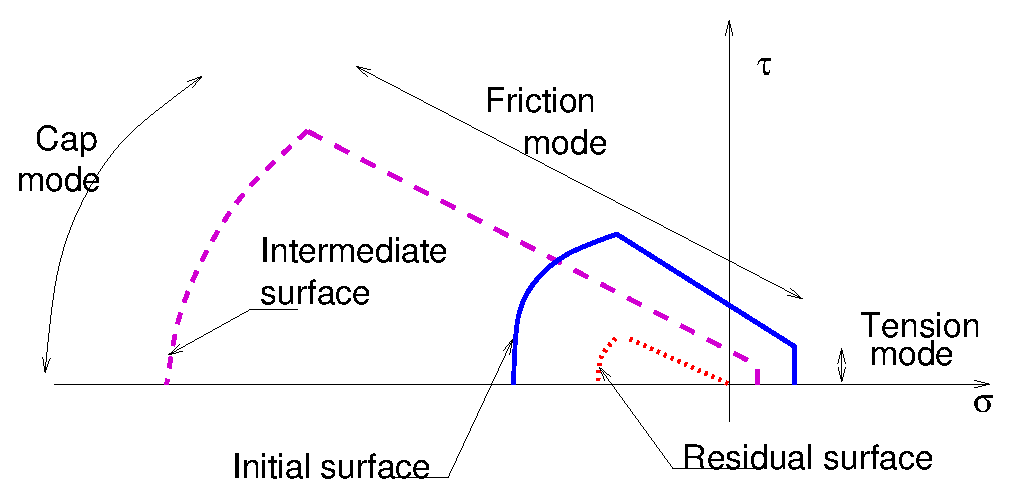
\includegraphics[width=0.7\textwidth]{constmodel.eps}}
\end{htmlonly}
%begin{latexonly}
 \centerline{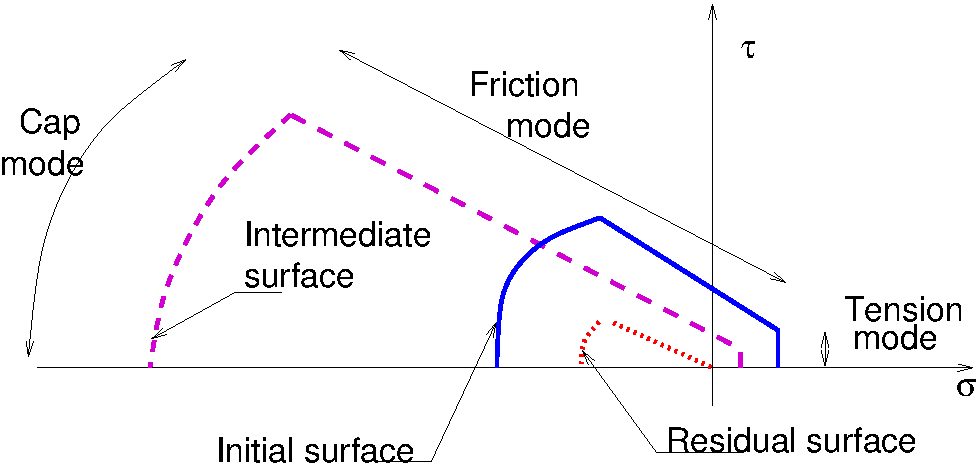
\includegraphics[width=0.7\textwidth]{constmodel}}
%end{latexonly}
  \caption{Composite yield surface model for masonry}
  \label{compyieldsurffig}
\end{figure}


The approach used in this work is based on idea of concentrating all the damage in the relatively weak joints and, if necessary, in potential tension cracks in the bricks. The joint interface constitutive model should include all important damage mechanisms. Here, the  concept of interface elements is used. An interface element allows to incorporate discontinuities in the displacement field and its behavior is described in terms of a relation between the tractions and relative displacement across the interface. In the present work, these quantities will be denoted as $\sig$, generalized stress, and $\e$, generalized strain. For 2D configuration, $\sig=\{\sigma, \tau\}^T$ and $\e=\{u_n, u_s\}^T$, where $\sigma$ and $\tau$ are the normal and shear components of the traction interface vector and  $n$ and $s$ subscripts distinguish between normal and shear components of displacement vector.
\begin{figure}[!htb]
\begin{htmlonly}
  \centerline{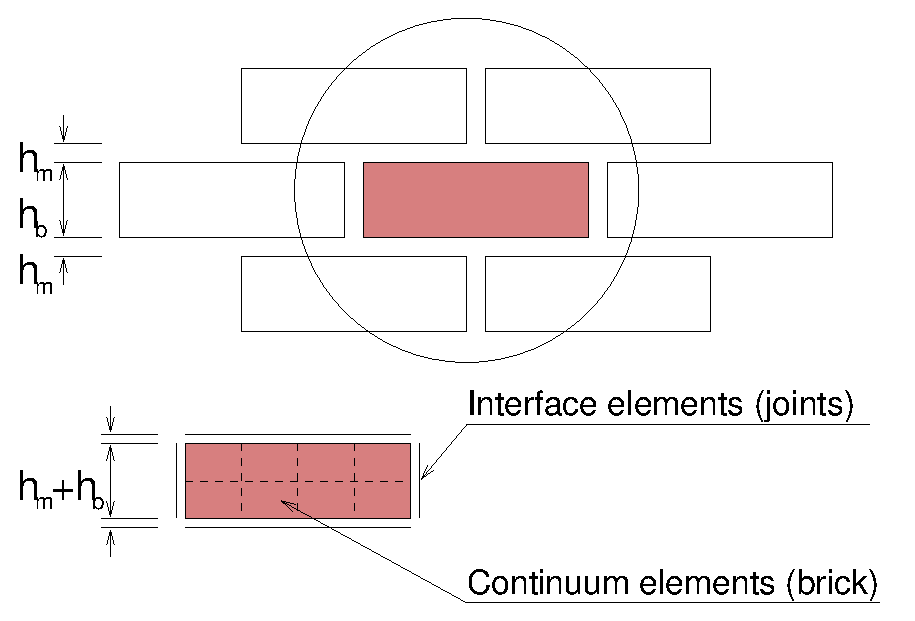
\includegraphics[width=0.7\textwidth]{mmodel.eps}}
\end{htmlonly}
%begin{latexonly}
 \centerline{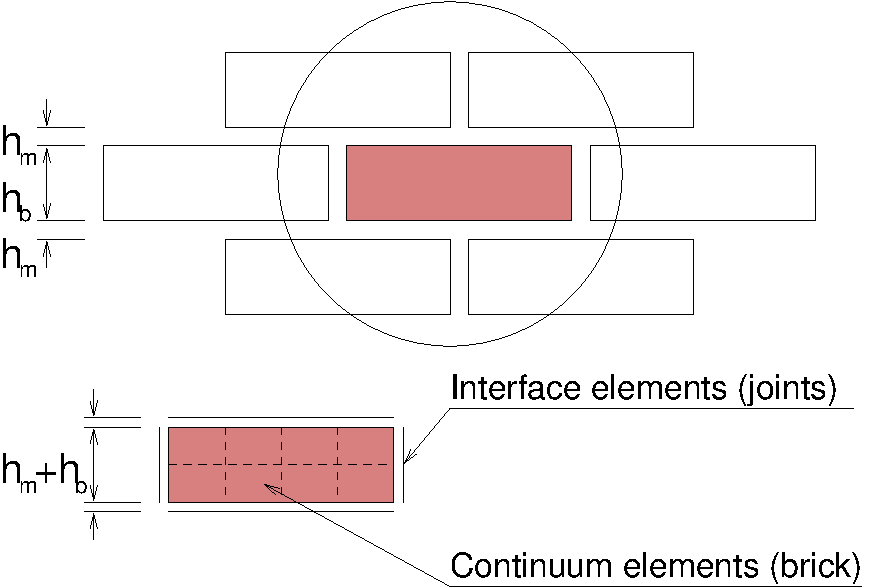
\includegraphics[width=0.7\textwidth]{mmodel}}
%end{latexonly}
  \caption{Modeling strategy for masonry}
\end{figure}
The elastic response is characterized in terms of elastic constitutive matrix $\mbf{D}$ as
\begin{equation}
  \sig=\mbf{D}\e
\end{equation}
For a 2D configuration $\mbf{D}=diag\{k_n,k_s\}$. The terms of the elastic stiffness matrix can be obtained from the properties of both masonry and joints as
\begin{equation}
  k_n=\del{E_bE_m}{t_m(E_b-E_m)};\;k_s=\del{G_bG_m}{t_m(G_b-G_m)}
\end{equation}
where $E_b$ and $E_m$ are Young's moduli, $G_b$ and $G_m$ shear moduli for brick and mortar, and $t_m$ is the thickness of joint. One should note, that there is no contact algorithm assumed between bricks, this means that the overlap of neighboring units will be visible. On the other hand, the interface model includes a compressive cap, where the compressive inelastic behavior of masonry is lumped.
\paragraph{Tension mode}
In the tension mode, the exponential softening law is assumed (see fig.(\ref{tensfig})). The yield function has the following form
\begin{equation}
  f_1(\sig,\kappa_1) = \sigma-f_t(\kappa_1)
\end{equation}
where the yield value $f_t$ is defined as
\begin{equation}
\label{ft}
  f_t=f_{t0}\exp\left(-\del{f_{t0}}{G^I_f}\kappa_1\right)
\end{equation}
\begin{figure}[!htb]
\begin{htmlonly}
  \centerline{\includegraphics[width=0.7\textwidth]{tension.eps}}
\end{htmlonly}
%begin{latexonly}
 \centerline{\includegraphics[width=0.7\textwidth]{tension}}
%end{latexonly}
  \caption{Tensile behavior of proposed model ($f_t=0.2$ MPa, $G_f^I=0.018$ N/mm)}
  \label{tensfig}
\end{figure}
The $f_{t0}$ represents tensile strength of joint or interface; and $G^I_f$ is mode-I fracture energy. For the tension mode, the associated flow hypothesis is assumed.


\paragraph{Shear mode}
For the shear mode a Coulomb friction envelope is used. The yield function has the form
\begin{equation}
  f_2(\sig,\kappa_2) = \vert\tau\vert+\sigma\tan\phi(\kappa_2)-c(\kappa_2)
\end{equation}
According to \cite{Rots} the variations of friction angle $\phi$ and cohesion $c$ are assumed as
\begin{eqnarray}
  \label{c}
  c&=&c_0\exp\left(-\del{c_0}{G^{II}_f}\kappa_2\right)\\
  \tan\phi&=&\tan\phi_0+(\tan\phi_r-\tan\phi_0)\left(\del{c_0-c}{c_0}\right)
\end{eqnarray}
where $c_0$ is initial cohesion of joint, $\phi_0$ initial friction angle, $\phi_r$ residual friction angle, and $G^{II}_f$ fracture energy in mode II failure. A non-associated plastic potential $g_2$ is considered as
\begin{equation}
  g_2=\vert\tau\vert+\sigma\tan\Phi-c
\end{equation}
\begin{figure}[!htb]
\begin{htmlonly}
  \centerline{\includegraphics[width=0.7\textwidth]{shearconf.eps}}
\end{htmlonly}
%begin{latexonly}
 \centerline{\includegraphics[width=0.7\textwidth]{shearconf}}
%end{latexonly}
  \caption{Shear behavior of proposed model for different confinement levels in MPa ($c_0=0.8\ \rm{MPa},\ \tan\phi_0=1.0,\ \tan\phi_r=0.75,{\rm and}\ G_f^{II}=0.05\ {N/mm}$)}
\end{figure}


\paragraph{Coupling of tension/shear modes}
The tension and Coulomb friction modes are coupled with isotropic softening. This means that the percentage of softening in the cohesion is assumed to be the same as on the tensile strength
\begin{equation}
  \dot\kappa_1=\lambda_1+\del{G^I_f}{G^{II}_f}\del{c_0}{f_{t0}}\lambda_2;\ \ \dot\kappa_2=\del{G^{II}_f}{G^I_f}\del{f_{t0}}{c_0}\lambda_1+\lambda_2
\end{equation}
This follows from (\ref{ft}) and (\ref{c}). However, in the corner region, when both yield surfaces are activated, such approach will lead to a non-acceptable penalty. For this reason a quadratic combination is assumed
\begin{equation}
  \dot\kappa_1=\sqrt{(\lambda_1)^2+\left(\del{G^I_f}{G^{II}_f}\del{c_0}{f_{t0}}\lambda_2\right)^2};\ \ \dot\kappa_2=\sqrt{\left(\del{G^{II}_f}{G^I_f}\del{f_{t0}}{c_0}\lambda_1\right)^2+(\lambda_2)^2}
\end{equation}

\paragraph{Cap mode}
For the cap mode, an ellipsoid interface model is used. The yield condition is assumed as
\begin{equation}
  f_3(\sig, \kappa_3) = C_{nn}\sigma^2+C_{ss}\tau^2 + C_n\sigma-\bar{\sigma}^2(\kappa_3)
\end{equation}
where $C_{nn},\ C_{ss}$, and $C_n$ are material model parameters and $\bar{\sigma}$ is yield value, originally assumed in the following form of hardening/softening law \cite{Rots}
\begin{eqnarray}
  \nonumber
  \bar{\sigma}_1(\kappa_3)&=&\bar{\sigma}_i+(\bar{\sigma}_p-\bar{\sigma}_i)\sqrt{\del{2\kappa_3}{\kappa_p}-\del{\kappa_3^2}{\kappa_p^2}};\;\;\kappa_3\in(0,\kappa_p)\\
  \label{hs3}
  \bar{\sigma}_2(\kappa_3)&=&\bar{\sigma}_p+(\bar{\sigma}_m-\bar{\sigma}_p)\left(\del{\kappa_3-\kappa_p}{\kappa_m-\kappa_p}\right)^2;\;\;\kappa_3\in(\kappa_p, \kappa_m)\\
  \nonumber
  \bar{\sigma}_3(\kappa_3)&=&\bar{\sigma}_r+(\bar{\sigma}_m-\bar{\sigma}_r)\exp\left(m\del{\kappa_3-\kappa_m}{\bar{\sigma}_m-\bar{\sigma}_r}\right);\;\;\kappa_3\in(\kappa_m, \infty)
\end{eqnarray}
with $m=2(\bar{\sigma}_m-\bar{\sigma}_p)/(\kappa_m-\kappa_p)$. The hardening/softening law (\ref{hs3}) is shown in fig.(\ref{hs3fig}). Note that the curved diagram is a $C^1$ continuous $\sigma-\kappa_3$ relation. The energy under the load-displacement diagram can be related to a ``compressive fracture energy''.
The original hardening law (\ref{hs3}.1) exhibits indefinite slope for $\kappa_3=0$, which can cause the problems with numerical implementation. This has been overcomed by replacing this hardening law with parabolic equation given by
\begin{equation}
  \bar{\sigma}_1(\kappa_3) = \bar{\sigma}_i-2*(\bar{\sigma}_i-\bar{\sigma}_p)*\del{\kappa_3}{\kappa_p}+(\bar{\sigma}_i-\bar{\sigma}_p)\del{\kappa_3}{\kappa_p}
\end{equation}
An associated flow and strain hardening hypothesis are being considered. This yields
\begin{equation}
  \dot\kappa_3=\lambda_3\sqrt{(2C_{nn}\sigma+C_n)*(2C_{nn}\sigma+C_n) + (2C_{ss}\tau)*(2C_{ss}\tau)}
\end{equation}
\begin{figure}[!htb]
\begin{htmlonly}
  \centerline{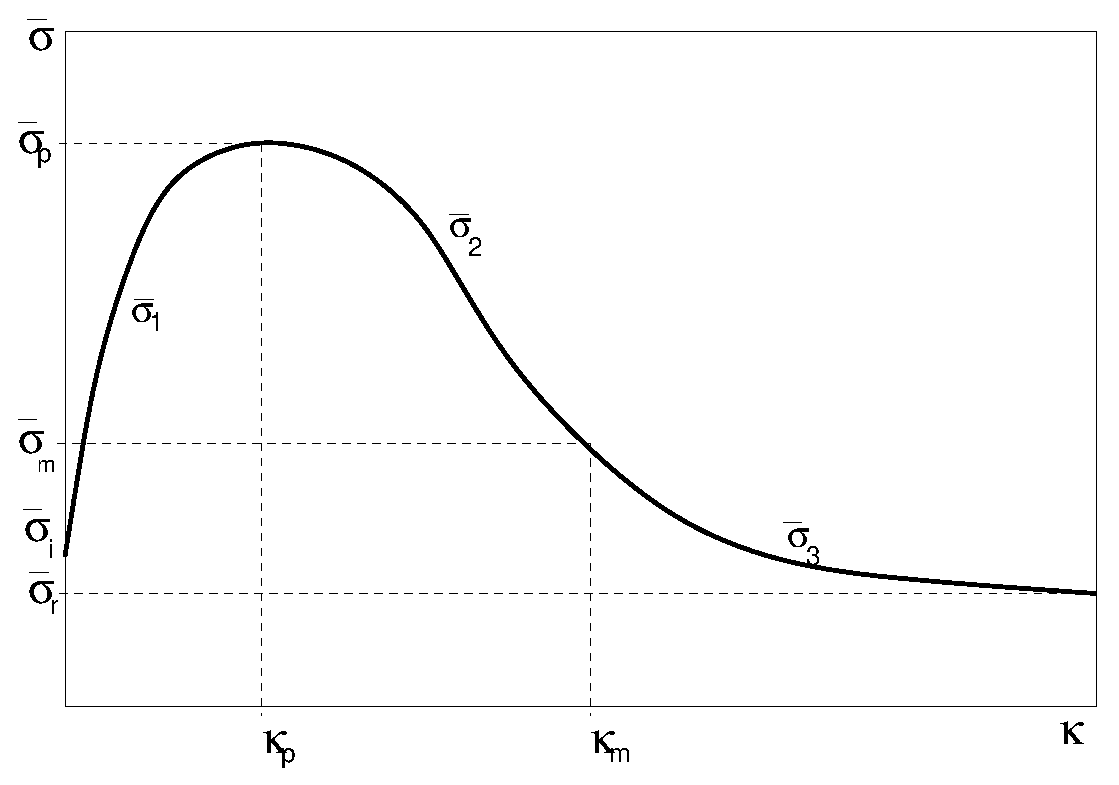
\includegraphics[width=0.7\textwidth]{capmode.eps}}
\end{htmlonly}
%begin{latexonly}
\centerline{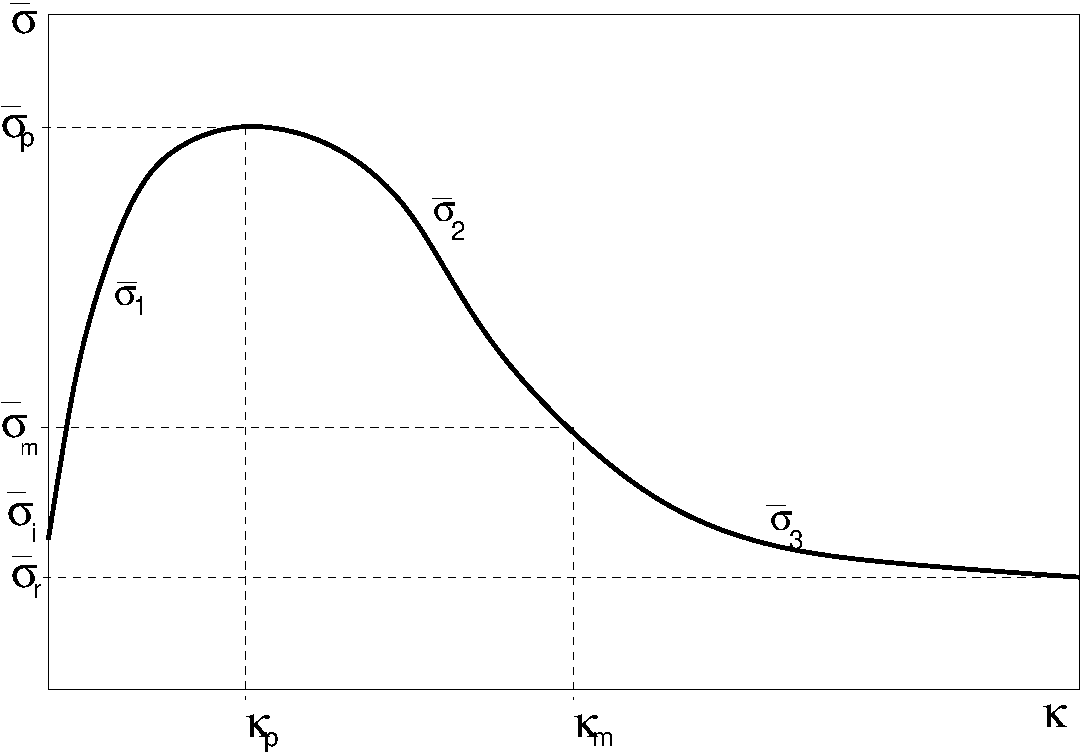
\includegraphics[width=0.7\textwidth]{capmode}}
%end{latexonly}
\caption{Hardening/softening law for cap mode}
\label{hs3fig}
\end{figure}

The model parameters are summarized in Tab.~\ref{compomasonry1_table}.
There is one algorithmic issue, that follows from the model
formulation. Since the cap mode hardening/softening is not coupled to
hardening/softening of shear and tension modes the it may happen that
when the cap and shear modes are activated, the return directions
become parallel for both surfaces. This should be avoided by adjusting
the input parameters accordingly (one can modify dilatancy angle, for example).

\begin{table}[!htb]
%\begin{center}
\begin{tabular}{|l|p{9cm}|}
\hline
Description & Composite plasticity model for masonry\\
\hline
Record Format & \descitem{Masonry02} \elemparam{num}{in} \elemparam{d}{rn} \elemparam{E}{rn}
\elemparam{n}{rn} \elemparam{ft0}{rn} \elemparam{gfi}{rn}
\elemparam{gfii}{rn}
\elemparam{kn}{rn} \elemparam{ks}{rn} \elemparam{c0}{rn}
\elemparam{tanfi0}{rn} \elemparam{tanfir}{rn} \elemparam{tanpsi}{rn}
\elemparam{si}{rn} \elemparam{sp}{rn} \elemparam{sm}{rn} \elemparam{sr}{rn}
\elemparam{kp}{rn} \elemparam{km}{rn} \elemparam{kr}{rn}
\elemparam{cnn}{rn} \elemparam{css}{rn} \elemparam{cn}{rn}\\
Parameters &- \param{num} material model number\\
&- \param{d} material density\\
&- \param{E} Young modulus\\
&- \param{n} Poisson ratio\\
&- \param{ft0} tensile strength\\
&- \param{gfi} fracture energy for mode I\\
&- \param{gfii} fracture energy for mode II\\
&- \param{kn} joint elastic property\\
&- \param{ks} joint elastic property\\
&- \param{c0} initial cohesion\\
&- \param{tanfi0} initial friction angle\\
&- \param{tanfir} residual friction angle\\
&- \param{tanpsi} dilatancy\\
&- \param{\{si, sp, sm, sr\}} cap parameters $\{\bar{\sigma}_i, \bar{\sigma}_p, \bar{\sigma}_m, \bar{\sigma}_r\}$\\
&- \param{\{kp, km,kr\}} cap parameters $\{\kappa_p, \kappa_m, \kappa_r\}$\\
&- \param{cnn},\param{css},\param{cn} cap mode parametrs\\
Supported modes& \_2dInterface\\
\hline
\end{tabular}
\caption{Composite model for masonry - summary.}
\label{compomasonry1_table}
%\end{center}
\end{table}



\subsubsection{Nonlinear elasto-plastic material model for concrete
plates and shells - Concrete2}
\label{Rer}
Nonlinear elasto-plastic material model with hardening.
Takes into account uniaxial stress + transverse shear in concrete
layers with transverse stirrups.
Can be used only for 2d plates and shells with layered cross section
and together with explicit integration method (stiffness matrix is not
provided).
The model description and parameters are summarized
in Tab.~\ref{Rer_table}.

\begin{table}[!htb]
%\begin{center}
\begin{tabular}{|l|p{9cm}|}
\hline
Description & Nonlinear elasto-plastic material model for concrete
plates and shells\\
\hline
Record Format & \descitem{Concrete2} \elemparam{num}{in}
\elemparam{d}{rn} \elemparam{E}{rn} \elemparam{n}{rn}
\elemparam{SCCC}{rn} \elemparam{SCCT}{rn} \elemparam{EPP}{rn} \elemparam{EPU}{rn}
\elemparam{EOPU}{rn} \elemparam{EOPP}{rn} \elemparam{SHEARTOL}{rn}
\elemparam{IS\_PLASTIC\_FLOW}{in} \elemparam{IFAD}{in} \elemparam{STIRR\_E}{rn} \elemparam{STIRR\_Ft}{rn}
\elemparam{STIRR\_A}{rn} \elemparam{STIRR\_TOL}{rn} \elemparam{STIRR\_EREF}{rn}
\elemparam{STIRR\_LAMBDA}{rn}\\

Parameters &- \param{num} material model number\\
&- \param{d} material density\\
&- \param{E} Young modulus\\
&- \param{n} Poisson ratio\\
&- \param{SCCC} pressure strength\\
&- \param{SCCT} tension strength\\
&- \param{EPP} threshold effective plastic strain for softening in
compression\\
&- \param{EPU} ultimate eff. plastic strain\\
&- \param{EOPP} threshold volumetric plastic strain for softening in
tension\\
&- \param{EOPU} ultimate volumetric plastic strain\\
&- \param{SHEARTOL} threshold value of the relative shear deformation
(psi**2/eef) at which shear is considered in layers.
For lower relative shear deformations the transverse shear remains elastic decoupled from bending. default value
SHEARTOL = 0.01\\
&- \param{IS\_PLASTIC\_FLOW} indicates that plastic flow (not
deformation theory) is used in pressure\\
&- \param{IFAD} State variables will not be updated, otherwise update state variables\\
&- \param{STIRR\_E} Young modulus of stirrups\\
&- \param{STIRR\_R} stirrups uniaxial strength = elastic limit\\
&- \param{STIRR\_A} stirrups area/unit length (beam) or /unit area (shell)\\
&- \param{STIRR\_TOL} stirrups tolerance of equilibrium in the z direction (=0 no iteration)\\
&- \param{STIRR\_EREF} stirrups reference strain rate for Peryzna's
material\\
&- \param{STIRR\_LAMBDA} coefficient for that material (stirrups)\\
&- \param{SHTIRR\_H} isotropic hardening factor for stirrups\\
Supported modes& 3dShellLayer, 2dPlateLayer\\
\hline
\end{tabular}
\caption{Nonlinear elasto-plastic material model for concrete - summary.}
\label{Rer_table}
%\end{center}
\end{table}





\subsection{Material models for tensile failure}
\subsubsection{Nonlinear elasto-plastic material model for concrete
plates and shells - Concrete2}
The description can be found is section~\ref{Rer}.



\subsubsection{Smeared rotating crack model - Concrete3}
\label{rcm}
Implementation of smeared rotating crack model.
Virgin material is modeled as isotropic linear elastic material
(described by Young modulus and Poisson
ratio). The onset of cracking begins, when principal stress reaches
tensile strength.
Further behavior is then determined by softening law,
governed by principle of preserving of fracture
energy $G_f$. For large elements, the tension strength can be
artificially reduced
to preserve fracture energy. Multiple cracks are allowed.
The elastic unloading and reloading is assumed.
In compression regime, this model correspond to isotropic linear elastic material.
The model description and parameters are summarized
in Tab.~\ref{rcm_table}.

\begin{table}[!htb]
%\begin{center}
\begin{tabular}{|l|p{9cm}|}
\hline
Description & Rotating crack model for concrete\\
\hline
Record Format & \descitem{Concrete3} \elemparam{d}{rn} \elemparam{E}{rn}
\elemparam{n}{rn} \elemparam{Gf}{rn} \elemparam{Ft}{rn} \elemparam{exp\_soft}{in} \elemparam{tAlpha}{rn} \\
Parameters &- \param{num} material model number\\
&- \param{d} material density\\
&- \param{E} Young modulus\\
&- \param{n} Poisson ratio\\
&- \param{Gf} fracture energy\\
&- \param{Ft} tension strength\\
&- \param{exp\_soft} determines the type of softening (0 =
exponential, 1 = linear)\\
&- \param{tAlpha} thermal dilatation coefficient\\
Supported modes& 3dMat, PlaneStress, PlaneStrain, 1dMat,
2dPlateLayer, 2dBeamLayer, 3dShellLayer\\
\hline
\end{tabular}
\caption{Rotating crack model for concrete - summary.}
\label{rcm_table}
%\end{center}
\end{table}



\subsubsection{Smeared rotating crack model with transition to scalar
damage - linear softening - RCSD}
\label{rcsd}
Implementation of smeared rotating crack model with transition to
scalar damage with linear softening law.
Improves the classical rotating model (see
section~\ref{rcm}) by introducing the transition to scalar damage
model in  later stages of tension softening.

Traditional smeared-crack models for concrete fracture are known to suffer by stress locking (meaning here spurious stress transfer across widely opening cracks),
mesh-induced directional bias, and possible instability at late stages of the loading process.
The combined model keeps the anisotropic character of the rotating
crack but it does not transfer spurious stresses across
widely open cracks.
The new model with transition to
scalar damage (RC-SD) keeps the anisotropic character of the RCM but
it does not transfer spurious stresses across widely open cracks.

Virgin material is modeled as isotropic linear elastic material
(described by Young modulus and Poisson
ratio). The onset of cracking begins, when principal stress reaches
tensile strength.
Further behavior is then determined by {\bf linear} softening law,
governed by principle of preserving of fracture
energy $G_f$. For large elements, the tension strength can be
artificially reduced
to preserve fracture energy.  The transition to scalar damage model
takes place, when the softening stress reaches the specified limit.
Multiple cracks are allowed.
The elastic unloading and reloading is assumed.
In compression regime, this model correspond to isotropic linear elastic material.
The model description and parameters are summarized
in Tab.~\ref{rcsd_table}.

\begin{table}[!htb]
%\begin{center}
\begin{tabular}{|l|p{9cm}|}
\hline
Description & Smeared rotating crack model with transition to scalar
damage - linear softening\\
\hline
Record Format & \descitem{RCSD} \elemparam{d}{rn} \elemparam{E}{rn}
\elemparam{n}{rn} \elemparam{Gf}{rn} \elemparam{Ft}{rn} \elemparam{sdtransitioncoeff}{rn} \elemparam{tAlpha}{rn} \\
Parameters &- \param{num} material model number\\
&- \param{d} material density\\
&- \param{E} Young modulus\\
&- \param{n} Poisson ratio\\
&- \param{Gf} fracture energy\\
&- \param{Ft} tension strength\\
&- \param{sdtransitioncoeff} determines the transition from RC to SD
model. Transition takes plase when ratio of current softening
stress to tension strength is less than  \param{sdtransitioncoeff} value\\
&- \param{tAlpha} thermal dilatation coefficient\\
Supported modes& 3dMat, PlaneStress, PlaneStrain, 1dMat,
2dPlateLayer, 2dBeamLayer, 3dShellLayer\\
\hline
\end{tabular}
\caption{RC-SD model for  concrete - summary.}
\label{rcsd_table}
%\end{center}
\end{table}



\subsubsection{Smeared rotating crack model with transition to scalar
damage - exponential softening - RCSDE}
\label{rcsde}
Implementation of smeared rotating crack model with transition to
scalar damage with exponential softening law.
The description and model summary (Tab.~\ref{rcsde_table}) are the
same as for the RC-SD model with linear softening law (see section~\ref{rcsd}).
\begin{table}[!htb]
%\begin{center}
\begin{tabular}{|l|p{9cm}|}
\hline
Description & Smeared rotating crack model with transition to scalar
damage - exponential softening\\
\hline
Record Format & \descitem{RCSDE} \elemparam{d}{rn} \elemparam{E}{rn}
\elemparam{n}{rn} \elemparam{Gf}{rn} \elemparam{Ft}{rn} \elemparam{sdtransitioncoeff}{rn} \elemparam{tAlpha}{rn} \\
\hline
\end{tabular}
\caption{RC-SD model for  concrete - summary.}
\label{rcsde_table}
%\end{center}
\end{table}



\subsubsection{Nonlocal smeared rotating crack model with transition to scalar damage - RCSDNL}
\label{rcsdnl}
Implementation of nonlocal version of smeared rotating crack model with transition to
scalar damage.
Improves the classical rotating model (see
section~\ref{rcm}) by introducing the transition to scalar damage
model in  later stages of tension softening.
The improved RC-SD (see section~\ref{rcsd}) is further extended to a
nonlocal formulation, which not only acts as a powerful localization
limiter but also alleviates mesh-induced directional bias. A special
type of material instability arising due to negative shear stiffness
terms in the rotating crack model is resolved by switching to SD mode. A bell shaped nonlocal
averaging function is used.

Virgin material is modeled as isotropic linear elastic material
(described by Young modulus and Poisson
ratio). The onset of cracking begins, when principal stress reaches
tensile strength.
Further behavior is then determined by {\bf exponential} softening law.

The transition to scalar damage model
takes place, when the softening stress reaches the specified limit or
when the loss of material stability due to negative shear stiffness
terms that may arise in the standard RCM formulation, which takes
place when the ratio of minimal shear coefficient in stiffness to
bulk material shear modulus reaches the limit.

Multiple cracks are allowed.
The elastic unloading and reloading is assumed.
In compression regime, this model correspond to isotropic linear elastic material.
The model description and parameters are summarized
in Tab.~\ref{rcsdnl_table}.

\begin{table}[!htb]
%\begin{center}
\begin{tabular}{|l|p{9cm}|}
\hline
Description & Nonlocal smeared rotating crack model with transition to scalar damage for concrete\\
\hline
Record Format & \descitem{RCSDNL} \elemparam{d}{rn} \elemparam{E}{rn}
\elemparam{n}{rn}  \elemparam{Ft}{rn}
\elemparam{sdtransitioncoeff}{rn} \elemparam{sdtransitioncoeff2}{rn}
\elemparam{r}{rn} \elemparam{tAlpha}{rn} \\
Parameters &- \param{num} material model number\\
&- \param{d} material density\\
&- \param{E} Young modulus\\
&- \param{n} Poisson ratio\\
&- \param{ef} deformation corresponding to fully open crack\\
&- \param{Ft} tension strength\\
&- \param{sdtransitioncoeff} determines the transition from RC to SD
model. Transition takes place when ratio of current softening
stress to tension strength is less than  \param{sdtransitioncoeff} value\\
&- \param{sdtransitioncoeff2} determines the transition from RC to SD
model. Transition takes place when ratio of current minimal shear
stiffness term to virgin shear modulus is less than  \param{sdtransitioncoeff2} value\\
&- \param{r} parameter specifying the width of nonlocal averaging zone\\
&- \param{tAlpha} thermal dilatation coefficient\\
&- \param{regionMap} map indicating the regions (currently region is
characterized by cross section number) to skip for nonlocal
avaraging. The elements and corresponding IP are not taken into
account in nonlocal averaging process if corresponding regionMap
value is nonzero.\\
Supported modes& 3dMat, PlaneStress, PlaneStrain, 1dMat,
2dPlateLayer, 2dBeamLayer, 3dShellLayer\\
\hline
\end{tabular}
\caption{RC-SD-NL model for  concrete - summary.}
\label{rcsdnl_table}
%\end{center}
\end{table}



\subsubsection{Isotropic damage model for tensile failure - Idm1}
\label{sec:idmtf}
This isotropic damage model assumes that the stiffness degradation is
isotropic, i.e., stiffness moduli corresponding to different
directions decrease proportionally and independently of the loading 
direction. The damaged stiffness tensor is expressed as
$\mbf{D}=(1-\omega)\mbf{D}_e$ where $\omega$ is a scalar damage variable
and $\mbf{D}_e$ is the elastic stiffness tensor.
The damage evolution law is postulated in an explicit form, relating
the damage variable $\omega$ to the largest previously reached 
equivalent strain level, $\kappa$.

The equivalent strain, $\tilde\varepsilon$, is a scalar measure derived from the
strain tensor. The choice of the specific expression
for the equivalent strain affects the shape of the elastic domain
in the strain space and plays a similar role to the choice of a yield
condition in plasticity.
The following definitions of equivalent strain are currently supported:
\begin{itemize}
\item
{\bf Mazars} (1984) definition based on norm of positive part of strain:
\begin{equation}
\label{mazars}
\tilde\varepsilon=\sqrt{\displaystyle{\sum_{I=1}^{3}}\langle\varepsilon_I\rangle^2}
\end{equation}
where $\langle\varepsilon_I\rangle$ are positive parts of 
principal values of the strain tensor $\mbf{\varepsilon}$.
\item
Definitions derived from the {\bf Rankine} criterion of maximum principal stress:
\begin{eqnarray}
\label{rankinesmooth}
\tilde\varepsilon&=&
{\del{1}{E}}\sqrt{\displaystyle{\sum_{I=1}^{3}}\langle\bar{\sigma}_I\rangle^2}
\\
\label{rankinestandard}
\tilde\varepsilon&=&
{\del{1}{E}}\max_{I=1}^{3}\bar{\sigma}_I
\end{eqnarray}
where
$\bar{\sigma}_I$, $I=1,2,3$, are the principal 
values of the
effective stress tensor $\bar{\mbf{\sigma}} = \mbf{D}_e:\mbf{\varepsilon}$
and $\langle\bar{\sigma}_I\rangle$ are their positive parts.
\item
{\bf Energy} norm scaled by Young's modulus to obtain
a strain-like quantity:
\begin{equation}
\label{energynorm}
\tilde\varepsilon=\del{1}{E}\sqrt{{\mbf{\varepsilon}:\mbf{D}_e:\mbf{\varepsilon}}}
\end{equation}
\item
{\bf Modified Mises} definition, proposed by de Vree \cite{Vree:95}:
\begin{equation}
\label{modifiedmises}
\tilde\varepsilon=\frac{(k-1)I_{1\varepsilon}}{2k(1-2\nu)} + \frac{1}{2k}\sqrt{\frac{(k-1)^2}{(1-2\nu)^2}I_{1\varepsilon}^2+\frac{12 k J_{2\varepsilon}}{(1+\nu)^2}} 
\end{equation}
where $$
I_{1\varepsilon} = \sum_{I=1}^3\varepsilon_I
$$
is the first strain invariant (trace of the strain tensor),
$$
J_{2\varepsilon} = \frac{1}{2}\sum_{I=1}^3 \varepsilon_I^2-\frac{1}{6}I_{1\varepsilon}^2
$$  
is the second deviatoric strain invariant,
and $k$ is a model parameter that corresponds to the ratio between the uniaxial
compressive strength $f_c$ and uniaxial tensile strength $f_t$.
\end{itemize}
Note that all these definitions are based on the three-dimensional
description of strain (and stress). If they are used in a reduced
problem, the strain components that are not explicitly provided by
the finite element approximation are computed from the underlying 
assumptions and used in the evaluation of equivalent strain.
For instance, in a plane-stress analysis, the out-of-plane component
of normal strain is calculated from the assumption of zero
out-of-plane normal stress (using standard Hooke's law).

Since the growth of damage usually leads to softening and may induce
localization of the dissipative process, attention should be paid
to proper regularization. The most efficient approach is based on
a nonlocal formulation; see Section~\ref{sec:nidm}. 
If the model is kept local, the damage law
should be adjusted according to the element size, in the spirit
of the crack-band approach. When done properly, this ensures
a correct dissipation of energy in a localized band of cracking
elements, corresponding to the fracture energy of the material.
For various numerical studies, it may be useful to specify the
parameters of the damage law directly, independently of the element size.
One should be aware that in this case the model would exhibit
pathological sensitivity to the size of finite elements if the mesh
is changed. 

The following damage laws are currently implemented:
\begin{itemize}
\item
{\bf Cohesive crack with exponential softening} postulates a relation
between the normal stress $\sigma$ transmitted by the crack and the
crack opening $w$ in the form
$$
\sigma = f_t\exp\left(-\frac{w}{w_f}\right)
$$
Here, $f_t$ is the tensile strength and $w_f$ is a parameter with the dimension
of length (crack opening), which controls the ductility of the material.
In fact, $w_f=G_f/f_t$ where $G_f$ is the mode-I fracture energy.
In the context of the crack-band approach, the crack opening $w$ corresponds
to the inelastic (cracking) strain $\varepsilon_c$ 
multiplied by the effective thickness $h$ of the 
crack band. The effective thickness $h$ is estimated by projecting the finite
element onto the direction of the maximum principal strain (and stress)
at the onset of damage. The inelastic strain $\varepsilon_c$
is the difference between
the total strain $\varepsilon$ and the elastic strain $\sigma/E$.
For the damage model we obtain
$$
\varepsilon_c = \varepsilon - \frac{\sigma}{E} =
\varepsilon - (1-\omega)\varepsilon = \omega\varepsilon
$$
and thus $w=h\varepsilon_c=h\omega\varepsilon$. Substituting this into
the cohesive law and combining with the stress-strain law for the damage
model, we get a nonlinear equation
$$
(1-\omega)E\varepsilon = f_t\exp\left(-\frac{h\omega\varepsilon}{w_f}\right)
$$
For a given strain $\varepsilon$, the corresponding damage variable $\omega$
can be solved from this equation by Newton iterations. 
It can be shown that the solution exists and is unique for every
$\varepsilon\ge\varepsilon_0$ provided that the element size $h$ does not
exceed the limit size $h_{max}=w_f/\varepsilon_0$. For larger elements,
a local snapback in the stress-strain diagram would occur, which is not
admissible. In terms of the material properties, $h_{max}$ can be expressed
as $EG_f/f_t^2$, which is related to Irwin's characteristic length.

The derivation
has been performed for monotonic loading and uniaxial tension. Under general
conditions, $\varepsilon$ is replaced by the internal variable $\kappa$,
which represents the maximum previously reached level of equivalent strain.

In the list of input variables, the tensile strength $f_t$ is not specified
directly but through the corresponding strain at peak stress, 
$\varepsilon_0=f_t/E$, denoted by keyword {\it e0}. Another input parameter
is the characteristic crack opening $w_f$, denoted by keyword {\it wf}.
\item
{\bf Cohesive crack with linear softening} is based on the same correspondence
between crack opening and inelastic strain, but the cohesive law is assumed
to have a simpler linear form
$$
\sigma = f_t\left(1-\frac{w}{w_f}\right)
$$
The relation between damage and strain can then be derived from the cohesive law and 
substituing $w=h \omega \varepsilon$
$$
\sigma = (1-\omega)E\varepsilon =  f_t\left(1-\frac{h \omega \varepsilon}{w_f}\right),
$$
which leads to explicit evaluation of the damage variable
$$
\omega=\frac{1-\displaystyle\frac{\varepsilon_0}{\varepsilon}}{1-\displaystyle\frac{h\varepsilon_0}{w_f}}
$$
and no iteration is needed. Parameter $w_f$,
denoted again by keyword {\it wf}, has now the meaning of crack opening
at complete failure (zero cohesive stress) and is related to fracture energy by
a modified formula $w_f=2G_f/f_t$.
The expression for maximum element size, $h_{max}=w_f/\varepsilon_0$, remains
the same as for cohesive law with exponential softening, but in terms
of the material properties it is now translated as $h_{max}=2EG_f/f_t^2$.
\item
{\bf Cohesive crack with bilinear softening} is implemented in an
approximate fashion and gives for different mesh sizes the same
total dissipation but different shapes of the softening diagram.
Instead of properly transforming the crack opening into inelastic strain,
the current implementation deals with a stress-strain diagram adjusted
such that the areas marked in the right part of Fig.~\ref{idm_softening}
are equal to the fracture energies $G_f$ and $G_{ft}$ divided by the
element size. The third parameter defining the law is the strain
$\eps_k$ at which the softening diagram changes slope. Since this
strain is considered as fixed, the corresponding stress $\sigma_k$
depends on the element size and for small elements gets close to the
tensile strength (the diagram then gets close to linear softening
with fracture energy  $G_{ft}$). 
\item
{\bf Linear softening stress-strain law} works directly with strain
and does not make any adjustment for the element size. The specified
parameters $\varepsilon_0$ and $\varepsilon_f$, denoted by keywords {\it e0}
and {\it ef}, have the meaning of (equivalent) strain at peak stress and at
complete failure. The linear relation between stress and strain on the
softening branch is obtained with the damage law
$$
\omega =\frac{\varepsilon_f}{\varepsilon_f-\varepsilon_0}\left(1-\frac{\varepsilon_0}{\varepsilon}\right)
$$
Again, to cover general conditions, $\varepsilon$ is replaced by $\kappa$.
\item
{\bf Exponential softening stress-strain law} also uses two parameters
 $\varepsilon_0$ and $\varepsilon_f$, denoted by keywords {\it e0}
and {\it ef}, but leads to a modified dependence of damage on strain:
$$
\omega =1-\frac{\varepsilon_0}{\varepsilon}\exp\left(-\frac{\varepsilon-\varepsilon_0}{\varepsilon_f-\varepsilon_0}\right)
$$
\item
{\bf Mazars stress-strain law} uses three parameters, $\varepsilon_0$,
$A_t$ and $B_t$, denoted by keywords {\it e0}, {\it At} and {\it Bt}, and the
dependence of damage on strain is given by
$$
\omega =1-\frac{(1-A_t)\varepsilon_0}{\varepsilon}-A_t\exp\left(B_t(\varepsilon-\varepsilon_0)\right)
$$
\item
{\bf Smooth exponential stress-strain law} uses two parameters, $\varepsilon_0$
and $M_d$, denoted by keywords {\it e0} and {\it md}, and the
dependence of damage on strain is given by
$$
\omega = 1-\exp\left(-\left(\frac{\varepsilon}{\varepsilon_0}\right)^{M_d}\right)
$$
This leads to a stress-strain curve that immediately deviates from linearity
(has no elastic part) and smoothly changes from hardening to softening,
with tensile strength
$$
f_t = E\varepsilon_0\left({\rm e}M_d\right)^{-1/M_d}
$$
\item
{\bf Extended smooth stress-strain law} is a special formulation used
by Grassl and Jir\'{a}sek (2010). The damage law has a rather complicated form:
\begin{equation} \label{eq:damageEvol}
\omega = \left \{ \begin{array}{ll} 
1-\exp\left(-\displaystyle\frac{1}{m}\left(\dfrac{\eps}{\varepsilon_{\rm p}}\right)^m\right) & \mbox{if $\eps \leq \varepsilon_1$}\\[2mm]
1- \dfrac{\varepsilon_3}{\eps} \exp \left(- \dfrac{\eps- \varepsilon_1}{\varepsilon_{\rm f} \left[1+ \left(\frac{\eps-\varepsilon_1}{\varepsilon_2}\right)^n\right]}\right) & \mbox{if $\eps > \varepsilon_1$} \end{array} \right.
\end{equation}
The primary model parameters are the uniaxial tensile strength $f_{\rm t}$,
the strain at peak stress (under uniaxial tension) $\varepsilon_{\rm p}$, and additional parameters
$\varepsilon_1$, $\varepsilon_2$ and $n$, which control the post-peak part of the stress-strain law. In the input record, they are denoted by keywords
\param{ft, ep, e1, e2, nd}.
Other parameters that appear in (\ref{eq:damageEvol}) can be derived from the condition of zero
slope of the stress-strain curve at $\kappa=\varepsilon_{\rm p}$ and from the conditions of stress and
stiffness continuity at $\kappa=\varepsilon_1$:
\begin{eqnarray}\label{eqparams1}
m&=&\frac{1}{\ln(E\varepsilon_{\rm p}/f_{\rm t})}\\
\label{eqparams2}
\varepsilon_{\rm f}&=&\frac{\varepsilon_1}{\left(\varepsilon_1/\varepsilon_{\rm p}\right)^m -1}\\
\varepsilon_3&=&\varepsilon_1\exp\left(-\frac{1}{m}\left(\frac{\varepsilon_1}{\varepsilon_p}\right)^m\right)
\label{eqparams3}
\end{eqnarray}
\end{itemize} 

Note that parameter {\it damlaw} determines which type of damage law
should be used, but the adjustment for element size is done only if
parameter {\it wf} is specified for {\it damlaw}=0 or {\it damlaw}=1. 
For other values of {\it damlaw}, or if parameter {\it ef} 
is specified instead of {\it wf}, the stress-strain curve does not depend
on element size and the model would exhibit pathological sensitivity
to the mesh size. These cases are intended to be used in combination
with a nonlocal formulation. An alternative formulation uses fracture energy
to determine fracturing strain.

The model parameters are summarized in Tab.~\ref{id_table}. Figure~\ref{idm_softening} shows
three modes of a softening law with corresponding variables.

\begin{figure}[!htb]
\begin{htmlonly}
  \centerline{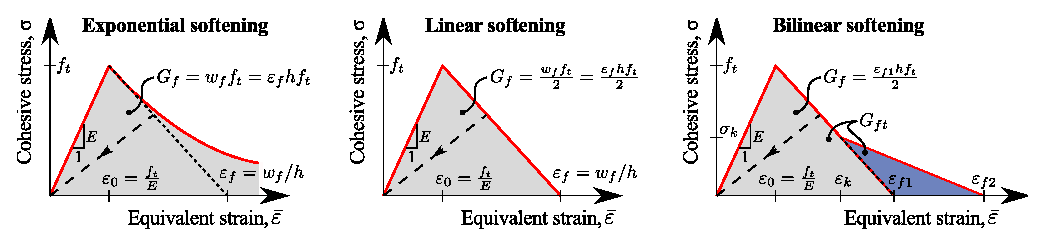
\includegraphics[width=0.99\textwidth]{Damage_material_diag.eps}}
\end{htmlonly}
%begin{latexonly}
 \centerline{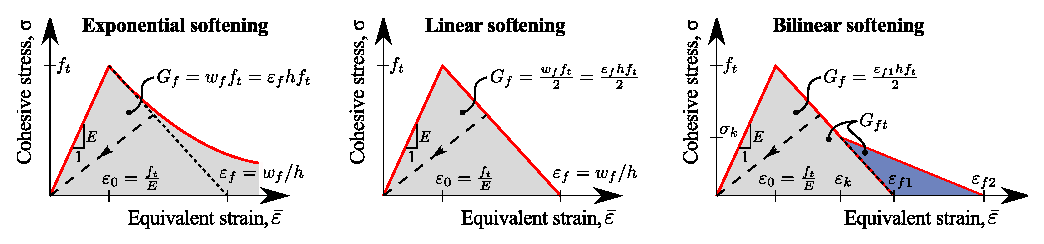
\includegraphics[width=0.99\textwidth]{Damage_material_diag}}
%end{latexonly}
  \caption{Implemented stress-strain diagrams for isotropic damage material. Fracturing strain $\varepsilon_f$ and crack opening at zero stress $w_f$ are interrelated through effective thickness $h$ of the crack band. Note that the
figure is somewhat misleading because the grey area is not $G_f$ but $G_f/h$ 
and also because for exponential softening the approach based on an exponential cohesive law is not exactly equivalent to the approach based on an exponential softening branch of the stress-strain diagram; see the detailed discussion of the damage laws.}
  \label{idm_softening}
\end{figure}


\begin{table}[!htb]
%\begin{center}
  \small
\begin{tabular}{|l|p{9cm}|}
\hline
Description & Isotropic damage model for concrete in tension\\
\hline
Record Format & \descitem{Idm1} 
\elemparam{}{in} 
\elemparam{d}{rn} 
\elemparam{E}{rn}
\elemparam{n}{rn} 
[\elemparam{tAlpha}{rn}] 
[\elemparam{equivstraintype}{in}] 
[\elemparam{k}{rn}]
[\elemparam{damlaw}{in}] 
\elemparam{e0}{rn}
[\elemparam{wf}{rn}] 
[\elemparam{ef}{rn}]
[\elemparam{ek}{rn}]
[\elemparam{gf}{rn}]
[\elemparam{gft}{rn}]
[\elemparam{At}{rn}] 
[\elemparam{Bt}{rn}] 
[\elemparam{md}{rn}] 
[\elemparam{ft}{rn}] 
[\elemparam{ep}{rn}] 
[\elemparam{e1}{rn}] 
[\elemparam{e2}{rn}] 
[\elemparam{nd}{rn}] 
[\elemparam{maxOmega}{rn}]
[\elemparam{checkSnapBack}{rn}]\\
Parameters &- \param{} material number\\
&- \param{d} material density\\
&- \param{E} Young's modulus\\
&- \param{n} Poisson's ratio\\
&- \param{tAlpha} thermal expansion coefficient\\
&- \param{equivstraintype} allows to choose from different definitions
of equivalent strain:
\begin{itemize}\setlength{\itemsep}{-3pt}
\item[0 -] default = Mazars, eq.~(\ref{mazars})
\item[1 -] smooth Rankine, eq.~ (\ref{rankinesmooth})
\item[2 -] scaled energy norm,  eq.~(\ref{energynorm})
\item[3 -] modified Mises, eq.~(\ref{modifiedmises})
\item[4 -] standard Rankine, eq.~(\ref{rankinestandard})
\end{itemize}\\
&- \param{k} ratio between uniaxial compressive and tensile strength, needed only if equivstraintype=3, default value 1\\
&- \param{damlaw} allows to choose from different damage laws:
\begin{itemize}\setlength{\itemsep}{-3pt}
\item[0 -] exponential softening (default) with parameters e0 and wf $\vert$ ef $\vert$ gf
\item[1 -] linear softening with parameters e0 and wf $\vert$ ef $\vert$ gf
\item[2 -] bilinear softening with gf, gft, ek
\item[3 -] Hordijk softening (not implemented yet)
\item[4 -] Mazars damage law with parameters At and Bt
\item[5 -] smooth stress-strain curve with parameters e0 and md
\item[6 -] disable damage (dummy linear elastic material)
\item[7 -] extended smooth damage law (\ref{eq:damageEvol}) with parameters ft, ep, e1, e2, nd
\end{itemize}\\
&- \param{e0} strain at peak stress (for damage laws 0,1,2,3), limit elastic strain (for damage law 4), characteristic strain (for damage law 5)\\
&- \param{wf} parameter controling ductility, has the meaning of crack opening (for damage laws 0 and 1)\\
&- \param{ef} parameter controling ductility, has the meaning of strain (for damage laws 0 and 1)\\
&- \param{ek} strain at knee point in bilinear softening type (for damage law 2)\\
&- \param{gf} fracture energy (for damage laws 0--2)\\
&- \param{gft} total fracture energy (for damage law 2)\\
&- \param{At} parameter of Mazars damage law, used only by law 4\\
&- \param{Bt} parameter of Mazars damage law, used only by law 4\\
&- \param{md} exponent used only by damage law 5, default value 1\\
&- \param{ft} tensile strength, used only by damage law 7\\
&- \param{ep} strain at peak stress, used only by damage law 7\\
&- \param{e1} parameter used only by damage law 7\\
&- \param{e2} parameter used only by damage law 7\\
&- \param{nd} exponent used only by damage law 7\\
&- \param{maxOmega} maximum damage, used for convergence improvement
(its value is between 0 and 0.999999 (default), and it affects only the secant stiffness
but not the stress)\\
&- \param{checkSnapBack} parameter for snap back checking, 0 no check, 1 check (default)\\
Supported modes& 3dMat, PlaneStress, PlaneStrain, 1dMat\\
Features & Adaptivity support\\
\hline
\end{tabular}
\caption{Isotropic damage model for tensile failure -- summary.}
\label{id_table}
%\end{center}
\end{table}

\subsubsection{Nonlocal isotropic damage model for tensile failure - Idmnl1}
\label{sec:nidm}
Nonlocal version of isotropic damage model from Section~\ref{sec:idmtf}.
The nonlocal averaging acts as a powerful localization
limiter. 
In the standard version of the model, 
damage is driven by the nonlocal equivalent strain $\bar{\varepsilon}$, 
defined as a weighted average of the local equivalent strain:
$$
\bar{\varepsilon}(\mbf{x}) = \int_V\alpha(\mbf{x},\mbf{\xi})\tilde\varepsilon(\mbf{\xi})\;{\rm d}\mbf{\xi}
$$
In the ``undernonlocal'' formulation, the damage-driving variable is a 
combination of local and nonlocal equivalent strain, 
$m\bar{\varepsilon}+(1-m)\tilde\varepsilon$, where $m$ is a parameter between
0 and 1. (If $m>1$, the formulation is called ``overnonlocal''; this case
is useful for nonlocal plasticity but not for nonlocal damage.) 

Instead
of averaging the equivalent strain, one can average the compliance variable
$\gamma$, directly related to damage according to the formula 
$\gamma=\omega/(1-\omega)$.

The weight function $\alpha$ contains a certain parameter with the dimension
of length, which is in general called the characteristic length. Its specific
meaning depends on the type of weight function. The following functions are
currently supported:
\begin{itemize}
\item
Truncated quartic spline, also called the bell-shaped function,
$$
\alpha_0(s) = \left\langle 1-\frac{s^2}{R^2}\right\rangle^2
$$
where $R$ is the interaction radius (characteristic length) and 
$s$ is the distance between the interacting points. This function 
is exactly zero for $s\ge R$, i.e., it has a bounded support.
\item
Gaussian function
$$
\alpha_0(s) = \exp\left(-\frac{s^2}{R^2}\right)
$$
which is theoretically nonzero for an arbitrary large $s$ and thus
has an unbounded support. However, in the numerical implementation
the value of $\alpha_0$ is considered as zero for $s>2.5R$.
\item
Exponential function
$$
\alpha_0(s) = \exp\left(-\frac{s}{R}\right)
$$
which also has an unbounded support, but is considered as zero for $s>6R$.
This function is sometimes called the Green function, because in 1D it
corresponds to the Green function of the Helmholtz-like equation used
by implicit gradient approaches.
\item
Piecewise constant function
$$
\alpha_0(s) =\left\{\begin{array}{cc} 1 & \mbox{ if } s\le R \\ 0 & \mbox{ if } s> R \end{array}\right.
$$
which corresponds to uniform averaging over a segment, disc or ball
of radius $R$. 
\item
Function that is constant over the finite element in which point $\mbf{x}$
is located, and is zero everywhere else. Of course, this is not a physically
objective definition of nonlocal averaging, since it depends on the
discretization. However, this kind of averaging was proposed in a boundary
layer by Prof.\ Ba\v{z}ant and was implemented into OOFEM for testing purposes.
\end{itemize}  
 
The above functions depend only on the distance $s$ between the interacting
points and are not normalized. If the normalizing
condition
$$
\int_{V_\infty} \alpha(\mbf{x},\mbf{\xi})\;{\rm d}\mbf{\xi} = 1
$$
is imposed in an infinite body $V_{\infty}$, it is sufficient to scale
$\alpha_0$ by a constant and set
$$
\alpha(\mbf{x},\mbf{\xi})=\frac{\alpha_0(\Vert\mbf{x}-\mbf{\xi}\Vert)}{V_{r\infty}}
$$
where
$$
V_{r\infty} = \int_{V_\infty} \alpha_0(\Vert\mbf{\xi}\Vert)\;{\rm d}\mbf{\xi} 
$$
Constant $V_{r\infty}$ can be computed analytically depending on the specific
type of weight function and the number of spatial dimensions in which the
analysis is performed. Since the factor $1/V_{r\infty}$ can be incorporated directly
in the definition of $\alpha_0$, this case is referred to as ``no scaling''.

If the body of interest is finite (or even semi-infinite), the averaging
integral can be performed only over
the domain filled by the body, and the volume contributing to the nonlocal
average at a point $\mbf{x}$ near the boundary is reduced as compared to 
points  $\mbf{x}$ far from the boundary or in an infinite body. To make sure
that the normalizing condition
$$
\int_{V} \alpha(\mbf{x},\mbf{\xi})\;{\rm d}\mbf{\xi} = 1
$$
holds for the specific domain $V$, different approaches can be used.
The standard approach defines the nonlocal weight function as  
$$
\alpha(\mbf{x},\mbf{\xi})=\frac{\alpha_0(\Vert\mbf{x}-\mbf{\xi}\Vert)}{V_r(\mbf{x})}
$$
where
$$
V_r(\mbf{x}) = \int_{V} \alpha_0(\Vert\mbf{x}-\mbf{\xi}\Vert)\;{\rm d}\mbf{\xi} 
$$
According to the approach suggested by Borino, the weight function is defined as
$$
\alpha(\mbf{x},\mbf{\xi})=\frac{\alpha_0(\Vert\mbf{x}-\mbf{\xi}\Vert)}{V_{r\infty}} + \left(1-\frac{V_r(\mbf{x})}{V_{r\infty}}\right)\delta(\mbf{x}-\mbf{\xi})
$$
where $\delta$ is the Dirac distribution. One can also say that the
nonlocal variable is evaluated as
$$
\bar{\varepsilon}(\mbf{x}) = \frac{1}{V_{r\infty}}\int_V\alpha_0(\Vert\mbf{x}-\mbf{\xi}\Vert)\tilde\epsilon(\mbf{\xi})\;{\rm d}\mbf{\xi}+\left(1-\frac{V_r(\mbf{x})}{V_{r\infty}}\right)\tilde\varepsilon(\mbf{x})
$$
The term on the right-hand side after the integral is a multiple of the local
variable, and so it can be referred to as the local complement.  

The model parameters are summarized
in Tabs.~\ref{idnl_table} and \ref{idnl_table_cont}.


\begin{table}[!htb]
\begin{tabular}{|l|p{9cm}|}
\hline
Description & Nonlocal isotropic damage model for concrete in tension\\
\hline
Record Format & \descitem{Idmnl1} 
\elemparam{}{in} 
\elemparam{d}{rn} 
\elemparam{E}{rn}
\elemparam{n}{rn}  
[\elemparam{tAlpha}{rn}]
[\elemparam{equivstraintype}{in}] 
[\elemparam{k}{rn}] 
[\elemparam{damlaw}{in}] 
\elemparam{e0}{rn}
[\elemparam{ef}{rn}] 
[\elemparam{At}{rn}] 
[\elemparam{Bt}{rn}] 
[\elemparam{md}{rn}] 
\elemparam{r}{rn}
[\elemparam{regionMap}{ia}]
[\elemparam{wft}{in}]
[\elemparam{averagingType}{in}]
[\elemparam{m}{rn}]
[\elemparam{scaling}{in}]
[\elemparam{averagedVar}{in}]
[\elemparam{maxOmega}{rn}]\\
Parameters &- \param{} material number\\
&- \param{d} material density\\
&- \param{E} Young's modulus\\
&- \param{n} Poisson's ratio\\
&- \param{tAlpha} thermal expansion coefficient\\
&- \param{equivstraintype} allows to choose from different definitions
of equivalent strain, same as for the local model; see Tab.~\ref{id_table}\\
&- \param{k} ratio between uniaxial compressive and tensile strength, needed only if equivstraintype=3, default value 1\\
&- \param{damlaw} allows to choose from different damage laws, 
same as for the local model; see Tab.~\ref{id_table}
(note that parameter {\it wf} cannot be used for the nonlocal model)\\
&- \param{e0} strain at peak stress (for damage laws 0,1,2,3), limit elastic strain (for damage law 4), characteristic strain (for damage law 5)\\
&- \param{ef} strain parameter controling ductility, has the meaning of strain (for damage laws 0 and 1), the tangent modulus just after the peak is
$E_t=-f_t/(\varepsilon_f-\varepsilon_0)$\\
&- \param{At} parameter of Mazars damage law, used only by law 4\\
&- \param{Bt} parameter of Mazars damage law, used only by law 4\\
&- \param{md} exponent, used only by damage law 5, default value 1\\
&- \param{r} nonlocal characteristic length $R$; its meaning depends
on the type of weight function (e.g., interaction radius for the quartic spline)\\
&- \param{regionMap} map indicating the regions (currently region is
characterized by cross section number) to skip for nonlocal
avaraging. The elements and corresponding IP are not taken into
account in nonlocal averaging process if corresponding regionMap
value is nonzero.\\
&- \param{wft} selects the type of nonlocal weight function:
\begin{itemize}\setlength{\itemsep}{-3pt}
\item[1 -] default, quartic spline (bell-shaped function with bounded support)
\item[2 -] Gaussian function
\item[3 -] exponential function (Green function in 1D)
\item[4 -] uniform averaging up to distance $R$
\item[5 -] uniform averaging over one finite element
\end{itemize}\\
& {\it --- continued in Tab.~\ref{idnl_table_cont} ---} \\
\hline
\end{tabular}
\caption{Nonlocal isotropic damage model for tensile failure -- summary.}
\label{idnl_table}
%\end{center}
\end{table}


\begin{table}[!htb]
\begin{tabular}{|l|p{9cm}|}
\hline
Description & Nonlocal isotropic damage model for concrete in tension\\
\hline
&- \param{averagingType} activates a special averaging procedure, default value 0 does not change anything, value 1 means averaging over one finite element 
(equivalent to {\it wft}=5, but kept here for compatibility with previous version)\\
&- \param{m} multiplier for overnonlocal or undernonlocal formulation, which use
{\em m}-times the local variable plus $(1-m)$-times the nonlocal variable, default value 1\\
&- \param{scaling} selects the type of scaling of the weight function (e.g.\ near a boundary):
\begin{itemize}\setlength{\itemsep}{-3pt}
\item[1 -] default, standard scaling with integral of weight function in the denominator
\item[2 -] no scaling (the weight function normalized in an infinite body is used even near a boundary)
\item[3 -] Borino scaling (local complement)
\end{itemize}\\
&- \param{averagedVar} selects the variable to be averaged, default value 1 corresponds to equivalent strain, value 2 activates averaging of compliance variable\\
&- \param{maxOmega} maximum damage, used for convergence improvement
(its value is between 0 and 0.999999 (default), and it affects only the secant stiffness
but not the stress)\\
Supported modes& 3dMat, PlaneStress, PlaneStrain, 1dMat\\
Features & Adaptivity support\\
\hline
\end{tabular}
\caption{Nonlocal isotropic damage model for tensile failure -- continued.}
\label{idnl_table_cont}
%\end{center}
\end{table}

\clearpage

%------------------------------------------------------------------
\subsubsection{Anisotropic damage model - Mdm}
%------------------------------------------------------------------

\paragraph{Local formulation}

The concept of isotropic damage is appropriate for materials weakened
by voids, but if the physical source of damage is the initiation and
propagation of microcracks, isotropic stiffness degradation
can be considered only as a first rough
approximation. More refined damage models take into account the highly
oriented nature of cracking, which is reflected by the anisotropic
character of the damaged stiffness or compliance matrices.

A number of anisotropic damage formulations have been proposed
in the literature. Here we use a model outlined by M. Jir\'{a}sek
in \cite{mdm}, which is based on the principle of energy
equivalence and on the construction of the inverse integrity
tensor by integration of a scalar over all spatial directions.
Since the model uses certain concepts from the
microplane theory, it is called the microplane-based damage model (MDM).

The general structure of the MDM
model is schematically shown in Fig.\ \ref{ff4}
and the basic equations are summarized in Tab.~\ref{tab2}.
Here, $\veps$ and $\vsig$ are the (nominal) second-order
strain and stress tensors
with components $\eps_{ij}$ and $\sigma_{ij}$; $\ve$ and $\vs$
are first-order strain and stress tensors with components $e_i$
and $s_i$, which characterize the strain and stress on ``microplanes''
of different orientations given by a unit vector $\mbf{n}$
with components $n_i$;
$\psi$ is a dimensionless compliance parameter
that is a scalar but can have different values for different
directions $\mbf{n}$;
the symbol $\delta$ denotes a virtual quantity; and a sumperimposed
tilde denotes an effective quantity, which is supposed to characterize the
state of the intact material between defects such as microcracks or voids.

\begin{table}[!htb]
\caption{Basic equations of microplane-based anisotropic damage model}
\label{tab2}
\begin{center}
\begin{tabular}{|c|c|c|}
\hline
&&\\
$\vet=\vepst\cdot\mbf{n}$
&
$\vst = \psi\vs$
&
$\vs=\vsig\cdot\mbf{n}$
\\[5mm]
$\vsigt:\dvepst = \displaystyle\frac{3}{2\pi} \int_{\Omega}\vst\cdot\dvet\;\mbox{d}\Omega$
&
$\dvs\cdot\ve=d\vst\cdot\vet$
&
$\dvsig:\veps = \displaystyle\frac{3}{2\pi} \int_{\Omega}\dvs\cdot\ve\dO$
\\[5mm]
$\vsigt = \displaystyle\frac{3}{2\pi}\int_\Omega (\vst\otimes\mbf{n})\sym\dO$
&
$\ve=\psi\vet$
&
$\veps = \displaystyle\frac{3}{2\pi}\int_\Omega (\ve\otimes\mbf{n})\sym\dO$
\\[5mm]
\hline
\end{tabular}
\end{center}
\end{table}

\begin{figure}[!htb]
\begin{htmlonly}
  \centerline{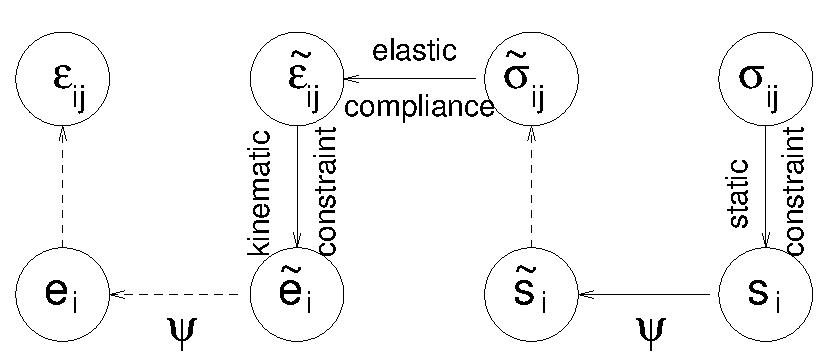
\includegraphics[width=0.8\textwidth]{dm_comp.eps}}
\end{htmlonly}
%begin{latexonly}
 \centerline{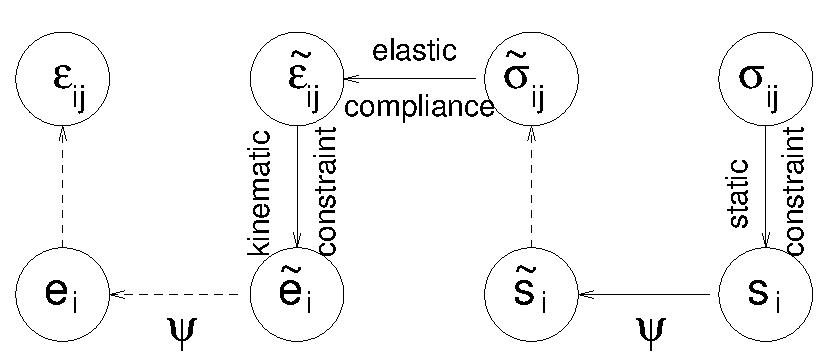
\includegraphics[width=0.7\textwidth]{dm_comp}}
%end{latexonly}
\caption{Structure of microplane-based anisotropic damage model}
\label{ff4}
\end{figure}

Combining the basic equations, it is possible to show that the
components of the damaged
material compliance tensor are given by
\begin{equation}
\label{damcom}
C_{ijkl}=M_{pqij}M_{rskl}C^e_{pqrs}
\end{equation}
where $C^e_{pqrs}$ are the components of the elastic material compliance tensor,
\begin{equation}
\label{ee27}
M_{ijkl} = \quarter\left(
\psi_{ik}\delta_{jl}+\psi_{il}\delta_{jk}+\psi_{jk}\delta_{il}+\psi_{jl}\delta_{ik}\right)
\end{equation}
are the components of the so-called damage effect tensor, and
\begin{equation}
\label{ee24}
\psi_{ij} = \frac{3}{2\pi}\int_\Omega \psi\, n_i n_j \dO
\end{equation}
are the components of the second-order inverse integrity tensor.
The integration domain $\Omega$ is the unit hemisphere.
In practice, the integral over the unit hemisphere is evaluated by
summing the contribution from a finite number of directions, according
to one of the numerical integration schemes that are used by microplane
models.

The scalar variable $\psi$ characterizes the relative compliance
in the direction given by the vector $\mbf{n}$.
If $\psi$ is the same in all directions,
the inverse integrity tensor  evaluated from (\ref{ee24})
is equal to the unit second-order tensor (Kronecker delta) multiplied
by $\psi$, the damage effect tensor evaluated from (\ref{ee27})
is equal to the symmetric fourth-order unit tensor multiplied
by $\psi$,
and the damaged
material compliance tensor evaluated from (\ref{damcom}) is the
elastic compliance tensor multiplied by $\psi^2$. The factor multiplying
the elastic compliance tensor in the
isotropic damage model is $1/(1-\omega)$, and so $\psi$ corresponds
to  $1/\sqrt{1-\omega}$. In the initial undamaged state,
$\psi=1$ in all directions.  The evolution of $\psi$
is governed by the history of the projected strain components.
In the simplest case, $\psi$ is driven by the normal strain
$e_N=\eps_{ij}n_in_j$. Analogy with the isotropic damage model
leads to the damage law
\begin{equation}
\psi=f(\kappa)
\end{equation}
and loading-unloading conditions
\begin{equation}
g(e_N,\kappa)\equiv e_N-\kappa\le 0, \hskip 10mm
\dot{\kappa}\ge 0, \hskip 10mm
\dot{\kappa}g(e_N,\kappa)=0
\end{equation}
in which $\kappa$ is a history variable that represents the maximum
level of normal strain in the given direction ever reached in the
previous history of the material. An appropriate modification
of the exponential softening
law leads to the damage law
\begin{equation}
\label{expsoft2}
f(\kappa)=\left\{
\begin{array}{ll}
1 & \mbox{ if } \kappa\le e_0
\\
\sqrt{\frac{\kappa}{e_0}\exp\left(\frac{\kappa-e_0}{e_f-e_0}\right)}
& \mbox{ if } \kappa>e_0
\end{array}
\right.
\end{equation}
where $e_0$ is a parameter controlling the elastic limit, and $e_f>e_0$
is another parameter controlling ductility.
Note that softening in a limited number of directions does not necessarily
lead to softening on the macroscopic level, because the response
in the other directions remains elastic. Therefore, $e_0$ corresponds
to the elastic limit but not to the state at peak stress.

If the MDM model is used in its basic form described above,
the compressive strength turns out to depend on the Poisson ratio and,
in applications to concrete, its value is too low compared to the
tensile strength. The model is designed primarily for tensile-dominated
failure, so the low compressive strength
is not considered as a major drawback. Still, it
is desirable to introduce a modification that would prevent spurious
compressive failure in problems where moderate compressive stresses
appear. The desired effect is achieved by redefining the projected
strain $e_N$ as
\begin{equation}
\label{ee37}
e_N =  \frac{\eps_{ij}n_in_j}{1-\displaystyle\frac{m}{Ee_0}\sigma_{kk}}
\end{equation}
where $m$ is a nonnegative parameter that controls the sensitivity to the
mean stress, $\sigma_{kk}$ is the trace of the stress tensor,
and the normalizing factor
$Ee_0$ is introduced in order to render the parameter
$m$ dimensionless.
Under compressive stress states (characterized by $\sigma_{kk}<0$),
the denominator in (\ref{ee37}) is larger than 1, and the projected strain
is reduced, which also leads to a reduction of damage.
A typical recommended value of parameter $m$ is 0.05.

\paragraph{Nonlocal formulation}

Nonlocal formulation of the MDM model is based on the averaging of
the inverse integrity tensor. This roughly corresponds to the nonlocal
isotropic damage model with averaging of the compliance variable
$\gamma=\omega/(1-\omega)$, which does not cause any spurious locking effects.
In equation (\ref{ee27}) for the evaluation of the damage effect tensor,
the inverse integrity tensor is replaced by its weighted average with
components
\begin{equation}
\label{psinl1}
\bar{\psi}_{ij}(\vx)=\int_V \alpha(\vx,\vxi)\psi_{ij}(\vxi)\mbox{d}\vxi
\end{equation}

By fitting a wide range of numerical results, it has been found that
the parameters of the nonlocal MDM model can be estimated from the
measurable material properties using the formulas
\begin{eqnarray}
\lambda_f&=&\frac{EG_f}{Rf_t^2}
\\
\lambda&=&\frac{\lambda_f}{1.47-0.0014\lambda_f}
\\
e_0&=&\frac{f_t}{(1-m)E(1.56+0.006\lambda)}
\\
e_f&=&e_0[1+(1-m)\lambda]
\end{eqnarray}
where $E$ is Young's modulus, $G_f$ is the fracture energy, $f_t$
is the uniaxial tensile strength,
$m$ is the compressive correction factor, typically chosen
as $m=0.05$, and $R$ is the radius of nonlocal interaction reflecting the
internal length of the material.
\paragraph{Input Record}
The model description and parameters are summarized
in Tab.~\ref{mdm_table}.

\begin{table}[!htb]
%\begin{center}
\begin{tabular}{|l|p{9cm}|}
\hline
Description & MDM Anisotropic damage model\\
\hline
& Common parameters\\
Record Format & \descitem{Mdm} \elemparam{d}{rn} \elemparam{nmp}{ins} \elemparam{talpha}{rn}
\elemparam{parmd}{rn}  \elemparam{nonloc}{in}
\elemparam{formulation}{in} \elemparam{mode}{in}\\
Parameters & -\param{num} material model number\\
& - \param{D} material density\\
& - \param{nmp} number of microplanes used for hemisphere integration,
supported values are 21,28, and 61\\
& - \param{talpha}  thermal dillatation coeff\\
& - \param{parmd} \\
& - \param{nonloc} \\
& - \param{formulation}\\
& - \param{mode}\\
\hline
Nonlocal variant I&\\
Additional params &\elemparam{r}{rn} \elemparam{efp}{rn}
\elemparam{ep}{rn} \\
& -\param{r} nonlocal interaction radius\\
& -\param{efp} $\varepsilon_fp$ is a model parameter that controls
the post-peak slope $\varepsilon_fp$ =$\varepsilon_f-\varepsilon_0$,
where $\varepsilon_f$ is strain at zero stress level.\\
& -\param{ep} max effective strain at peak $\varepsilon_0$\\
\hline
Nonlocal variant II&\\
Additional params &\elemparam{r}{rn} \elemparam{gf}{rn}
\elemparam{ft}{rn}\\
& -\param{r} nonlocal intraction radius\\
& -\param{gf} fracture energy\\
& -\param{ft} tensile strength\\
\hline
Local variant I&\\
Additional params &\elemparam{efp}{rn} \elemparam{ep}{rn}\\
& -\param{efp} $\varepsilon_fp$ is a model parameter that controls
the post-peak slope $\varepsilon_fp$ =$\varepsilon_f-\varepsilon_0$,
where $\varepsilon_f$ is strain at zero stress level.\\
& -\param{ep} max effective strain at peak $\varepsilon_0$\\
\hline
Local variant II&\\
Additional params &\elemparam{gf}{rn} \elemparam{ep}{rn}\\
& -\param{gf} fracture energy\\
& -\param{ep} max effective strain at peak $\varepsilon_0$\\
\hline
Supported modes& 3dMat, PlaneStress\\
Features & Adaptivity support\\
\hline
\end{tabular}
\caption{MDM model - summary.}
\label{mdm_table}
%\end{center}
\end{table}

\clearpage
\subsubsection{Isotropic damage model for interfaces}
\label{sec:idmfi}

The model provides an interface law, which can be used to describe a damageable interface between two materials (e.g.\ between steel reinforcement and concrete). The law is formulated in terms of the traction vector and the displacement jump vector. The basic response is elastic, with stiffness \param{kn} in 
the normal direction and \param{ks} in the tangential direction.
Similar to other isotropic damage models, this model assumes that the stiffness degradation is isotropic, i.e., both stiffness moduli decrease proportionally and independently of the loading 
direction. The damaged stiffnesses are \param{kn}$\times\omega$ and \param{ks}$\times\omega$ where $\omega$ is a scalar damage variable.
The damage evolution law is postulated in an explicit form, relating
the damage variable $\omega$ to the largest previously reached 
equivalent ``strain'' level, $\kappa$.

The equivalent ``strain'', $\tilde\varepsilon$, is a scalar measure derived from the displacement jump vector. The choice of the specific expression
for the equivalent strain affects the shape of the elastic domain
in the strain space and plays a similar role to the choice of a yield
condition in plasticity.
Currently, in the present implementation,  $\tilde\varepsilon$ is equal to the positive part of the normal diplacement jump (opening of the interface).
Only the exponential softening damage law is supported:
$$
\omega = 1 - \frac{\varepsilon_0}{\kappa}  \exp\left( - \frac{f_t( \kappa - \varepsilon_0 )}{G_f} \right)
$$
The model parameters are summarized in Tab.~\ref{iid_table}. 
\begin{table}[!htb]
%\begin{center}
  \small
\begin{tabular}{|l|p{9cm}|}
\hline
Description & Isotropic damage model for concrete in tension\\
\hline
Record Format & \descitem{isointrfdm01} 
\elemparam{kn}{rn} \elemparam{ks}{rn} \elemparam{ft}{rn} \elemparam{gf}{rn} \optelemparam{maxomega}{rn} \elemparam{talpha}{rn} \elemparam{d}{rn}\\
Parameters & - \param{d} material density\\
&- \param{tAlpha} thermal dilatation coefficient\\
&- \param{kn} elastic stifness in normal direction\\
&- \param{ks} elastic stifness in tangential direction\\
&- \param{ft} tensile strength\\
&- \param{gf} fracture energy\\
&- \param{maxomega} maximum damage, used for convergence improvement
(its value is between 0 and 0.999999 (default), 
and it affects only the secant stiffness but not the stress)\\
Supported modes& 2dInterface, 3dInterface\\
Features & \\
\hline
\end{tabular}
\caption{Isotropic damage model for interface elements -- summary.}
\label{iid_table}
%\end{center}
\end{table}


\subsection{Material models specific to concrete}
\subsubsection{Mazars damage model for concrete - MazarsModel}
This isotropic damage model assumes that the stiffness degradation is
isotropic, i.e., stiffness moduli corresponding to different
directions decrease proportionally and independently of direction of
loading.
It introduces two damage parameters $\omega_t$ and $\omega_c$ that
are computed from the same equivalent strain using two different damage functions
$g_t$ and $g_c$. The $g_t$ is identified from the uniaxial tension tests, while
$g_c$ from compressive test. The damage parameter for general stress states
$\omega$ is obtained as a linear combination of $\omega_t$ and $\omega_c$:
$\omega=\alpha_t g_t + \alpha_c g_c$, where the coefficients
$\alpha_t$ and $\alpha_c$ take into account the character of the
stress state.
The damaged stiffness tensor is expressed as
$\mbf{D}=(1-\omega)\mbf{D}^e$.
Damage evolution law is postulated in an explicit form, relating
damage parameter and scalar measure of largest reached strain level in
material, taking into account the principle of preserving of fracture
energy $G_f$. The equivalent strain, i.e., a scalar measure of the
strain level is defined as norm from positive principal strains.
The model description and parameters are summarized
in Tab.~\ref{maz_table}.


\begin{table}[!htb]
%\begin{center}
\begin{tabular}{|l|p{9cm}|}
\hline
Description & Mazars damage model for concrete\\
\hline
Record Format & \descitem{MazarsModel} \elemparam{d}{rn} \elemparam{E}{rn}
\elemparam{n}{rn}  \elemparam{e0}{rn}
\elemparam{ac}{rn} [\elemparam{bc}{rn}] [\elemparam{beta}{rn}]
\elemparam{at}{rn} \optelemparam{bt}{rn}
[\elemparam{hreft}{rn}] [\elemparam{hrefc}{rn}]
[\elemparam{version}{in}] [\elemparam{tAlpha}{rn}] [\elemparam{equivstraintype}{in}]
[\elemparam{maxOmega}{rn}]\\
Parameters &- \param{num} material model number\\
&- \param{d} material density\\
&- \param{E} Young modulus\\
&- \param{n} Poisson ratio\\
&- \param{e0} max effective strain at peak\\
&- \param{ac},\param{bc} material parameters related to the shape of
uniaxial compression curve (A sample set used by Saouridis is $A_c =
1.34, B_c = 2537$\\
&- \param{beta} coefficient reducing the effect of damage under
response under shear. Default value set to 1.06\\
&- \param{at}, \optparam{bt} material parameters related to the shape of
uniaxial tension curve. Meaning dependent on \param{version}
parameter.\\
&- \param{hreft}, \param{hrefc} reference characteristic lengths for
tension and compression. The material parameters are specified for
element with these characteristic lengths. The current element then
will have the same COD (Crack Opening Displacement) as reference one.\\
&- \param{version} Model variant. if 0 specified, the original form
$g_t= 1.0-(1.0-A_t)*\varepsilon_0/\kappa - A_t*\exp(-B_t*(\kappa-\varepsilon_0));
$ of
tension damage evolution law is used, if equal 1, the modified law
used which asymptotically tends to zero
$g_t = 1.0-(\varepsilon_0/\kappa)*\exp((\varepsilon_0-\kappa)/A_t)$\\
&- \param{tAlpha} thermal dilatation coefficient\\
&- \param{equivstraintype} see Tab.~\ref{id_table}\\
&- \param{maxOmega} limit maximum damage, use for convergency improvement\\
Supported modes& 3dMat, PlaneStress, PlaneStrain, 1dMat\\
\hline
\end{tabular}
\caption{Mazars damage model  -- summary.}
\label{maz_table}
%\end{center}
\end{table}


\subsubsection{Nonlocal Mazars damage model for concrete - MazarsModelnl}
The nonlocal variant of Mazars damage model for concrete.
Model based on nonlocal averaging of equivalent strain.
The nonlocal averaging acts as a powerful localization
limiter. The bell-shaped nonlocal averaging function is used.
The model description and parameters are summarized
in Tab.~\ref{maznl_table}.

\begin{table}[!htb]
%\begin{center}
\begin{tabular}{|l|p{9cm}|}
\hline
Description & Nonlocal Mazars damage model for concrete\\
\hline
Record Format & \descitem{MazarsModelnl} \elemparam{r}{rn} \elemparam{E}{rn}
\elemparam{n}{rn}  \elemparam{e0}{rn}
\elemparam{ac}{rn} \elemparam{bc}{rn} \elemparam{beta}{rn}
\elemparam{version}{in} \elemparam{at}{rn} \optelemparam{bt}{rn} \elemparam{r}{rn}
\elemparam{tAlpha}{rn} \\
Parameters &- \param{num} material model number\\
&- \param{d} material density\\
&- \param{E} Young modulus\\
&- \param{n} Poisson ratio\\
&- \param{maxOmega} limit maximum damage, use for convergency improvement\\
&- \param{tAlpha} thermal dilatation coefficient\\
&- \param{version} Model variant. if 0 specified, the original form
$g_t= 1.0-(1.0-A_t)*\varepsilon_0/\kappa - A_t*\exp(-B_t*(\kappa-\varepsilon_0));
$ of
tension damage evolution law is used, if equal 1, the modified law
used which asymptotically tends to zero
$g_t = 1.0-(\varepsilon_0/\kappa)*\exp((\varepsilon_0-\kappa)/A_t)$\\
&- \param{ac},\param{bc} material parameters related to the shape of
uniaxial compression curve (A sample set used by Saouridis is $A_c =
1.34, B_c = 2537$\\
&- \param{at}, \optparam{bt} material parameters related to the shape of
uniaxial tension curve. Meaning dependent on \param{version}
parameter.\\
&- \param{beta} coefficient reducing the effect of damage under
response under shear. Default value set to 1.06\\
&- \param{r} parameter specifying the width of nonlocal averaging zone\\
Supported modes& 3dMat, PlaneStress, PlaneStrain, 1dMat\\
\hline
\end{tabular}
\caption{Nonlocal Mazars damage model  -- summary.}
\label{maznl_table}
%\end{center}
\end{table}


\subsubsection{CebFip78 model for concrete creep with aging - CebFip78}
Implementation of aging viscoelastic model for concrete creep
according to the CEB-FIP Model Code.
The model parameters are summarized
in Tab.~\ref{cebfip_table}.

\begin{table}[!htb]
%\begin{center}
\begin{tabular}{|l|p{9cm}|}
\hline
Description & CebFip78 model  for concrete creep with aging\\
\hline
Record Format & \descitem{CebFip78}  \elemparam{n}{rn}
\elemparam{relMatAge}{rn} \elemparam{E28}{rn} \elemparam{fibf}{rn} \elemparam{kap\_a}{rn}
\elemparam{kap\_c}{rn} \elemparam{kap\_tt}{rn} \elemparam{u}{rn}\\
Parameters &- \param{num} material model number\\
&- \param{E28} Young modulus at age of 28 days [MPa]\\
&- \param{n} Poisson ratio\\
&- \param{fibf} basic creep coefficient\\
&- \param{kap\_a} coefficient of hydrometric conditions\\
&- \param{kap\_c} coefficient of type of cement\\
&- \param{kap\_tt} coeficient of temperature effects\\
&- \param{u} surface imposed to environment [$mm^2$]; temporary here; should be in crosssection level\\
&- \param{relmatage} relative material age \\
Supported modes& 3dMat, PlaneStress, PlaneStrain, 1dMat,
2dPlateLayer,2dBeamLayer, 3dShellLayer\\
\hline
\end{tabular}
\caption{CebFip78 material model -- summary.}
\label{cebfip_table}
%\end{center}
\end{table}



\subsubsection{Double-power law model for concrete creep with aging - DoublePowerLaw}
Implementation of aging viscoelastic model for concrete creep
with compliance function given by the double-power law.
The model parameters are summarized
in Tab.~\ref{doublepowerlaw_table}.

\begin{table}[!htb]
%\begin{center}
\begin{tabular}{|l|p{9cm}|}
\hline
Description & Double-power law model  for concrete creep with aging\\
\hline
Record Format & \descitem{DoublePowerLaw}  \elemparam{n}{rn}
\elemparam{relMatAge}{rn} \elemparam{E28}{rn} \elemparam{fi1}{rn} \elemparam{m}{rn}
\elemparam{n}{rn} \elemparam{alpha}{rn} \\
Parameters &- \param{num} material model number\\
&- \param{E28} Young modulus at age of 28 days [MPa]\\
&- \param{n} Poisson ratio\\
&- \param{fibf} basic creep coefficient\\
&- \param{m} coefficient \\
&- \param{n} coefficient \\
&- \param{alpha} coeficient \\
&- \param{relmatage} relative material age \\
Supported modes& 3dMat, PlaneStress, PlaneStrain, 1dMat,
2dPlateLayer,2dBeamLayer, 3dShellLayer\\
\hline
\end{tabular}
\caption{Double-power law model -- summary.}
\label{doublepowerlaw_table}
%\end{center}
\end{table}

\subsubsection{B3 and MPS models for concrete creep with aging}

Model B3 is an aging viscoelastic model for concrete creep and shrinkage, developed by Prof. Ba\v{z}ant and coworkers. In OOFEM it is implemented in three different ways. 

The first version, ``B3mat'', is kept in OOFEM for compatibility. It is based on an aging Maxwell chain. The moduli of individual units in the chain are evaluated in each step using the least-squares method.

The second, more recent version, is referred to as ``B3solidmat''. Depending on the specified input it exploits either a non-aging Kelvin chain combined with the solidification theory, or an aging Kelvin chain. It is extended to the so-called microprestress-solidification theory (MPS), which in this implementation  takes into account only the effects of variable humidity on creep; the effects of temperature on creep are not considered. 
The underlying rheological chain consists of four serially coupled components. The solidifying Kelvin chain represents short-term creep; it is serially coupled with a non-aging elastic spring that reflects instantaneous deformation. Long-term creep is captured by an aging dashpot with viscosity dependent on the microprestress, the evolution of which is affected by changes of humidity. The last  unit describes volumetric deformations (shrinkage and thermal strains).
Drying creep is incorporated either by the 
``averaged cross-sectional approach'', or by the ``point approach''.

%%%% MPS
The latest version is denoted as ``MPS'' and is based on the microprestress-solidification theory. The rheological model consists of the same four components as in  ``B3solidmat'', but now the implemented exponential algorithm is designed especially for the solidifying Kelvin chain, which is a special case of an aging Kelvin chain. This model takes into account both humidity and temperature effects on creep. Drying creep is incorporated exclusively by the so-called
``point approach''. The model can operate in two modes,
controlled by the keyword $CoupledAnalysisType$. The first mode ($CoupledAnalysisType = 0$) solves only the basic creep and runs as a single problem, while the second mode ($CoupledAnalysisType = 1$) needs to be run as a staggered problem with humidity and temperature analysis preceding the mechanical problem.

The basic creep is in the microprestress-solidification theory influenced by the same four parameters $q_1$ - $q_4$ as in the model B3. Values of these parameters can be estimated from the composition of concrete mixture and its compressive strength using the following empirical formulae: 
\begin{eqnarray}
  q_1 &=& 126.77 \bar{f_c}^{-0.5} \hspace{5 mm} [10^{-6}/\mbox {MPa}]\\
  q_2 &=& 185.4 c^{0.5} \bar{f_c}^{-0.9} \hspace{5 mm} [10^{-6}/\mbox {MPa}]\\
  q_3 &=& 0.29 \left(w/c\right)^4 q_2 \hspace{5 mm} [10^{-6}/\mbox {MPa}]\\
  q_4 &=& 20.3 \left(a/c\right)^{-0.7} \hspace{5 mm} [10^{-6}/\mbox {MPa}]  
\end{eqnarray}
Here, $\bar{f_c}$ is the average compressive cylinder strength at age of 28 days [MPa], $a$, $w$ and $c$ is the weight  of aggregates, water and cement per unit volume of concrete [kg/m$^3$].

%%%%     SPRING %%%%
The non-aging spring stiffness represents the asymptotic modulus of the material; it is equal to $1/q_1$.
%%%%     KELIVIN CHAIN %%%%
The solidifying Kelvin chain is composed of $M$ Kelvin units with fixed retardation times $\tau_{\mu}$, $\mu = 1, 2, \dots, M$, which form a geometric progression with quotient 10. The lowest retardation time $\tau_1$ is equal to $0.3\; begoftimeofinterest$, the highest retardation time $\tau_M$ is bigger than $0.5\; endoftimeofinterest$. The chain also contains a spring with stiffness $E_0^\infty$
(a special case of Kelvin unit with zero retardation time).
Moduli $E_{\mu}^\infty$ of individual Kelvin units are determined such that the chain
provides a good approximation of the non-aging micro-compliance function of the solidifying constituent, $\Phi(t-t') = q_2 \ln \left( 1 + \left( \left(t-t' \right)/\lambda_0 \right)^n \right)$, where $\lambda_0 = 1$ day and $n = 0.1$. 
The technique based on the continuous retardation spectrum
leads to the following formulae:
\begin{eqnarray}
 \frac{1}{E_0^\infty} &=& q_2 \ln\left(1+\tilde{\tau_0}\right) - \frac{q_2 \tilde{\tau_0} }{10 \left( 1 + \tilde{\tau_0} \right)} \hspace{5 mm} \mbox{ where} \hspace{5 mm} \tilde{\tau_0} = \left( \frac{2 \tau_1}{ \sqrt{10}}  \right)^{0.1} \\
\frac{1}{E_\mu^\infty} &=&  (\ln 10) \frac{q_2 \tilde{\tau}_\mu \left(0.9 + \tilde{\tau}_\mu \right)}{10 \left( 1 + \tilde{\tau}_\mu \right)^2} \hspace{5 mm} \mbox{ where} \hspace{5 mm} \tilde{\tau}_\mu = \left(2 \tau_\mu \right)^{0.1}, \hspace{7 mm} \mu = 1,2,\dots M
\end{eqnarray}
Viscosities $\eta_{\mu}^\infty$ of individual Kelvin units are obtained from simple relation $\eta_{\mu}^\infty=\tau_{\mu}/E_{\mu}^\infty$. A higher accuracy is reached if all retardation times are in the end multiplied by the factor 1.35 and the last modulus $E_M$ is divided by 1.2.

%%%%     SOLIDIFICATION %%%%
The actual viscosities $\eta_{\mu}$ and stiffnesses $E_{\mu}$ of the solidifying chain change in time according to $\eta_{\mu}(t) = v(t) \eta_{\mu}^\infty$ and $E_{\mu}(t) = v(t) E_{\mu}^\infty$, where 
\begin{equation}
v(t)= \frac{1}{\frac{q_3}{q_2} + \left( \frac{\lambda_0}{ t} \right)^m}
\end{equation}
is the volume growth function, and exponent $m = 0.5$. In the case of variable temperature or humidity, the actual age of concrete 
$t$ is replaced by the equivalent time $t_e$, which is obtained by integrating
(\ref{dtedt}).

%%%%     MICROPRESTRESS %%%%
Evolution of viscosity of the aging dashpot is governed by the differential
equation 
\begin{equation}
\label{eq:mps_viscosity}
\dot{\eta}+\frac{1}{\mu_S T_0} \left |  T \frac{\dot{h}}{h} - \kappa_T k_T(T) \dot{T}  \right | \left( \mu_S \eta \right)^{p/\left(p-1\right)} = \frac{\psi_S}{q_4}
\end{equation}
where $h$ is the relative pore humidity, $T$ is the absolute temperature [K], $T_0 = 298$ K is the room temperature,  and parameter $p = 2$. 
Function $k_T$ is given by 
\begin{equation}
\quad k_T(T) = \mbox{e}^{-c_T \left (T_{max}-T\right )}
\label{eq:mps_k_T}
\end{equation}
where parameter $c_T$ controls the influence of cyclic temperature on creep, and $T_{max}$ stands for the maximum reached temperature in the previous history. 
This is a modification of the opriginal MPS theory, proposed by Havl\'{a}sek and Jir\'{a}sek. 
%Parameter $\kappa_T$ replaces $\ln h$ which in case of basic creep eliminates the sensitivity of the original model on the choice of relative pore humidity $h$ reached by self-desicca.


Equation (\ref{eq:mps_viscosity}) differs from the one presented in the original work; it replaces the differential equation for microprestress, which is not used here. The evolution of viscosity can be captured directly, without the need for microprestress. What matters is only the relative humidity and temperature and their rates. Parameters $c_0$ and $k_1$ of the original MPS theory
are replaced by $\mu_S = c_0 T_0^{p-1} k_1^{p-1} q_4 (p-1)^p$. 
The initial value of viscosity is defined as $\eta(t_0) = t_0/q_4$, where $t_0$ is age of concrete at the onset drying or when the temperature starts changing.



%%%%     MODIFIED TIMES %%%%
As mentioned above, under variable humidity and temperature conditions the physical time $t$ in function $v(t)$ describing evolution of the solidified volume is replaced by the equivalent time $t_e$. In a similar spirit, $t$ is replaced by the solidification time $t_s$ in the equation describing creep of the solidifying constituent, and by the reduced time $t_r$ in equation $\mbox{d} \varepsilon_f / \mbox{d} t_r = \sigma / \eta(t)$ relating the flow strain rate to the stress.
Factors transforming the physical time $t$ into $t_e$, $t_r$ and $t_s$ are defined as follows:
\begin{eqnarray}
\label{dtedt}
 \frac{dt_e}{dt} &=& \psi_e(t) = \beta_{eT}(T(t))\, \beta_{eh}(h(t))\\
 \frac{dt_r}{dt} &=& \psi_r(t) = \beta_{rT}(T(t))\, \beta_{rh}(h(t))\\
 \frac{dt_s}{dt} &=& \psi_s(t) = \beta_{sT}(T(t))\, \beta_{sh}(h(t))
\end{eqnarray}
Functions describing the influence of temperature have the form 
\begin{eqnarray}
 \beta_{eT}(T) &=& \exp \left[ \frac{Q_e}{R}\left( \frac{1}{T_0} - \frac{1}{T} \right) \right]\\
 \beta_{rT}(T) &=& \exp \left[ \frac{Q_r}{R}\left( \frac{1}{T_0} - \frac{1}{T} \right) \right]\\
 \beta_{sT}(T) &=& \exp \left[ \frac{Q_s}{R}\left( \frac{1}{T_0} - \frac{1}{T} \right) \right]
\end{eqnarray}
motivated by the rate process theory.
$R$ is the universal gas constant and $Q_e$, $Q_r$, $Q_s$ are activation energies for hydration, viscous processes and microprestress relaxation, respectively.
Only the ratios $Q_e/R$, $Q_r/R$ and $Q_s/R$ have to be specified.
Functions describing the influence of humidity have the form 
\begin{eqnarray}
 \beta_{eh}(h) &=& \frac{1}{1+\left[\alpha_e \left( 1-h\right) \right]^4}\\
 \beta_{rh}(h) &=& \alpha_r + \left( 1 - \alpha_r \right) h^2\\
 \beta_{sh}(h) &=& \alpha_s + \left( 1 - \alpha_s \right) h^2
\end{eqnarray}
where $\alpha_e$, $\alpha_r$ and $\alpha_s$ are parameters. 

%%%%     HYGRO AND THERMAL STRAIN  %%%%
The rate of thermal strain is expressed as $\dot{\varepsilon}_T = \alpha_T \dot{T}$ and the rate of shrinkage strain as $\dot{\varepsilon}_{sh} = k_{sh} \dot{h}$, where both $\alpha_T$ and $k_{sh}$ are assumed to be constant in time and independent of temperature and humidity. 




The model description and parameters are summarized
in Tab.~\ref{b3_table} for ``B3mat'', in Tab.~\ref{b3solid_table} for ``B3solidmat'', and in Tab.~\ref{mps_table} for ``MPS''. 
Since some model parameters are determined from the composition
and strength using empirical formulae, it is necessary to use the
specified units (e.g.\ compressive strength always in MPa, irrespectively
of the units used in the simulation for stress). 
For ``B3mat'' and ``B3solidmat'' it is strictly 
required to use the specified units in the material input record (stress always in MPa, time in days etc.). 
The ``MPS'' model is almost unit-independent, except for 
$\bar{f}_c$ in MPa and $c$ in kg/m$^3$, which are used in empirical formulae.

%%%%%%%% B3 MAT %%%%%%%%%

\begin{table}[!htb]
%\begin{center}
\begin{tabular}{|l|p{9cm}|}
\hline
Description & B3 material model  for concrete aging\\
\hline
Record Format & \descitem{B3mat}  \elemparam{d}{rn} \elemparam{n}{rn}
\elemparam{talpha}{rn} 
%for rheo chain material
\optelemparam{begoftimeofinterest}{rn} \optelemparam{endoftimeofinterest}{rn} \elemparam{timefactor}{rn} \elemparam{relMatAge}{rn}
%
\optelemparam{mode}{in} 
% mode = 0
\elemparam{fc}{rn} \elemparam{cc}{rn} \elemparam{w/c}{rn}
\elemparam{a/c}{rn} \elemparam{t0}{rn}
% mode = 1
\elemparam{q1}{rn} \elemparam{q2}{rn} \elemparam{q3}{rn}
\elemparam{q4}{rn}
%
\elemparam{shmode}{in}
% shmode 1
\elemparam{ks}{rn} \elemparam{vs}{rn} \elemparam{hum}{rn}
%% mode 0
\optelemparam{alpha1}{rn} \optelemparam{alpha2}{rn} 
%% mode 1
\elemparam{kt}{rn} \elemparam{EpsSinf}{rn} \elemparam{q5}{rn}
% shmode 2
\elemparam{es0}{rn} \elemparam{r}{rn} \elemparam{rprime}{rn}
\elemparam{at}{rn}  
\elemparam{w\_h}{rn} \elemparam{ncoeff}{rn} \elemparam{a}{rn}
\\
Parameters &- \param{num} material model number\\
%
&- \param{d} material density\\
&- \param{n} Poisson ratio\\
&- \param{talpha} coefficient of thermal expansion\\
&- \param{begoftimeofinterest} optional parameter; lower boundary of
time interval with good approximation of the compliance function
[day]; default 0.1 day\\
&- \param{endoftimeofinterest} optional parameter; upper boundary of
time interval with good approximation of the compliance function
[day]\\
&- \param{timefactor} scaling factor transforming the simulation time units into days\\
&- \param{relMatAge} relative material age [day]\\
%
&- \param{mode} if $mode = 0$ (default value) creep and shrinkage parameters are
predicted from composition; for $mode = 1$ parameters must be user-specified.\\
&- \param{fc} 28-day mean cylinder compression strength [MPa]\\
&- \param{cc} cement content of concrete [kg/m$^{3}$]\\
&- \param{w/c} ratio (by weight) of water to cementitious material\\
&- \param{a/c} ratio (by weight) of aggregate to cement \\
&- \param{t0} age when drying begins [day]\\
&- \param{q1-q4} parameters of B3 model for basic creep [1/TPa]\\
%
&- \param{shmode} shrinkage mode;
$0=$ no shrinkage;
$1=$ average shrinkage (the following parameters must be specified:
\param{ks}, \param{vs}, \param{hum} and additionally  \param{alpha1} \param{alpha2} for $mode = 0$
and \param{kt} \param{EpsSinf} \param{q5} \param{t0} for $mode = 1$;  
$2=$ point shrinkage (needed: \param{es0}, \param{r}, \param{rprime},
\param{at}, \param{w\_h}, \param{ncoeff}, \param{a})\\
%
&- \param{ks} cross-section shape factor [-]\\
&- \param{vs} volume to surface ratio [m]\\
&- \param{hum} relative humidity of the environment [-]\\
&- \param{alpha1} shrinkage parameter -- influence of cement type [-]\\
&- \param{alpha2} shrinkage parameter -- influence of curing type [-]\\
&- \param{kt} shrinkage parameter [day/m$^2$]\\
&- \param{EpsSinf} shrinkage parameter [10$^{-6}$]\\
&- \param{q5} drying creep parameter [1/TPa]\\
%
&- \param{es0} final shrinkage at material point\\
&- \param{r}, \param{rprime} coefficients\\
&- \param{at} oefficient relating stress-induced thermal strain and shrinkage\\
&- \param{w\_h}, \param{ncoeff}, \param{a} sorption isotherm parameters obtained from experiments [Pedersen, 1990] \\
%
Supported modes& 3dMat, PlaneStress, PlaneStrain, 1dMat,
2dPlateLayer,2dBeamLayer, 3dShellLayer\\
\hline
\end{tabular}
\caption{B3 creep and shrinkage model -- summary.}
\label{b3_table}
%\end{center}
\end{table}

For illustration, sample input records for the material considered in Example 3.1 of the creep
book by Ba\v{z}ant and Jir\'{a}sek is presented. The concrete mix is composed
of 170 kg/m$^3$ of water, 450 kg/m$^3$ of type-I cement and 1800 kg/m$^3$ of aggregates,
which corresponds to ratios $w/c=0.3778$ and $a/c=4$. The compressive strength 
is $\bar{f}_c=45.4$ MPa. The concrete slab of thickness 200 mm is cured in air
with initial protection against drying until the age of 7 days.
Subsequently, the slab is exposed to an environment with
relative humidity of 70\%. The following input record can be used for the first
version of the model (B3mat):

{\tt B3mat 1 n 0.2 d 0. talpha 1.2e-5 relMatAge 28. fc 45.4 cc 450. w/c 0.3778 a/c 4. t0 7. timefactor 1. alpha1 1. alpha2 1.2 ks 1. hum 0.7 vs 0.1 shmode 1}

Parameter $\alpha_1=1$ corresponds to type-I cement, parameter $\alpha_2=1.2$
to curing in air, parameter $k_s=1$ to an infinite slab. 
The volume-to-surface ratio is in this case 
equal to one half of the slab thickness
and must be specified in meters, independently of the length units that are
used in the finite element analysis (e.g., for nodal coordinates).
The value of relMatAge must be specified in days.
Parameter {\tt relMatAge 28.}  means that time 0
of the analysis corresponds to concrete age 28 days. 
If material B3mat is used, the finite element analysis
must use days as the units of time (not only for relMatAge,
but in general, e.g.\ for the time increments).

If only the basic creep (without shrinkage) should be computed, then
the material input record reduces to following:
{\tt B3mat 1 n 0.2 d 0. talpha 1.2e-5 relMatAge 28. fc 45.4 cc 450. w/c 0.3778 a/c 4. t0 7. timefactor 1. shmode 0}



%%%%%%%% B3 SOLID MAT %%%%%%%%%

\begin{table}[!htb]
\begin{tabular}{|l|p{9cm}|}
\hline
Description & B3solid material model  for concrete creep\\
\hline
Record Format & \descitem{B3solidmat} 
\elemparam{d}{rn} \elemparam{n}{rn} \elemparam{talpha}{rn}
%
\elemparam{mode}{in} 
\optelemparam{EmoduliMode}{in} 
\elemparam{Microprestress}{in}
\elemparam{shm}{in} 
%for rheo chain material
\optelemparam{begoftimeofinterest}{rn} \optelemparam{endoftimeofinterest}{rn} \elemparam{timefactor}{rn} \elemparam{relMatAge}{rn}
\elemparam{fc}{rn} \elemparam{cc}{rn} \elemparam{w/c}{rn} \elemparam{a/c}{rn} \elemparam{t0}{rn} % mode = 0 
\elemparam{q1}{rn} \elemparam{q2}{rn} \elemparam{q3}{rn} \elemparam{q4}{rn} % mode = 1
%
\elemparam{c0}{rn} \elemparam{c1}{rn} \elemparam{tS0}{rn} %MPS = 1
\elemparam{w\_h}{rn} \elemparam{ncoeff}{rn} \elemparam{a}{rn}
%
%shm = 1 B3_AverageShrinkage
\elemparam{ks}{rn} 
%for shm = 1 and mode = 0            
\optelemparam{alpha1}{rn} \optelemparam{alpha2}{rn} \elemparam{hum}{rn} \elemparam{vs}{rn}
%for shm = 1 and mode = 1
\elemparam{q5}{rn} \elemparam{kt}{rn} \elemparam{EpsSinf}{rn}
% = 2 B3_PointShrinkage
\elemparam{es0}{rn} \elemparam{r}{rn} \elemparam{rprime}{rn} \elemparam{at}{rn}     
% = 3 B3_PointShrinkageMPS
%bud
\elemparam{kSh}{rn}
%nebo
\elemparam{inithum}{rn} \elemparam{finalhum}{rn}\\
%             
Parameters 
&- \param{num} material model number\\
&- \param{d} material density\\
&- \param{n} Poisson ratio\\
&- \param{talpha} coefficient of thermal expansion\\

&- \param{mode} optional parameter; if $mode = 0$ (default),  parameters $q1-q4$ are predicted from composition of the concrete mixture (parameters fc, cc, w/c, a/c and t0 need to be specified). Otherwise values of parameters $q1-q4$ are expected.\\
&- \param{EmoduliMode} optional parameter; analysis of retardation spectrum ($=0$, default value) or least-squares method ($=1$) is used for evaluation of Kelvin units moduli\\
&- \param{Microprestress} $0=$ basic creep; $1=$ drying creep (must be run as a staggered problem with preceding analysis of humidity diffusion. Parameter \param{shm} must be equal to 3. The following parameters must be specified: \param{c0}, \param{c1}, \param{tS0}, \param{w\_h}, \param{ncoeff}, \param{a})\\

&- \param{shmode} shrinkage mode;
$0=$ no shrinkage;
$1=$ average shrinkage (the following parameters must be specified:
\param{ks}, \param{vs}, \param{hum} and additionally  \param{alpha1} \param{alpha2} for $mode = 0$
and \param{kt} \param{EpsSinf} \param{q5} for $mode = 1$;
$2=$ point shrinkage (needed: \param{es0}, \param{r}, \param{rprime},
\param{at}), \param{w\_h} \param{ncoeff} \param{a};
$3=$ point shrinkage based on MPS theory (needed: parameter \param{kSh} or value of \param{kSh} can be approximately determined if following parameters are given: \param{inithum}, \param{finalhum}, \param{alpha1} and \param{alpha2})\\

&- \param{begoftimeofinterest} optional parameter; lower boundary of time interval with good approximation of the compliance function
[day]; default 0.1 day\\
&- \param{endoftimeofinterest} optional parameter; upper boundary of
time interval with good approximation of the compliance function
[day]\\

&- \param{timefactor} scaling factor transforming the simulation time units into days\\
&- \param{relMatAge} relative material age [day]\\
\hline
\end{tabular}
\end{table}

\begin{table}
\begin{tabular}{|l|p{9cm}|}
\hline
&- \param{fc} 28-day mean cylinder compression strength [MPa]\\
&- \param{cc} cement content of concrete mixture  [kg/m$^{3}$] \\
&- \param{w/c} water to cement ratio (by weight)\\
&- \param{a/c} aggregate to cement ratio (by weight)\\
&- \param{t0} age of concrete when drying begins [day]\\
&- \param{q1}, \param{q2}, \param{q3}, \param{q4} parameters
(compliances) of B3 model for basic creep [1/TPa]\\

&- \param{c0} MPS theory parameter [MPa$^{-1}$ day$^{-1}$] \\
&- \param{c1} MPS theory parameter [MPa]\\
&- \param{tS0} MPS theory parameter - time when drying begins [day]\\
&- \param{w\_h}, \param{ncoeff}, \param{a} sorption isotherm parameters obtained from experiments [Pedersen, 1990] \\

&- \param{ks} cross section shape factor [-]\\
&- \param{alpha1} optional shrinkage parameter - influence of cement type (optional parameter, default value is 1.0)\\
&- \param{alpha2} optional shrinkage parameter - influence of curing type (optional parameter, default value is 1.0)\\
&- \param{hum} relative humidity of the environment [-]\\
&- \param{vs} volume to surface ratio [m]\\
&- \param{q5} drying creep parameter [1/TPa]\\
&- \param{kt} shrinkage parameter [day/m$^2$]\\
&- \param{EpsSinf} shrinkage parameter [10$^{-6}$]\\

&- \param{es0} final shrinkage at material point\\
&- \param{at} coefficient relating stress-induced thermal strain and shrinkage\\
&- \param{rprime}, \param{r} coefficients\\

&- \param{kSh} influences magnitude of shrinkage in MPS theory [-]\\
&- \param{inithum} [-], \param{finalhum} [-] if provided, approximate value of \param{kSh} can be computed\\


Supported modes& 3dMat, PlaneStress, PlaneStrain, 1dMat,
2dPlateLayer, 2dBeamLayer, 3dShellLayer\\
\hline
\end{tabular}

\caption{B3solid creep and shrinkage model -- summary.}
\label{b3solid_table}

\end{table}

Now consider the same conditions for ``B3solidmat''.
In all the examples below,
the input record with the material description can start by\\
{\tt B3solidmat 1 d 2420. n 0.2 talpha 12.e-6 begtimeofinterest 1.e-2\\
endtimeofinterest 3.e4 timefactor 86400. relMatAge 28.}

Parameters {\tt begoftimeofinterest 1.e-2} and {\tt endoftimeofinterest 3.e4}
mean that
the computed response (e.g., deflection)
should be accurate in the range from 0.01 day to 30,000 days after load
application. 
Parameter {\tt timefactor 86400.}
means that the time unit used in the finite element analysis
is 1 second (because 1 day = 86,400 seconds). 
Note that the values of begtimeofinterest, endtimeofinterest
and relMatAge are always specified in days, independently of the actual
time units in the analysis. 
Parameter {\tt EmoduliMode} is not specified, which means that the
moduli of the Kelvin chain will be determined using the default method,
based on the continuous retardation spectrum. 

Additional parameters
depend on the specific type of analysis:
\begin{enumerate}
\item
Computing basic creep only, shrinkage not considered,
parameters $q_i$ estimated from composition.\\
{\tt mode 0 fc 45.4 cc 450.  w/c 0.3778 a/c 4.\\ t0 7. microprestress 0 shmode 0} 
\item 
Computing  basic creep only, shrinkage not considered,
parameters $q_i$ specified by the user.\\
{\tt mode 1 q1 18.81 q2 126.9 q3 0.7494 q4 7.692\\ microprestress 0 shmode 0} 
\item 
Computing  basic creep only, shrinkage handled using the sectional approach,
parameters estimated from composition.\\
{\tt mode 0 fc 45.4 cc 450. w/c 0.3778 a/c 4. t0 7.\\ microprestress 0 shmode 1 ks 1. alpha1 1. alpha2 1.2 hum 0.7 vs 0.1}
\item 
Computing  basic creep only, shrinkage handled using the sectional approach,
parameters specified by the user.\\
{\tt mode 1 q1 18.81 q2 126.9 q3 0.7494 q4 7.692\\
 microprestress 0 shmode 1 ks 1. q5 326.7 kt  28025 EpsSinf 702.4 t0 7. hum 0.7 vs 0.1}
\item 
Computing  basic creep only, shrinkage handled using the point approach (B3),
parameters specified by the user.\\
{\tt mode 1 q1 18.81 q2 126.9 q3 0.7494 q4 7.692\\ 
microprestress 0 shmode 2 es0 ... r ... rprime ... at ...}
\item
Computing drying creep, shrinkage handled using the point approach (MPS),
parameters $q_i$ estimated from composition.\\
{\tt mode 0 fc 45.4 w/c 0.3778 a/c 4. t0 7. microprestress 1 \\
shmode 3 c0 1. c1 0.2 tS0 7. w\_h 0.0476 ncoeff 0.182 a 4.867  kSh 1.27258e-003}
\end{enumerate}


%%%%%%%% MPS MAT %%%%%%%%%


\begin{table}[!htb]
\begin{tabular}{|l|p{9cm}|}
\hline
Description & Microprestress-solidification theory material model for concrete creep\\
\hline
Record Format & \descitem{mps} 
\elemparam{d}{rn} \elemparam{n}{rn} \elemparam{talpha}{rn} \elemparam{referencetemperature}{rn}
%
\elemparam{mode}{in} 
\optelemparam{CoupledAnalysisType}{in}
%for rheo chain material
\optelemparam{begoftimeofinterest}{rn} \optelemparam{endoftimeofinterest}{rn} \elemparam{timefactor}{rn} \elemparam{relMatAge}{rn} \elemparam{lambda0}{rn}
%mode = 0 
\elemparam{fc}{rn} \elemparam{cc}{rn} \elemparam{w/c}{rn} \elemparam{a/c}{rn} \elemparam{stiffnessfactor}{rn} 
%mode = 1 
\elemparam{q1}{rn} \elemparam{q2}{rn} \elemparam{q3}{rn} \elemparam{q4}{rn}
%
% sorption isotherm description
\elemparam{w\_h}{rn} \elemparam{ncoeff}{rn} \elemparam{a}{rn}
%
% MPS
\elemparam{t0}{rn} \elemparam{ksh}{rn} \elemparam{mus}{rn} 
\optelemparam{alphaE}{rn} \optelemparam{alphaR}{rn} \optelemparam{alphaS}{rn}
\optelemparam{QEtoR}{rn} \optelemparam{QRtoR}{rn} \optelemparam{QStoR}{rn}
\optelemparam{cT}{rn} \elemparam{kappaT}{rn}
%             
\\Parameters 
&- \param{num} material model number\\
&- \param{d} material density\\
&- \param{n} Poisson ratio\\
&- \param{talpha} coefficient of thermal expansion\\
&- \param{referencetemperature} reference temperature only to thermal expansion of material\\

&- \param{mode} optional parameter; if $mode = 0$ (default),  parameters $q1-q4$ are predicted from composition of the concrete mixture (parameters fc, cc, w/c, a/c and stiffnessfactor need to be specified). Otherwise values of parameters $q1-q4$ are expected.\\
&- \param{CoupledAnalysisType} $0=$ basic creep; $1=$ (default) drying creep shrinkage; the problem must be run as a staggered problem with preceding analysis of humidity and temperature distribution. Following parameters must be specified: \param{w\_h}, \param{ncoeff}, \param{rn}, \param{t0}, \param{mus}, \param{kappaT}\\
%
&- \param{lambda0} scaling factor equal to 1.0 day in time units of analysis (eg. 86400 if the analysis runs in seconds)\\
&- \param{begoftimeofinterest} lower boundary of time interval with good approximation of the compliance function; default value = 0.01 $lambda0$\\  
&- \param{endoftimeofinterest} upper boundary of time interval with good approximation of the compliance function; default value = 10000. $lambda0$\\  
&- \param{timefactor} scaling factor, for mps material must be equal to 1.0\\
&- \param{relMatAge} relative material age\\
%
\hline
\end{tabular}
\end{table}


\begin{table}[!htb]
\begin{tabular}{|l|p{9cm}|}
\hline
%
&- \param{fc} 28-day standard cylinder compression strength [MPa]\\
&- \param{cc} cement content of concrete mixture  [kg m$^{-3}$] \\
&- \param{w/c} water to cement weight ratio\\
&- \param{a/c} aggregate to cement weight ratio\\
&- \param{stiffnessfactor} scaling factor converting ``predicted" parameters $q_1$ - $q_4$ into proper units (eg. 1.0 if stiffness is measured in Pa, 1.e6 for MPa)\\
&- \param{q1}, \param{q2}, \param{q3}, \param{q4} parameters of B3 model for basic creep\\
&- \param{w\_h}, \param{ncoeff}, \param{a} sorption isotherm parameters obtained from experiments [Pedersen, 1990] \\
%
&- \param{mus} parameter governing to the evolution of viscosity; for exponent $p=2$, $\mu_S = c_0 c_1 q_4$ [Pa$^{-1}$ s$^{-1}$] \\
&- \param{ksh} parameter relating rate of shrinkage to rate of humidity [-], default value is 0.0, i.e. no shrinkage\\
&- \param{t0} time of the first temperature or humidity change\\
&- \param{alphaE} constant, default value 10.\\
&- \param{alphaR} constant, default value 0.1\\
&- \param{alphaS} constant, default value 0.1\\
&- \param{QEtoR} activation energy ratio, default value 2700. K\\
&- \param{QRtoR} activation energy ratio, default value 5000. K\\
&- \param{QStoR} activation energy ratio, default value 3000. K\\
%
Supported modes& 3dMat, PlaneStress, PlaneStrain, 1dMat,
2dPlateLayer, 2dBeamLayer, 3dShellLayer\\
\hline
\end{tabular}

\caption{MPS theory---summary.}
\label{mps_table}

\end{table}


Finally consider the same conditions for ``MPS material''.
In all the examples below,
the input record with the material description can start by\\
{\tt mps 1 d 2420. n 0.2 talpha 12.e-6 referencetemperature 296.}


Additional parameters
depend on the specific type of analysis:
\begin{enumerate}
\item
Computing basic creep only, shrinkage not considered,
parameters $q_i$ estimated from composition and simulation time in
days and stiffnesses in MPa.\\
{\tt mode 0 fc 45.4 cc 450. w/c 0.3778 a/c 4. stiffnessFactor 1.e6\\
  timefactor 1. lambda0 1. begoftimeofinterest 1.e-2 \\
endoftimeofinterest 3.e4  relMatAge 28.  CoupledAnalysisType 0.} 

\item
Computing basic creep only, shrinkage not considered,
parameters $q_i$ specified by user, simulation time in seconds and stiffnesses in Pa.\\
{\tt mode 1 q1 18.81e-12 q2 126.9e-12 q3 0.7494e-12 q4 7.6926e-12 \\
 timefactor 1. lambda0 86400. begoftimeofinterest 864.\\
 endoftimeofinterest 2.592e9 relMatAge 2419200. CoupledAnalysisType 0.} 

\item
Computing both basic and drying creep, 
parameters $q_i$ specified by user, simulation time in seconds and stiffnesses in MPa.\\
{\tt mode 1 q1 18.81e-6 q2 126.9e-6 q3 0.7494e-6 q4 7.6926e-6\\ 
  timefactor 1. lambda0 86400. begoftimeofinterest 864.\\ 
endoftimeofinterest 2.592e9  relMatAge 2419200. CoupledAnalysisType
1. \\
ksh 0.0004921875. t0 2419200. kappaT 0.005051 mus 4.0509259e-8 \\
a 4.8670917 w\_h 0.04761543 ncoeff 0.18166781} 


\end{enumerate}

Final recommendations:

\begin {itemize}
\item to simulate basic creep without shrinkage it is possible to use
  all three models
\begin {itemize}%subitem 
\item B3mat with $shmode = 0$
\item B3Solidmat with $shmode = 0$ and $microprestress = 0$
\item MPS with $CoupledAnalysisType = 0$
\end{itemize}
\item to simulate drying creep with shrinkage using ``sectional approach'', only the
  first material model (B3mat) is suitable can be used (with $shmode = 1$)

\item to simulate drying creep without shrinkage using ``sectional approach'', only the
  first material model (B3mat) is suitable (with $shmode = 1$, $mode = 1$
  and $EpsSinf = 0.0$)

\item to simulate drying creep with shrinkage using ``point approach''
  according to B3 model there are two options:
\begin {itemize} %subitem 
\item B3mat (with $shmode = 2$)
\item B3Solidmat (with $shmode = 2$)
\end{itemize}
In order to suppress shrinkage set $es0 = 0.0$

\item to simulate drying creep with shrinkage using ``point approach''
  according to MPS model there are two options:
\begin {itemize} % subitem 
\item B3Solidmat (with $shmode = 3$)
\item MPS with $CoupledAnalysisType = 1$
\end{itemize}
In order to suppress shrinkage set $kSh = 0.0$
\end{itemize}


\clearpage


\subsubsection{Microplane model M4 - Microplane\_M4}
Model M4 covers inelastic behavior of concrete under complex
triaxial stress states. It is based on the microplane concept and
can describe softening. However, 
objectivity with respect
to element size is not ensured -- the parameters need to be manually adjusted
to the element size. Since the tangent stiffness matrix is not available, 
elastic stiffness is used. This can lead to a very slow convergence 
when used within an implicit approach.
The model parameters are summarized
in Tab.~\ref{m4_table}.

\begin{table}[!htb]
%\begin{center}
\begin{tabular}{|l|p{9cm}|}
\hline
Description & M4 material model\\
\hline
Record Format & \descitem{Microplane\_M4}  \elemparam{nmp}{in}
\elemparam{c3}{rn} \elemparam{c20}{rn} \elemparam{k1}{rn}
\elemparam{k2}{rn} \elemparam{k3}{rn} \elemparam{k4}{rn}
\elemparam{E}{rn} \elemparam{n}{rn} \\
Parameters &- \param{nmp} number of microplanes, supported values are
21, 28 and 61\\
&- \param{n} Poisson ratio\\
&- \param{E} Young modulus \\
&- \param{c3},\param{c20}, \param{k1}, \param{k2}, \param{k3},
\param{k4}  model parameters\\
Supported modes& 3dMat\\
\hline
\end{tabular}
\caption{Microplane model M4 -- summary.}
\label{m4_table}
%\end{center}
\end{table}

\newcommand{\beq}{\begin{equation}}
\newcommand{\eeq}{\end{equation}}
\newcommand{\fc}{\bar{f}_c}
\newcommand{\ft}{\bar{f}_t}
\newcommand{\mD}{\mbf{D}}
\newcommand{\qh}{q_{\rm h}}

\subsubsection{Damage-plastic model for concrete - ConcreteDPM}

This model, developed by Grassl and Jir\'{a}sek for failure of concrete
under general triaxial stress, is described in detail in \cite{GraJir}.
It belongs to the class of damage-plastic models with yield condition formulated
in terms of the effective stress $\bar{\vsig}=\mD_e:(\veps-\veps_p)$.
The stress-strain law is postulated in the form 
\beq
\vsig = (1-\omega)\bar{\vsig}=(1-\omega)\mD_e:(\veps-\veps_p)
\eeq
where $\mD_e$ is the elastic stiffness tensor
and $\omega$ is a scalar damage parameter. 
The plastic part of the model consists of a three-invariant yield condition, nonassociated flow rule and pressure-dependent hardening law. 
For simplicity, damage is assumed to be isotropic.
In contrast to pure damage models with damage driven by the total strain, here the damage is linked to the evolution of plastic strain.

The {\bf yield surface} is described in terms of the cylindrical coordinates in the principal effective stress space (Haigh-Westergaard coordinates), which are the volumetric effective stress $\bar{\sigma}_{\rm V} = {I_1(\bar{\vsig})}/{3}$, the norm of the deviatoric effective stress
$\bar{\rho} = \sqrt{2 J_2(\bar{\vsig})}$, 
and the Lode angle $\theta$ defined by the relation
\beq\label{lodeangle}
\cos 3 \theta = \frac{3 \sqrt{3}}{2}\frac{J_3}{J_2^{3/2}}
\eeq
where $J_2$ and $J_3$ are the second and third deviatoric invariants.
The yield function
\bea\nonumber
f_{\rm p}(\bar\sigma_{\rm V},\bar{\rho},\bar{\theta};\kappa_{\rm p})&=&\left(\left[1-q_{\rm{h}}(\kappa_{\rm p})\right]\left( \frac{\bar{\rho}} {\sqrt{6}\fc} + \frac{\bar{\sigma}_{\rm V}} {\fc} \right)^2 + \sqrt{\frac{3}{2}} \frac {\bar{\rho}}{\fc} \right)^2 +\\
&& 
 +m_0 q_{\rm{h}}^2(\kappa_{\rm p}) \left(\frac{\bar{\rho}r(\bar{\theta}) }{\sqrt{6}\fc} + \frac{\bar{\sigma}_{\rm V}}{\fc} \right) - q_{\rm{h}}^2(\kappa_{\rm p})
\label{eq:yieldSurface}
\eea
depends on the effective stress (which enters in the form of cylindrical coordinates) and on the hardening variable $\kappa_{\rm p}$ (which enters through a dimensionless variable $q_{\rm h}$). Parameter $\fc$ is the uniaxial compressive strength. 
Note that, under uniaxial compression characterized by axial stress 
$\bar{\sigma}<0$,  we have $\bar{\sigma}_{\rm V}=\bar{\sigma}/3$,
$\bar{\rho}=-\sqrt{2/3}\,\bar{\sigma}$ and $\bar{\theta}=60^o$. The yield function
then reduces to $f_{\rm p}=(\bar{\sigma}/\fc)^2-q_{\rm{h}}^2$. This means that
function $q_{\rm{h}}$ describes the evolution of the uniaxial compressive
yield stress normalized by its maximum value, $\fc$.

The evolution of the yield surface during hardening is presented in Fig.~\ref{fig:surfaceMerDev}.
The parabolic shape of the meridians (Fig.~\ref{fig:surfaceMerDev}a) is controlled by the hardening variable $q_{\rm h}$ and the friction parameter $m_0$.
The initial yield surface is closed, which allows modeling of compaction under highly confined compression. The initial and intermediate 
yield surfaces have two vertices on the hydrostatic axis but the ultimate yield surface has only one vertex 
on the tensile part of the hydrostatic axis and opens up along the compressive
part of the hydrostatic axis.
The deviatoric sections evolve as shown in Fig.~\ref{fig:surfaceMerDev}b,
and their final shape at full hardening
is a rounded triangle at low confinement and almost circular 
at high confinement.
The shape of the deviatoric section is controlled by the Willam-Warnke 
function 
\beq\label{bf103}
r(\theta)=\frac{4(1-e^2)\cos^2\theta+(2e-1)^2}{2(1-e^2)\cos\theta+(2e-1)\sqrt{4(1-e^2)\cos^2\theta+5e^2-4e}}
\eeq
The eccentricity parameter $e$ that appears in this function, as well as the friction parameter $m_0$, are calibrated from the values of uniaxial and equibiaxial compressive strengths and uniaxial tensile strength.

\begin{figure}[!htb]
\centering
\begin{tabular}{cc}
(a) & (b)
\\
%\begin{htmlonly}
 % 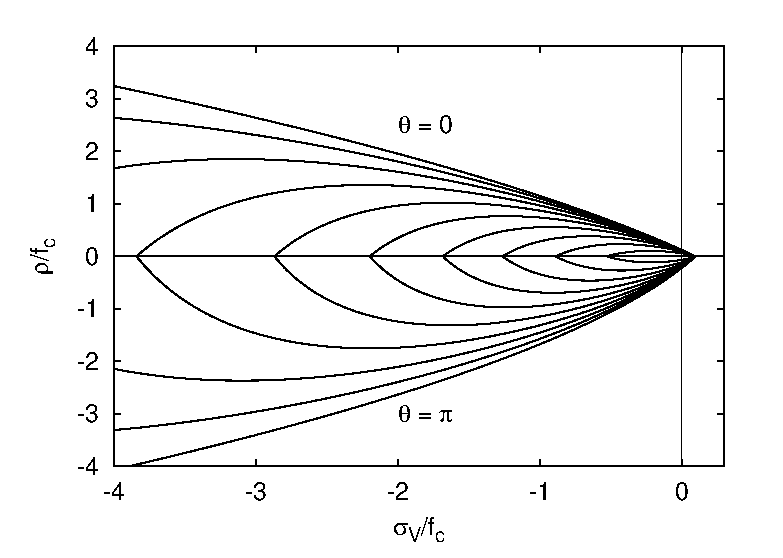
\includegraphics[width=0.5\textwidth]{meridians.eps}&
 % 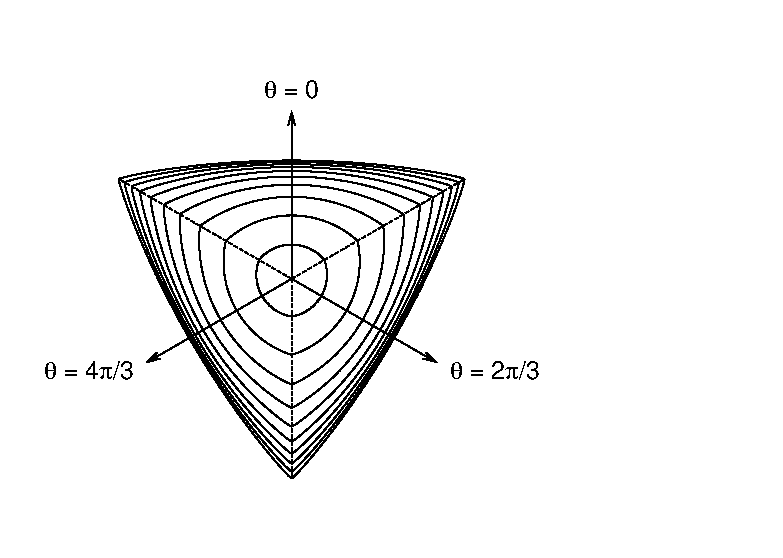
\includegraphics[width=0.5\textwidth]{deviatoric.eps}
%\end{htmlonly}
%begin{latexonly}
 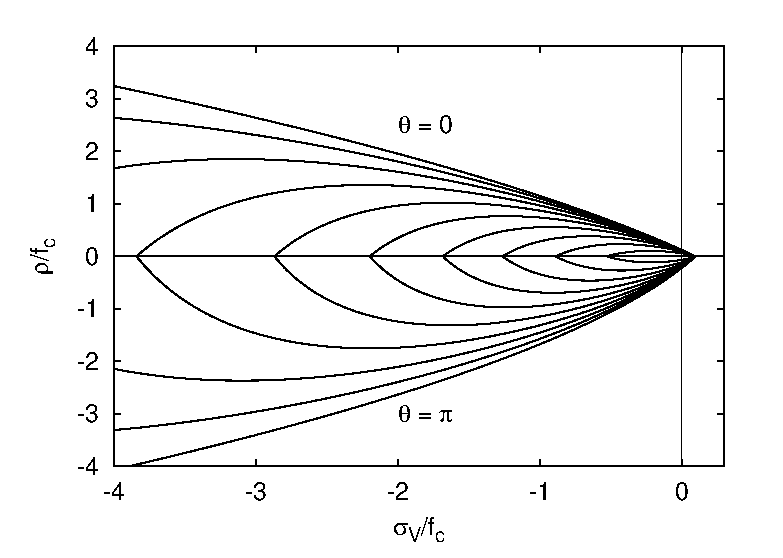
\includegraphics[width=0.5\textwidth]{meridians}&
 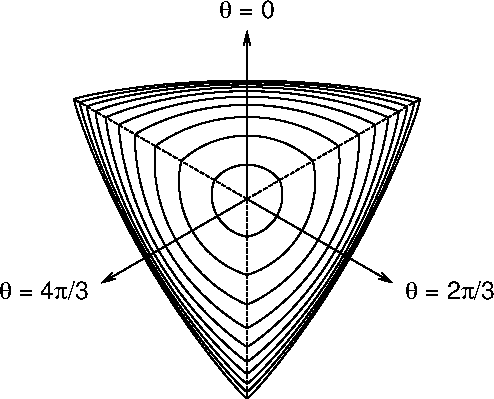
\includegraphics[width=0.5\textwidth]{deviatoric}
%end{latexonly}
\end{tabular} 
\caption{Evolution of the yield surface during hardening:
a) meridional section, b) deviatoric section for a constant volumetric effective stress of $\bar{\sigma}_{\rm V} = -\fc/3$} 
\label{fig:surfaceMerDev}
\end{figure}

The maximum size of the elastic domain is attained when the variable $q_{\rm h}$ is equal to one (which is its maximum value, as follows from the hardening law, to be specified in~(\ref{eq:hardeningLaw})). The yield surface is then described by the equation
%
\begin{equation}\label{eq:failureSurface}
f_{\rm p}\left(\bar{\sigma}_{\rm V},\bar{\rho},\bar{\theta};1\right) \equiv \frac{3}{2} \frac{\bar{\rho}^2}{\fc^2} + m_0 \left(\frac{\bar{\rho} }{\sqrt{6}\fc}r(\bar{\theta}) + \frac{\bar{\sigma}_{\rm V}}{\fc} \right) - 1 = 0
\end{equation}

The {\bf flow rule} 
%
\begin{equation} \label{eq:flowRuleDPM}
\dot{\mbf{\eps}}_{\rm p} = \dot{\lambda} \frac{\partial g_{\rm p}}{\partial\bar{\sigma}} 
\end{equation}
%
is non-associated, which means that the yield function $f_{\rm p}$ and the plastic potential 
\bea\nonumber
g_{\rm p}(\bar{\sigma}_{\rm V},\bar{\rho};\kappa_{\rm p})&=&\left(\left[1-q_{\rm{h}}(\kappa_{\rm p})\right] \left( \frac{\bar{\rho}} {\sqrt{6}\fc} + \frac{\bar{\sigma}_{\rm V}}{\fc} \right)^2 + \sqrt{\frac{3}{2}} \frac {\bar{\rho}}{\fc} \right)^2 +\\
&&+q_{\rm{h}}^2(\kappa_{\rm p}) \left( \frac{m_0 \bar{\rho}}{\sqrt{6}\fc} + \frac{m_{\rm g}(\bar{\sigma}_{\rm V})}{\fc} \right)
 \label{eq:plasticPotential}
\eea
do not coincide and, therefore, the direction of the plastic flow $\partial g_{\rm p}/\partial\bar{\vsig}$ is not normal to the yield surface.
The ratio of the volumetric and the deviatoric parts of the flow direction is controled by function $m_{\rm g}$, which depends on the volumetric stress and is defined as 
\begin{equation} \label{eq:mg}
m_{\rm g}(\bar{\sigma}_{\rm V})=A_{\rm g}B_{\rm g}\fc \exp{\frac{\bar{\sigma}_{\rm V} -\ft/3}{B_{\rm g}\fc}}
\end{equation}
%
where $A_{\rm g}$ and $B_{\rm g}$ are model parameters that are determined from certain assumptions on the plastic flow in uniaxial tension and compression.

The dimensionless variable $q_{\rm h}$ that appears in the yield function (\ref{eq:yieldSurface}) is a function of the hardening variable $\kappa_{\rm p}$. It controls the size and shape of the yield surface and, thereby, of the elastic domain. 
The {\bf hardening law} is given by
%
\begin{equation} \label{eq:hardeningLaw}
\qh(\kappa_{\rm p}) = \left\{ \begin{array}{ll}
{\qh}_0 + (1-{\qh}_0)\kappa_{\rm p}({\kappa_{\rm p}}^2 - 3\kappa_{\rm p}+3) & \mbox{if $\kappa_{\rm p} < 1$} \\
1 & \mbox{if $\kappa_{\rm p} \ge 1$}
\end{array}
\right.
\end{equation}
%
The initial inclination of the hardening curve (at $\kappa_{\rm p}=0$) is positive and finite, and the inclination at peak (i.e., at $\kappa_{\rm p} = 1$) is zero.


The evolution law for the hardening variable,\footnote{In the original paper \cite{GraJir},
equation (\ref{eq:dotkappap}) was written with $\cos^2\bar{\theta}$ instead of $(2\cos\bar{\theta})^2$,
but all the results presented in that paper were computed with OOFEM using an implementation based on (\ref{eq:dotkappap}).}
\begin{equation}\label{eq:dotkappap}
\dot{\kappa}_{\rm {p}} = \frac {\| \dot{\veps}_{\rm{p}}\|}{x_{\rm{h}}\left(\bar{\sigma}_{\rm V} \right)}(2\cos\bar{\theta})^2 
\end{equation}
sets the rate of the hardening variable equal to the norm of the plastic strain rate 
scaled by a hardening ductility measure 
\begin{equation} \label{eq:hardeningMeasure}
x_{\rm{h}}\left(\bar{\sigma}_{\rm V}\right) = \left\{ \begin{array}{ll}
A_{\rm{h}} - \left(A_{\rm{h}} - B_{\rm{h}} \right)\exp{\left(-R_{\rm h}(\bar{\sigma}_{\rm V})/C_{\rm h}\right)} & \mbox{if $R_{\rm h}(\bar{\sigma}_{\rm V}) \geq 0 $} \\[5mm]
E_{\rm h}\exp({R_{\rm h}(\bar{\sigma}_{\rm V})/F_{\rm h}})+D_{\rm h} & \mbox{if $R_{\rm h}(\bar{\sigma}_{\rm V}) < 0$}
\end{array}
\right.
\end{equation}
The dependence of the scaling factor
$x_{\rm{h}}$ on the volumetric effective stress $\bar{\sigma}_{\rm V}$ is constructed such that
the model response is more ductile under compression.
%
The variable 
\begin{equation}
R_{\rm h}(\bar{\sigma}_{\rm V}) = -\frac{\bar{\sigma}_{\rm V}}{\fc}-\frac{1}{3}
\end{equation}
is a linear function of the volumetric effective stress.
%
Model parameters $A_{\rm h}, B_{\rm h}, C_{\rm h}$ and $D_{\rm h}$ are calibrated from the values of strain at peak stress under uniaxial tension, uniaxial compression and triaxial compression, whereas the parameters 
\begin{eqnarray}
E_{\rm h} &=& B_{\rm h} - D_{\rm h}
\\
F_{\rm h} &=& \frac{\left(B_{\rm h} -D_{\rm h}\right)C_{\rm h}}{B_{\rm h} - A_{\rm h}}
\end{eqnarray}
are determined from the conditions of a smooth transition between the two parts of equation (\ref{eq:hardeningMeasure}) at $R_{\rm h} = 0$.

For the present model, the {\bf evolution of damage} starts after full saturation of plastic hardening, i.e., at $\kappa_{\rm p}=1$. This greatly facilitates calibration of model parameters, because the strength envelope is fully controled by the plastic part of the model and damage affects only the softening behavior.
In contrast to pure damage models,
damage is assumed to be driven by the plastic strain, more
specifically by its volumetric part, which is closely related 
to cracking. To slow down the evolution of damage under compressive stress states,
the damage-driving variable $\kappa_{\rm d}$ is not set equal to the volumetric
plastic strain, but it is defined incrementally by the rate equation
%
\begin{equation}\label{eq:equivStrain}
\dot{\kappa}_{\rm d} = \left\{ \begin{array}{ll}
0 & \mbox{if $\kappa_{\rm p}< 1$} \\
{\rm Tr}(\dot{\veps}_{\rm p})/x_{\rm s}\left(\bar{\sigma}_{\rm V}\right) & \mbox{if $\kappa_{\rm p}\ge 1$}
\end{array}
 \right.
\end{equation}
where
\begin{equation}\label{eq:damageDuctility}
x_{\rm s}(\bar{\sigma}_{\rm V}) = \left\{\begin{array}{ll}
1 + A_{\rm s}R_{\rm s}^2(\bar{\sigma}_{\rm V}) & \mbox{if $R_{\rm s}(\bar{\sigma}_{\rm V}) < 1$}\\[5mm]
1 - 3 A_{\rm s} + 4 A_{\rm s} \sqrt{R_{\rm s}(\bar{\sigma}_{\rm V})} & \mbox{if $R_{\rm s}(\bar{\sigma}_{\rm V}) \geq 1$}
\end{array}
\right .
\end{equation}
is a softening ductility measure.
Parameter $A_{\rm s}$ is determined from the softening response in uniaxial compression. The dimensionless variable
$R_{\rm s}=\dot{\varepsilon}_{\rm pV}^{-}/\dot{\varepsilon}_{\rm {pV}}$ is defined as the ratio between the ``negative'' volumetric plastic strain rate
%
\begin{equation}\label{eq:xs}
\dot{\varepsilon}_{\rm pV}^{-} = \displaystyle{\sum_{I = 1}^3 \langle-\dot{\varepsilon}_{\rm{p}I}\rangle}
\end{equation}
%
and the total volumetric plastic strain rate $\dot{\varepsilon}_{\rm {pV}}$.
This ratio depends only on the flow direction $\partial g_{\rm p}/\partial\bar{\vsig}$, and thus
$R_{\rm s}$ can be shown to be a unique function of the volumetric effective stress. In (\ref{eq:xs}), $\dot{\varepsilon}_{\rm{p}I}$ are the principal components of the rate of plastic strains and $\left<\cdot\right>$ denotes the McAuley brackets (positive-part operator).
For uniaxial tension, for instance, all three principal plastic strain rates are nonnegative, and so $\dot{\varepsilon}_{\rm pV}^{-} =0$, $R_{\rm s}=0$ and $x_{\rm s}=1$. This means that under uniaxial tensile loading we have $\kappa_{\rm d}=\kappa_{\rm p}-1$. On the other hand, under compressive stress states the negative principal plastic strain rates lead to a ductility measure $x_{\rm s}$ greater than one and the evolution of damage is slowed down. It should be emphasized that the flow rule for this specific model is constructed such that the volumetric part of plastic strain rate at the ultimate yield surface cannot be negative.

\begin{table}[!htb]
%\begin{center}
\begin{tabular}{|l|p{9cm}|}
\hline
Description & Damage-plastic model for concrete\\
\hline
Record Format & \descitem{ConcreteDPM}  \elemparam{d}{rn}
\elemparam{E}{rn} \elemparam{n}{rn} \elemparam{tAlpha}{rn}
 \elemparam{ft}{rn} \elemparam{fc}{rn} \elemparam{wf}{rn} \elemparam{Gf}{rn} \elemparam{ecc}{rn}
 \elemparam{kinit}{rn} \elemparam{Ahard}{rn} \elemparam{Bhard}{rn} \elemparam{Chard}{rn} \elemparam{Dhard}{rn} \elemparam{Asoft}{rn} \elemparam{helem}{rn} \elemparam{href}{rn} \elemparam{dilation}{rn} \elemparam{yieldtol}{rn} \elemparam{newtoniter}{in} \\
Parameters &- \param{d} material density\\
&- \param{E} Young modulus\\
&- \param{n} Poisson ratio\\
&- \param{tAlpha} thermal dilatation coefficient\\
&- \param{ft} uniaxial tensile strength $f_t$\\
&- \param{fc} uniaxial compressive strength\\
&- \param{wf} parameter $w_f$ that controls the slope of the softening branch (serves for the evaluation of $\eps_f=w_f/h$ to be used in (\ref{eq:damageLaw}))\\
&- \param{Gf} fracture energy, can be specified instead of wf, it is converted to $w_f=G_f/f_t$ \\
&- \param{ecc} eccentricity parameter $e$ from (\ref{bf103}), optional, default value 0.525\\
&- \param{kinit} parameter ${\qh}_0$ from (\ref{eq:hardeningLaw}), optional, default value 0.1\\
&- \param{Ahard} parameter $A_{\rm h}$ from (\ref{eq:hardeningMeasure}), optional, default value 0.08\\
&- \param{Bhard} parameter $B_{\rm h}$ from (\ref{eq:hardeningMeasure}), optional, default value 0.003\\
&- \param{Chard} parameter $C_{\rm h}$ from (\ref{eq:hardeningMeasure}), optional, default value 2\\
&- \param{Dhard} parameter $D_{\rm h}$ from (\ref{eq:hardeningMeasure}), optional, default value $10^{-6}$\\
&- \param{Asoft} parameter $A_{\rm s}$ from (\ref{eq:damageDuctility}), optional, default value 15\\
&- \param{helem} element size $h$, optional (if not specified, the actual element size is used)\\
&- \param{href} reference element size $h_{ref}$, optional (if not specified, the standard adjustment of the damage law is used)\\
&- \param{dilation} dilation factor (ratio between lateral and axial plastic strain rates in the softening regime under uniaxial compression), optional, default value -0.85\\
&- \param{yieldtol} tolerance for the implicit stress return algorithm, optional, default value $10^{-10}$\\
&- \param{newtoniter} maximum number of iterations in the implicit stress return algorithm, optional, default value 100\\
Supported modes& 3dMat\\
\hline
\end{tabular}
\caption{Damage-plastic model for concrete -- summary.}
\label{dpm_table}
%\end{center}
\end{table}


The relation between the damage variable $\omega$ and the internal variable $\kappa_{\rm d}$ (maximum level of equivalent strain) is assumed to have the exponential form 
\begin{equation} \label{eq:damageLaw}
\omega = 
1-\exp\left(-\kappa_{\rm d}/\varepsilon_f\right) 
\end{equation}
where $\varepsilon_f$ is a parameter that controls the slope of the softening curve. In fact, equation (\ref{eq:damageLaw}) is used by the nonlocal version
of the damage-plastic model, with $\kappa_{\rm d}$ replaced by its weighted
spatial average (not yet available in the public version of OOFEM).
For the local model, it is necessary to adjust softening according
to the element size, otherwise the results would suffer by pathological 
mesh sensitivity. It is assumed that localization takes place at the
peak of the stress-strain diagram, i.e., at the onset of damage. 
After that, the strain is decomposed into the distributed
part, which corresponds to unloading from peak, and the localized part,
which is added if the material is softening.
The  localized part of strain 
is transformed into an equivalent crack opening, $w$, which is 
under uniaxial tension linked
to the stress by the exponential law 
\begin{equation} \label{eq:damageLaw2}
\sigma = (1-\omega) f_t =
f_t \exp\left(-w/w_f\right) 
\end{equation}
Here, $f_t$ is the uniaxial tensile strength and $w_f$ is the characteristic
crack opening, playing a similar role to $\varepsilon_f$.
Under uniaxial tension, the localized strain can be expressed as the sum
of the post-peak plastic strain (equal to variable $\kappa_{\rm d}$) 
and the unloaded part of elastic strain (equal to $\omega f_t/E$).
Denoting the effective element size as $h$, we can write
\begin{equation}
w = h(\kappa_{\rm d}+\omega f_t/E)
\end{equation}
and substituting this into (\ref{eq:damageLaw2}), we obtain a nonlinear
equation
\begin{equation}\label{eq:damageLaw4}
1-\omega = \exp\left(-\frac{h}{w_f}\left(\kappa_{\rm d}+\omega f_t/E\right)\right)
\end{equation}
from which the damage variable $\omega$ corresponding to the given internal
variable $\kappa_{\rm d}$ can be computed by Newton iteration.
The effective element size $h$ is obtained by projecting the element onto
the direction of the maximum principal strain at the onset of cracking,
and afterwards it is held fixed. The evaluation of $\omega$ from
$\kappa_{\rm d}$ is no longer explicit, but the resulting load-displacement curve
of a bar under uniaxial tension is totally independent of the mesh size.
A simpler approach would be to use (\ref{eq:damageLaw}) with 
$\varepsilon_f = w_f/h$, but then the scaling would not be perfect and
the shape of the load-displacement curve (and also the dissipated energy)
would slightly depend on the mesh size. With the present approach,
the energy per unit sectional area dissipated under uniaxial tension 
is exactly $G_f = w_f f_t$. The input parameter controling the damage law
can be either the characteristic crack opening $w_f$, 
or the fracture energy $G_f$. If both are specified, $w_f$ is used and
$G_f$ is ignored. If only $G_f$ is specified, $w_f$ is set to $G_f/f_t$.

The onset of damage corresponds to the peak of the stress-strain diagram
under proportional loading, when the ratios of the stress components are fixed.
This is the case e.g.\ for uniaxial tension, uniaxial compression, or shear
under free expansion of the material (with zero normal stresses). However,
for shear under confinement the shear stress can rise even after the onset
of damage, due to increasing hydrostatic pressure, which increases the
mobilized friction. It has been observed that the standard approach leads
to strong sensitivity of the peak shear stress to the element size.
To reduce this pathological effect, a modified approach has been implemented.
The second-order work (product of stress increment and strain increment)
is checked after each step and the element-size dependent adjustment
of the damage law is applied only after the second-order work becomes negative.
Up to this stage, the damage law corresponds to a fixed reference element
size, which is independent of the actual size of the element.
This size is set by the optional parameter \param{href}.
If this parameter is not specified, the standard approach is used.
For testing purposes, one can also specify the actual element size,
\param{helem}, as a ``material property''. If this parameter is not
specified, the element size is computed for each element separately
and represents its actual size.  

The damage-plastic model contains 15 parameters, but only 6 of them need to be actually calibrated for different concrete types, namely Young's modulus $E$, Poisson's ratio $\nu$, tensile strength $f_{\rm t}$, compressive strength $f_{\rm c}$, parameter $w_f$ (or fracture energy $G_f$), and parameter $A_{\rm s}$ in the ductility measure (\ref{eq:damageDuctility}) of the damage model. The remaining parameters can be set to their default values specified in \cite{GraJir}.

The model parameters are summarized
in Tab.~\ref{dpm_table}. Note that it is possible to specify the ``size'' of finite element, $h$, which (if specified) replaces
the actual element size in  (\ref{eq:damageLaw4}). The usual approach is to consider $h$ as the actual element size (evaluated automatically by OOFEM), 
in which case the optional
parameter $h$ is missing (or is set to 0., which has the same effect in the code). However, for various studies of mesh sensitivity
it is useful to have the option of  specifying $h$ as an input ``material'' value.

If the element is too large, it may become too brittle and local snap-back
occurs in the stress-strain diagram, which is not acceptable. 
In such a case, an error message is issued and the program execution
is terminated. The maximum admissible element size 
\begin{equation}
h_{\max} = \frac{EG_f}{f_t^2} = \frac{Ew_f}{f_t}
\end{equation}
happens to be equal to Hillerborg's characteristic material length. 
For typical concretes it is in the order of a few hundred mm. 
If the condition $h<h_{\max}$ is violated, the mesh needs to be refined.
Note that the effective element size $h$ is obtained by projecting the element.
For instance, if the element is a cube of edge length 100 mm, its effective
size in the direction of the body diagonal can be 173 mm. 

\subsection{Orthotropic damage model with fixed crack orientations for composites - CompDamMat}

The model is designed for transversely isotropic elastic material defined by five elastic material constants. Typical example is a carbon fiber tow. Axis $1$ represents the material principal direction. The orthotropic material constants are defined as
\begin{eqnarray}
\nu_{12}&=&\nu_{13},~\nu_{21}=\nu_{31},~\nu_{23}=\nu_{32},~E_{22}=E_{33}\\
G_{12}&=&G_{13}=G_{21}=G_{31},G_{23}=G_{32}\\
\frac{\nu_{12}=\nu_{13}}{E_{11}} &=& \frac{\nu_{21}=\nu_{31}}{E_{22}},~\frac{\nu_{31}=\nu_{21}}{E_{33}} = \frac{\nu_{13}=\nu_{12}}{E_{11}}
\end{eqnarray}

Material orientation on a finite element can be specified with \param{lcs} optional parameter. If unspecified, material orientation is the same as the global coordinate system. \param{lcs} array contains six numbers,
where the first three numbers represent a directional vector of the local $x$-axis, and the next three numbers represent a directional vector of the local $y$-axis with the reference to the global coordinate system. The composite material is extended to 1D and is also suitable for beams and trusses. In such particular case, the \param{lcs} has no effect and the 1D element orientation is aligned with the global $xx$ component.

The index $p,~p\in\{11,22,33,23,31,12\}$ symbolizes six components of stress or strain vectors. The linear softening occurs after reaching a critical stress $f_{p,0}$, see Fig. \ref{comp_softening}. Orientation of cracks is assumed to be orthogonal and aligned with an orientation of material axes \cite[pp.236]{Bazant:98}. The transverse isotropy is generally lost upon fracture, material becomes orthotropic and six damage parameters $d_p$ are introduced.

\begin{figure}[!htb]
\begin{htmlonly}
  \centerline{\includegraphics[width=0.7\textwidth]{Compodamagemat_diag.eps}}
\end{htmlonly}
%begin{latexonly}
 \centerline{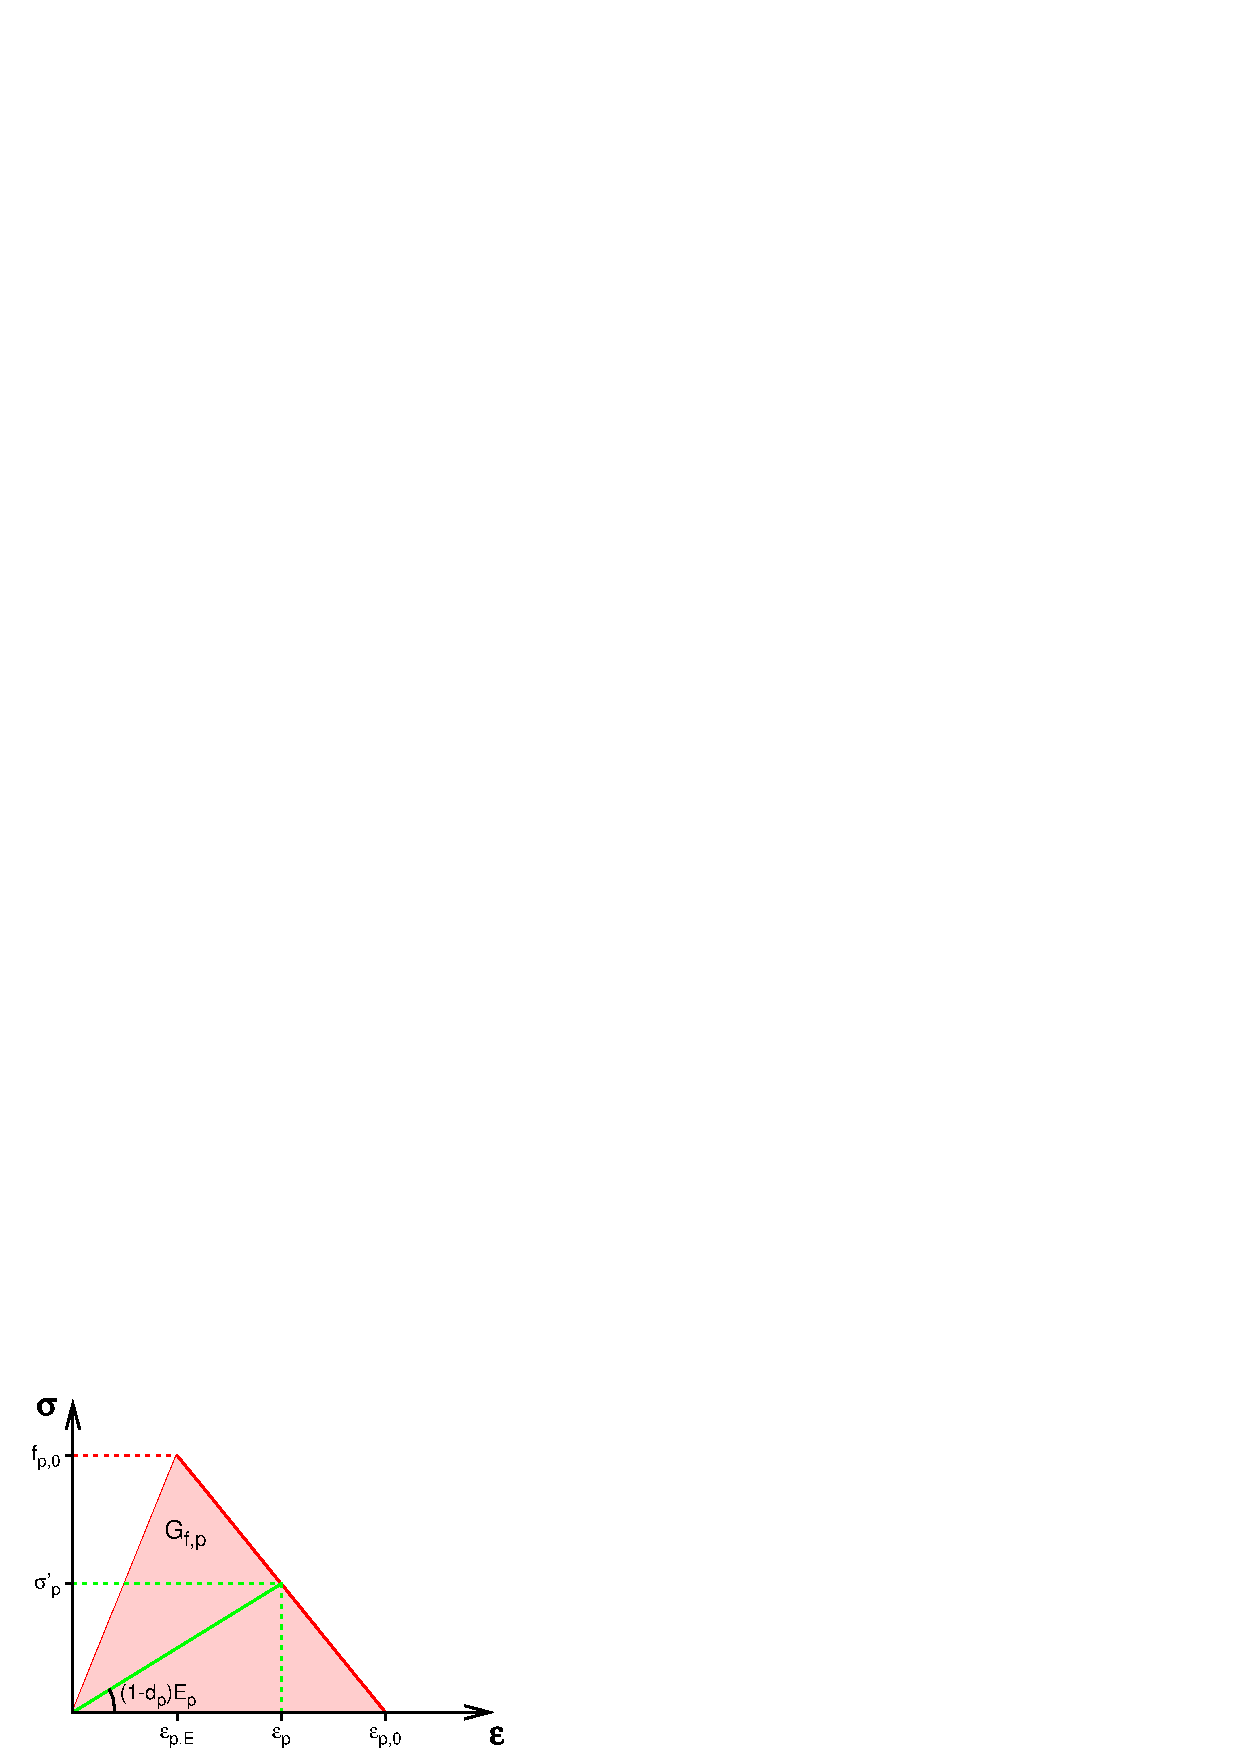
\includegraphics[width=0.7\textwidth]{Compodamagemat_diag}}
%end{latexonly}
  \caption{Implemented stress-strain evolution with damage for 1D case. Tension and compression are separated, but sharing the same damage parameter.}
  \label{comp_softening}
\end{figure}

The compliance material matrix $\mathbf{H}$, in the secant form and including damage parameters, reads
\footnotesize
\begin{equation}
\mathbf{H}=
\left[ \begin{array}{cccccc}
\frac{1}{(1-d_{11})E_{11}} & -\frac{\nu_{21}}{E_{22}} & -\frac{\nu_{31}}{E_{33}} &0 &0 & 0\\
-\frac{\nu_{12}}{E_{11}} & \frac{1}{(1-d_{22})E_{22}} & -\frac{\nu_{32}}{E_{33}} &0& 0&0\\
-\frac{\nu_{13}}{E_{11}} & -\frac{\nu_{23}}{E_{22}} & \frac{1}{(1-d_{33})E_{33}} &0 &0 &0 \\
 0&0 &0 & \frac{1}{(1-d_{23})G_{23}} & 0&0 \\
 0& 0& 0& 0& \frac{1}{(1-d_{31})G_{31}} & 0\\
 0& 0&0 &0& 0& \frac{1}{(1-d_{12})G_{12}}
\end{array} \right]\label{comp_eq_H}
\end{equation}
\normalsize

Damage occurs when any out of six stress tensor components exceeds a given strength $f_{p,0}$
\begin{equation}
|\sigma_p| \geq |f_{p,0}|
\end{equation}
Positive and negative ultimate strengths can be generally different but share the same damage variable.
At the point of damage initiation, see Fig. \ref{comp_softening}, one evaluates $\varepsilon_{p,E}$ and characteristic element length $l_p$, generally different for each damage mode. Given the fracture energy $G_{F,p}$, the maximum strain at zero stress $\varepsilon_{p,0}$ is computed
\begin{eqnarray}
\varepsilon_{p,0} &=& \varepsilon_{p,E} + \frac{2G_{F,p}}{f_{p,0} l_p}
\end{eqnarray}

The point of damage initiation is never reached exactly, one needs to interpolate between the previous equilibrated step and current step to achieve objectivity.

The evolution of damage $d_p$ is based on the evolution of corresponding strain $\varepsilon_p$. A maximum achieved strain is stored in the variable $\kappa_p$. If $\varepsilon_p > \kappa_p$ the damage may grow so the corresponding damage variable $d_p$ may increase. Desired stress $\sigma'_p$ is evaluated from the actual strain $\varepsilon_p$
\begin{eqnarray}
\sigma'_p &=& f_{p,0} \frac{\varepsilon_{p,0} - \varepsilon_p}{\varepsilon_{p,0}-\varepsilon_{p,E}}
\end{eqnarray}
and the calculation of damage variables $d_p$ stems from Eq.~\ref{comp_eq_H}, for example
\begin{eqnarray}
d_{11} &=& 1 - \frac{\sigma'_{11}}{E_{11}\left(\varepsilon_{11}+\frac{\nu_{21}}{E_{22}}\sigma_{22}+ \frac{\nu_{31}}{E_{33}}\sigma_{33} \right)}\\
d_{12} &=& 1 - \frac{\sigma'_{12}}{G_{12}\varepsilon_{12}}
\end{eqnarray}
Damage is always controled not to decrease. Fig.~\ref{comp_performance} shows a typical performance for this damage model in one direction.

The damage initiation is based on a trial stress. It becomes necessary for  higher precision to skip a few first iteration, typically 5, and then to introduce damage. A parameter \param{afterIter} is designed for this purpose and \param{MinIter} forces a solver always to proceed certain amount of iterations.

\param{allowSnapBack} skips the checking of sufficient fracture energy for each direction. If not specified, all directions are checked to prevent snap-back which dissipates incorrect amount of energy.


\begin{figure}[!htb]
\begin{htmlonly}
  \centerline{\includegraphics[width=0.7\textwidth]{Compodamagemat_test.eps}}
\end{htmlonly}
%begin{latexonly}
\centerline{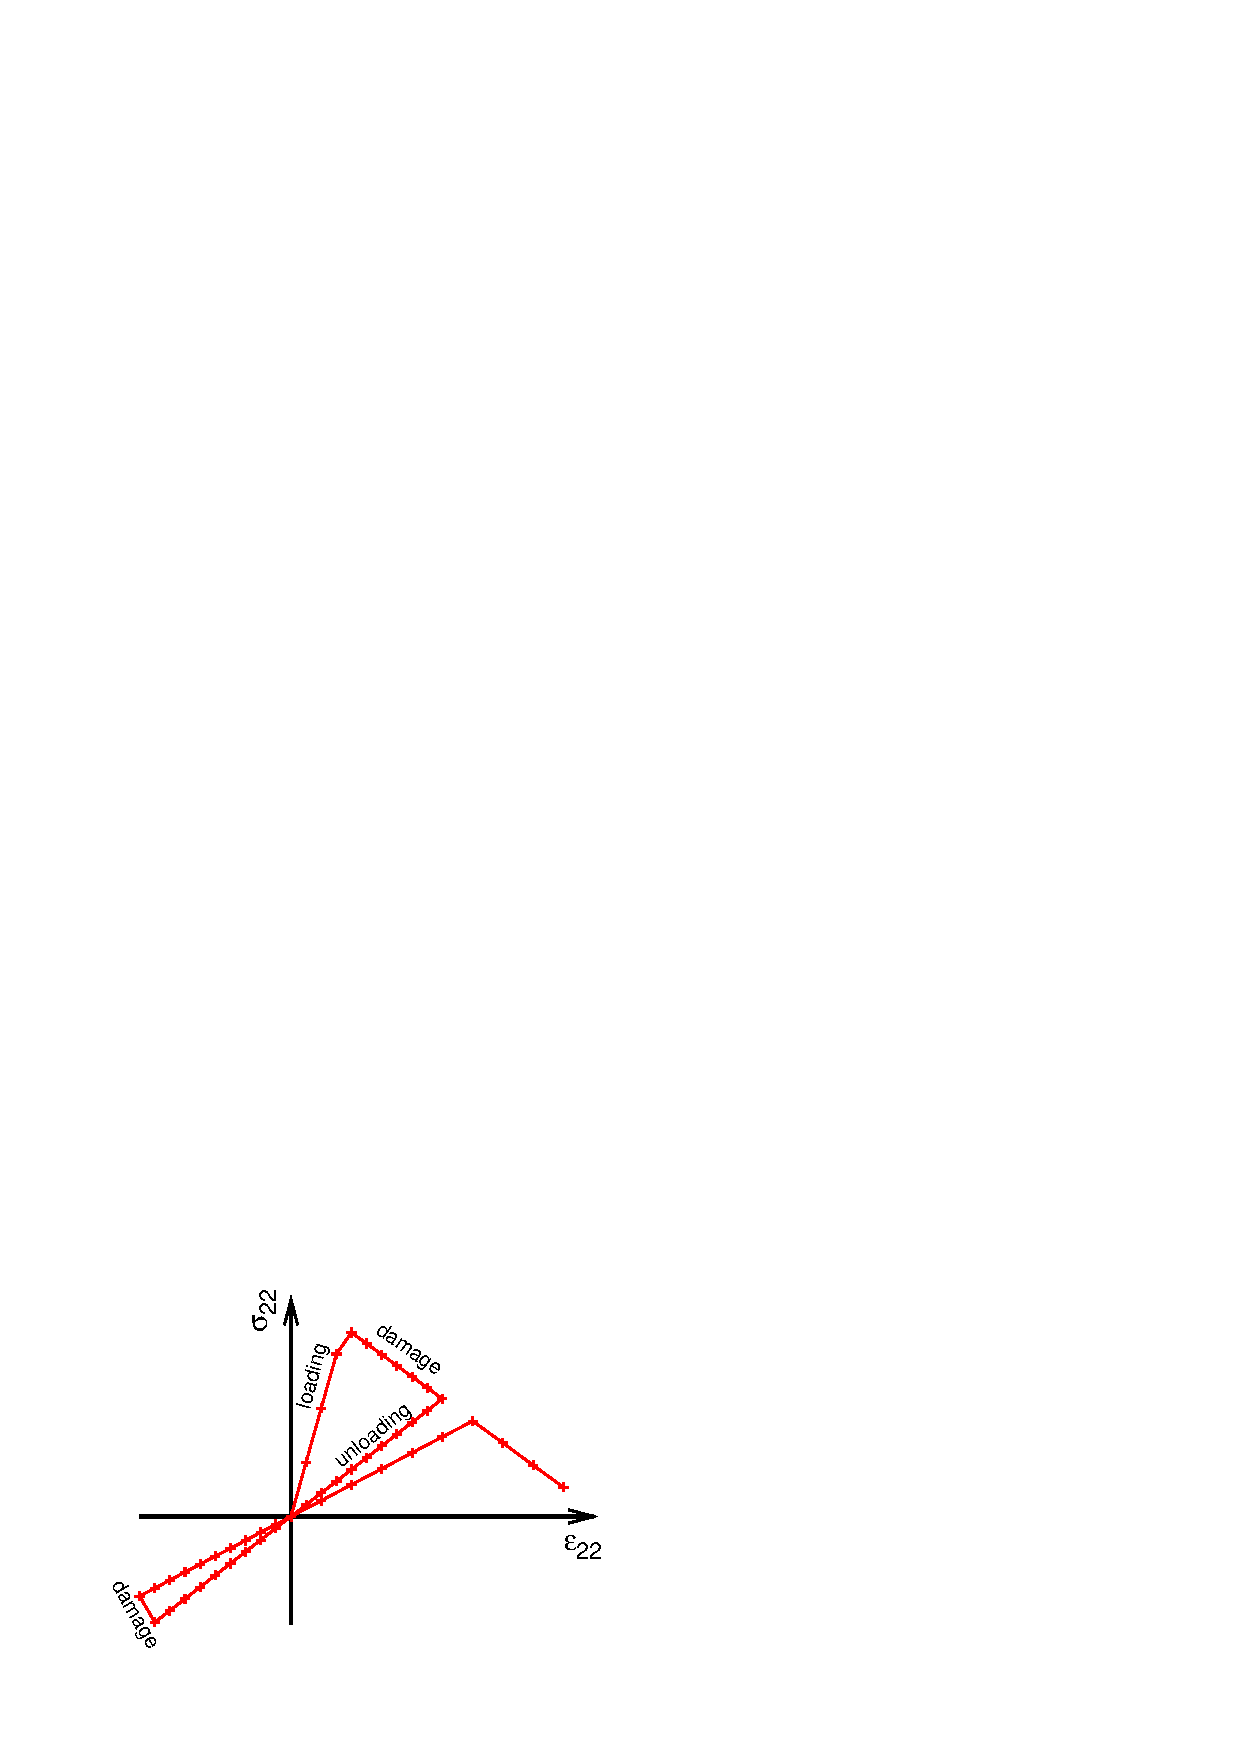
\includegraphics[width=0.7\textwidth]{Compodamagemat_test}}
%end{latexonly}
  \caption{Typical loading/unloading material performance for homogenized stress and strain in the direction `${2}$'. Note that one damage parameter is common for both tension and compression.}
  \label{comp_performance}
\end{figure}

\begin{table}[!htb]
\begin{tabular}{|l|p{9cm}|}
\hline
Description & Orthotropic damage model with fixed crack orientations for composites\\
\hline
Record Format & \descitem{CompDamMat}  \elemparam{num}{in}
\elemparam{d}{rn} \elemparam{Exx}{rn} \elemparam{EyyEzz}{rn}
\elemparam{nuxynuxz}{rn} \elemparam{nuyz}{rn} \elemparam{GxyGxz}{rn}
\elemparam{Tension\_f0\_Gf}{ra} \elemparam{Compres\_f0\_Gf}{ra} [\elemparam{afterIter}{in}] [\elemparam{allowSnapBack}(ia)]\\
Parameters
&- \param{num} material model number\\
&- \param{d} material density\\
&- \param{Exx} Young's modulus for principal direction $xx$\\
&- \param{EyyEzz} Young's modulus in orthogonal directions to the principal direction $xx$\\
&- \param{nuxynuxz} Poisson's ratio in $xy$ and $xz$ directions\\
&- \param{nuyz} Poisson's ratio in $yz$ direction\\
&- \param{GxyGxz} shear modulus in $xy$ and $xz$ directions\\
&- \param{Tension\_f0\_Gf} array with six pairs of positive numbers. Each pair describes maximum stress in tension and fracture energy for each direction ($xx$, $yy$, $zz$, $yz$, $zx$, $xy$)\\
&- \param{Compres\_f0\_Gf} array with six pairs of numbers. Each pair describes maximum stress in compression (given as a negative number) and positive fracture energy for each direction ($xx$, $yy$, $zz$, $yz$, $zx$, $xy$)\\
Supported modes& 3dMat, 1dMat\\
&- \param {afterIter} how many iterations must pass until damage is computed from strains, zero is default. User must ensure that the solver proceeds the minimum number of iterations.\\
&- \param {allowSnapBack} array to skip checking for snap-back. The array members are 1-6 for tension and 7-12 for compression components.\\
\hline
\end{tabular}
\caption{Orthotropic damage model with fixed crack orientations for composites -- summary.}
\label{compdammat_table}
\end{table}



\subsection{Orthotropic elastoplastic model with isotropic damage - TrabBone3d}

This model combines orthotropic elastoplasticity with isotropic damage.
Material orthotropy is described by the fabric tensor, i.e., a symmetric second-order
tensor with principal directions aligned with the axes of orthotropy and principal
values normalized such that their sum is 3. Elastic constants as well as coefficients
that appear in the yield condition are linked to the principal values of the
fabric tensor and to porosity. The yield condition is piecewise quadratic,
with different parameters in the regions of positive and negative volumetric strain. 

\subsubsection{Local formulation}
The basic equations include an additive decomposition of total strain into elastic (reversible) part and plastic (irreversible) part
\begin{equation}\label{additiveDecomposition}
\veps = \veps_{\rm{e}}+\veps_{\rm{p}},
\end{equation}
the stress strain law
\begin{equation}\label{constitutiveLaw}
\vsig = \left(1-\omega\right)\bar{\vsig}=\left(1-\omega\right)\mbf{D}:{\veps}_{\rm{e}},
\end{equation}
the yield function 
\begin{equation}
f(\bar{\vsig},\kappa) = \sqrt{\bar{\vsig} :\mbf{F}:\bar{\vsig}} - \sigma_Y(\kappa).
\end{equation}
loading-unloading conditions
\begin{equation}
f(\bar{\vsig},\kappa)\le 0 \qquad \dot{\lambda}\geq 0 \qquad \dot{\lambda}f(\bar{\vsig},\kappa)=0,
\end{equation}
evolution law for plastic strain
\begin{equation}
\dot{\veps}_{\rm{p}} = \dot{\lambda} \frac{\partial f}{\partial \bar{\vsig}},
\end{equation}
the incremental definition of cumulated plastic strain
\begin{equation}
\dot{\kappa} = \| \epspd \|,
\end{equation}
the law governing the evolution of the damage variable
\begin{equation}
\omega(\kappa) = \omega_c(1-\mbox{e}^{-a\kappa}),
\end{equation}
and the hardening law
\begin{equation}
\sigma_Y(\kappa) = 1+\sigma_H(1-\mbox{e}^{-s\kappa}).
\end{equation}
In the equations above, $\bar{\vsig}$~is the effective stress tensor, $\mbf{D}$~is the elastic stiffness tensor, $f$~is the yield function, $\lambda$ is the consistency parameter (plastic multiplier), $\omega$~is the damage variable, $\sigma_Y$~is the yield stress and $s$, $a$, $\sigma_H$ and  $\omega_c$~are positive material parameters. 
Material anisotropy is characterized by the second-order positive definite  fabric tensor 
\begin{equation}\label{fabric}
\mbf{M} = \sum_{i=1}^3 m_i(\mbf{m}_i \otimes \mbf{m}_i),
\end{equation}
normalized such that Tr$(\mbf{M}) = 3$, $m_i$ are the eigenvalues and $\mbf{m}_i$ the eigenvectors.
The eigenvectors of the fabric tensor determine the directions of material orthotropy and the components of the elastic stiffness tensor $\mbf{D}$ are linked to eigenvalues of the fabric tensor. In the coordinate system aligned with $m_i$, $i=1,2,3$,
the stiffness can be presented in Voigt (engineering) notation as
\begin{equation}
  \mbf{D}=\left[\begin{array}{cccccc}
\frac{1}{E_1} & -\frac{\nu_{12}}{E_1}&-\frac{\nu_{13}}{E_1}& 0& 0&0\\
-\frac{\nu_{21}}{E_2} & \frac{1}{E_2}&-\frac{\nu_{23}}{E_2}& 0& 0&0\\
-\frac{\nu_{31}}{E_3} & -\frac{\nu_{32}}{E_3}&\frac{1}{E_3}& 0& 0&0\\
0 & 0 & 0 & \frac{1}{G_{23}} & 0 & 0\\
0 & 0 & 0 & 0 & \frac{1}{G_{13}} & 0\\
0 & 0 & 0 & 0 & 0 & \frac{1}{G_{12}}
 \end{array}\right]^{-1},
\end{equation}
where $E_i = E_0\rho^k m_i^{2l}$, $G_{ij} = G_0 \rho^k m_i^l m_j^l$  and $\nu_{ij} = \nu_0 \frac{m_i^l}{m_j^l}$. Here, $E_0$, $G_0$ and $\nu_0$ are elastic constants characterizing the compact (poreless) material, $\rho$ is the volume fraction of solid phase and $k$ and $l$ are dimensionless exponents.

Similar relations as for the stiffness tensor are also postulated for the components of a fourth-order tensor $\mbf{F}$ that is used in the yield condition. The yield condition is divided into tensile and compressive parts. Tensor $\mbf{F}$ is different in each part of the effective stress space. This tensor is denoted $\mbf{F}^{+}$ in tensile part, characterized by $\hat{\mbf{N}}:\bar{\vsig} \leq 0$ and $\mbf{F}^{-}$ in compressive part, characterized by $\hat{\mbf{N}}:\bar{\vsig} \leq 0$, where
\begin{equation}
\hat{\mbf{N}} = \frac{\sum_{i=1}^{3} m_i^{-2q}}{\sqrt{\sum_{i=1}^3 m_i^{-4q}}}(\mbf{m}_i \otimes \mbf{m}_i)
\end{equation}

\begin{equation}
  \mbf{F^{\pm}}=\left[\begin{array}{cccccc}
\frac{1}{\left({\sigma_{1}^{\pm}}\right)^2} & -\frac{\chi_{12}^{\pm}}{\left({\sigma_{1}^{\pm}}\right)^2}&-\frac{\chi_{13}^{\pm}}{\left({\sigma_{1}^{\pm}}\right)^2}& 0& 0&0\\
-\frac{\chi_{21}^{\pm}}{\left({\sigma_{2}^{\pm}}\right)^2} & \frac{1}{\left({\sigma_{2}^{\pm}}\right)^2}&-\frac{\chi_{23}^{\pm}}{\left({\sigma_{2}^{\pm}}\right)^2}& 0& 0&0\\
-\frac{\chi_{31}^{\pm}}{\left({\sigma_{3}^{\pm}}\right)^2} & -\frac{\chi_{32}^{\pm}}{\left({\sigma_{3}^{\pm}}\right)^2}&\frac{1}{\left({\sigma_{3}^{\pm}}\right)^2}& 0& 0&0\\
0 & 0 & 0 & \frac{1}{\tau_{23}} & 0 & 0\\
0 & 0 & 0 & 0 & \frac{1}{\tau_{13}} & 0\\
0 & 0 & 0 & 0 & 0 & \frac{1}{\tau_{12}}
 \end{array}\right].
\end{equation}
In the equation above $\sigma_i^{\pm} = \sigma_0^{\pm}\rho^p m_i^{2q}$ is uniaxial yield stress along the $i$-th principal axis of orthotropy, $\tau_{ij} = \tau_0 \rho^p m_i^q m_j^q$ is the shear yield stress in the plane of orthotropy and $\chi_{ij}^{\pm} = \chi_0^{\pm}\frac{m_i^{2q}}{m_j^{2q}}$ is the so-called interaction coefficient, $p$ and $q$ are dimensionless exponents and parameters with subscript $0$ are related to a fictitious material with zero porosity. The yield surface is continuously differentiable if the parameters values are constrained by the condition
\begin{equation}
\frac{\chi_0^- +1}{(\sigma_0^-)^2} = \frac{\chi_0^+ +1}{(\sigma_0^+)^2}.
\end{equation}
The model description and parameters are summarized in Tab.~\ref{trabbone_table}.
\begin{table}[!htb]
%\begin{center}
\begin{tabular}{|l|p{9cm}|}
\hline
Description & Anisotropic elastoplastic model with isotropic damage\\
\hline
Record Format & \descitem{TrabBone3d}  \elemparam{}{in}
\elemparam{d}{rn} \elemparam{eps0}{rn} \elemparam{nu0}{rn} \elemparam{mu0}{rn} \elemparam{expk}{rn} \elemparam{expl}{rn} \elemparam{m1}{rn} \elemparam{m2}{rn} \elemparam{rho}{rn}
\elemparam{sig0pos}{rn} \elemparam{sig0neg}{rn} \elemparam{chi0pos}{rn} \elemparam{chi0neg}{rn} \elemparam{tau0}{rn} \elemparam{plashardfactor}{rn} \elemparam{expplashard}{rn} \elemparam{expdam}{rn} \elemparam{critdam}{rn}\\
Parameters &- \param{} material number\\
&- \param{d} material density\\
&- \param{eps0} Young modulus (at zero porosity)\\
&- \param{nu0} Poisson ratio (at zero porosity)\\
&- \param{mu0} shear modulus of elasticity (at zero porosity)\\
&- \param{m1} first eigenvalue of the fabric tensor\\
&- \param{m2} second eigenvalue of the fabric tensor\\
&- \param{rho} volume fraction of solid phase\\
&- \param{sig0pos} yield stress in tension\\
&- \param{sig0neg} yield stress in compression\\
&- \param{tau0} yield stress in shear\\
&- \param{chi0pos} interaction coefficient in tension\\
&- \param{plashardfactor} hardening parameter\\
&- \param{expplashard} exponent in hardening law\\
&- \param{expdam} exponent in damage law\\
&- \param{critdam} critical damage\\
&- \param{expk} exponent $k$ in the expression for elastic stiffness\\
&- \param{expl} exponent $l$ in the expression for elastic stiffness\\
&- \param{expq} exponent $q$ in the expression for tensor \mbf{F}\\
&- \param{expp} exponent $p$ in the expression for tensor \mbf{F}\\
Supported modes& 3dMat\\
\hline
\end{tabular}
\caption{Anisotropic elastoplastic model with isotropic damage - summary.}
\label{trabbone_table}
%\end{center}
\end{table}
\subsubsection{Nonlocal formulation - TrabBoneNL3d}
The model is regularized by the over-nonlocal formulation with damage driven by a combination of local and nonlocal cumulated plastic strain
\begin{equation}\label{overKappa}
\hat{\kappa} = (1-m)\kappa + m\bar{\kappa},
\end{equation}
where $m$ is a dimensionless material parameter (typically $m>1$) and
\begin{equation}\label{nonLocalPlStrain}
\bar{\kappa}(x) = \int\limits_V \alpha(x,s)\kappa(s)\,{\rm d}s
\end{equation}
is the nonlocal cumulated plastic strain. The nonlocal weight function is defined as
\begin{equation}
\alpha(x,s) = \frac{\alpha_0(\Vert x-s\Vert )}{\int\limits_V\alpha_0(\Vert x-t\Vert )\,{\rm d}t}
\end{equation}
where
\begin{equation}
\alpha_0(r) =\left\{\begin{array}{cc} \left(1-\frac{r^2}{R^2}\right)^2 & \mbox{ if } r\le R \\ 0 & \mbox{ if } r> R \end{array}\right.
\end{equation}
Parameter $R$ is related to the internal length of the material.
The model description and parameters are summarized in Tab.~\ref{trabboneNl_table}.
\begin{table}[!htb]
%\begin{center}
\begin{tabular}{|l|p{9cm}|}
\hline
Description & Nonlocal anisotropic elastoplastic model with isotropic damage\\
\hline
Record Format & \descitem{TrabBoneNL3d}  \elemparam{}{in}
\elemparam{d}{rn} \elemparam{eps0}{rn} \elemparam{nu0}{rn} \elemparam{mu0}{rn} \elemparam{expk}{rn} \elemparam{expl}{rn} \elemparam{m1}{rn} \elemparam{m2}{rn} \elemparam{rho}{rn}
\elemparam{sig0pos}{rn} \elemparam{sig0neg}{rn} \elemparam{chi0pos}{rn} \elemparam{chi0neg}{rn} \elemparam{tau0}{rn} \elemparam{plashardfactor}{rn} \elemparam{expplashard}{rn} \elemparam{expdam}{rn} \elemparam{critdam}{rn} \elemparam{m}{rn} \elemparam{R}{rn}\\
Parameters &- \param{} material number\\
&- \param{d} material density\\
&- \param{eps0} Young modulus (at zero porosity)\\
&- \param{nu0} Poisson ratio (at zero porosity)\\
&- \param{mu0} shear modulus (at zero porosity)\\
&- \param{m1} first eigenvalue of the fabric tensor\\
&- \param{m2} second eigenvalue of the fabric tensor\\
&- \param{rho} volume fraction of the solid phase\\
&- \param{sig0pos} yield stress in tension\\
&- \param{tau0} yield stress in shear\\
&- \param{chi0pos} interaction coefficient in tension\\
&- \param{chi0neg} interaction coefficient in compression\\
&- \param{plashardfactor} hardening parameter\\
&- \param{expplashard} exponent in the hardening law\\
&- \param{expdam} exponent in the damage law\\
&- \param{critdam} critical damage\\
&- \param{expk} exponent $k$ in the expression for elastic stiffness\\
&- \param{expl} exponent $l$ in the expression for elastic stiffness\\
&- \param{expq} exponent $q$ in the expression for tensor \mbf{F}\\
&- \param{expp} exponent $p$ in the expression for tensor \mbf{F}\\
&- \param{m} over-nonlocal parameter\\
&- \param{R} nonlocal interaction radius\\
Supported modes& 3dMat\\
\hline
\end{tabular}
\caption{Nonlocal formulation of anisotropic elastoplastic model with isotropic damage -- summary.}
\label{trabboneNl_table}
%\end{center}
\end{table}


\subsection{Material models for interfaces}

Interface elements have to be used with material models describing
the constitutive behavior of interfaces between two materials 
(e.g.\ between steel reinforcement and concrete),
or between two bodies in contact.
Such interface laws are formulated in terms of the traction vector and the displacement jump vector.

\subsubsection{Isotropic damage model for interfaces}

This model is described in Section~\ref{sec:idmfi}.

\subsubsection{Simple interface material}

This model provides a simple interface law with penalty-type contact and friction. 
In the normal direction, the response is linear elastic, but with different stiffnesses in tension and in compression (stiffness \param{kn} in compression, \param{kn}*\param{stiffcoeff} in tension). 
By setting \param{kn} to a high value, the penetration (overlap) can be reduced,
in the sense of the penalty approach. By setting  \param{stiffcoeff} to 0, free opening
of the gap can be allowed.
The shear response is elastoplastic, with the yield limit dependent on the normal traction. Crosssection's width, height or area have no influence on the results.
The magnitude of the shear traction $\vsig_T$ must not exceed the yield limit computed 
according to a Coulomb-like friction law as the product of the (negative part of)
 normal traction $\sigma_N$ and a dimensionless coefficient of friction $fc$:
\begin{equation}
    ||\vsig_T|| \leq \left\langle-\sigma_N\cdot fc\right\rangle 
\end{equation}
$\sigma_N$ is computed multiplying a known normal strain and a known stiffness in 
tension or in compression.

The shear elastic stiffness is assumed to be \param{kn} (i.e., equal to the
normal stiffness). If the normal traction is tensile
or zero, no shear traction can be transmitted by the interface.
In the future, this law will be enriched by a cohesion-like term.

If used in connection of two nodes with {\tt interface1delement}, the element-level parameter \param{normal} determines what is compression and what is tension (from the 1st node to the 2nd node in \param{normal} direction it is tension). If \param{normalClearance} is defined, the element has tensile stiffness until the gap within the element is closed. This feature allows simulating two faces with a gap. When the gap is smaller than \param{normalClearance}, the element stiffness changes to compression, see Figure~\ref{SimpleInterfaceMat}. 

The model description and parameters are summarized in Tab.~\ref{simpleinterfacemat_table}.

\begin{table}[!htb]
%\begin{center}
\begin{tabular}{|l|p{9cm}|}
\hline
Description & Simple interface material\\
\hline
Record Format & \descitem{simpleintermat}  \elemparam{}{in}
\elemparam{kn}{rn} \optelemparam{fc}{rn} \optelemparam{stiffcoeff}{rn} \optelemparam{normalClearance}{rn}\\
Parameters &- \param{} material number\\
&- \param{kn} (penalty) stiffness in compression\\
&- \param{fc} friction coefficient\\
&- \param{stiffcoeff} ratio (tensile stiffness / compression stiffness)\\
&- \param{normalClearance} free distance within element\\

Supported modes& \_1dInterface\\
\hline
\end{tabular}
\caption{Simple interface material -- summary.}
\label{simpleinterfacemat_table}
%\end{center}
\end{table}

\begin{figure}[!htb]
\begin{htmlonly}
  \centerline{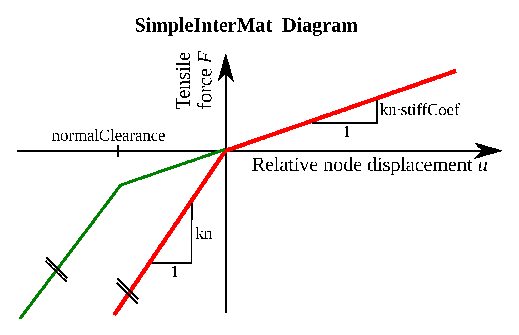
\includegraphics[width=0.7\textwidth]{Simple_interface_material_diag.eps}}
\end{htmlonly}
%begin{latexonly}
 \centerline{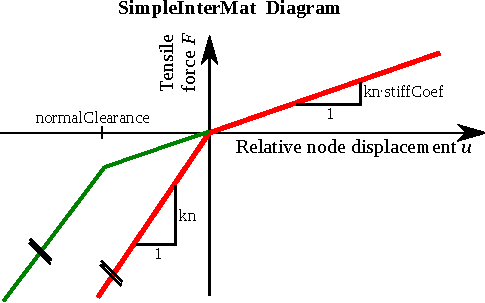
\includegraphics[width=0.7\textwidth]{Simple_interface_material_diag}}
%end{latexonly}
  \caption{Working diagram of SimpleInterfaceMat.}
  \label{SimpleInterfaceMat}
\end{figure}

\subsection{Material models for lattice elements}

Lattice elements have to be used with material models describing the constitutive behavior in the form of vector of  tractions and strains determined from displacement jumps smeared out over the element length.

\subsubsection{Latticedamage2d}
This is a damage lattice material used together with latticedamage2d elements.
It uses a scalar damage relationship of the form
\begin{equation}
\boldsymbol{\sigma} = \left(1-\omega\right) \mathbf{D}_{\rm e} \boldsymbol{\varepsilon}
\end{equation}
where $\boldsymbol{\sigma} = \left( \sigma_{\rm n}, \sigma_{\rm t}, \sigma_{\rm \phi}\right)^{T}$ is a vector of tractions and $\boldsymbol{\varepsilon} = \left( \varepsilon_{\rm n}, \varepsilon_{\rm t}, \varepsilon_{\rm \phi}\right)^{T}$ is a vector of strains obtained from displacement jumps smeared over the element length.
Furthermore, $\omega$ is the damage variable varying from 0 (undamaged) to 1 (fully damaged). 
Also, $\mathbf{D}_{\rm e}$ is the elastic stiffness matrix which is based on the elastic modulus of the lattice material $E$, and a parameter $\gamma$ which is the ratio of the modulus of the shear and normal direction.
The strength envelope is elliptic (Figure~\ref{StrengthLatticeDamage2d}) and determined by three  parameters, $f_{\rm t}$, $f_{\rm q}$ and $f_{\rm c}$. The evolution of the damage variable $\omega$ is controlled by normal stress-normal crack opening law. The three possible laws are linear, bilinear and exponential (Figure~\ref{SofteningLatticeDamage2d}).

\begin{figure}[!htb]
\begin{htmlonly}
  \centerline{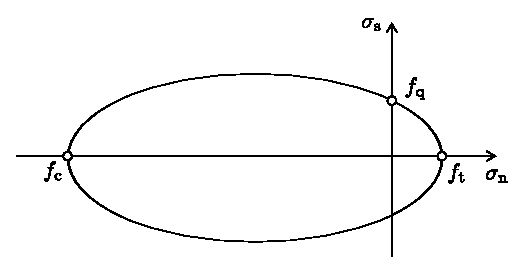
\includegraphics[width=0.7\textwidth]{figStrengthLatticeDamage2d.eps}}
\end{htmlonly}
%begin{latexonly}
 \centerline{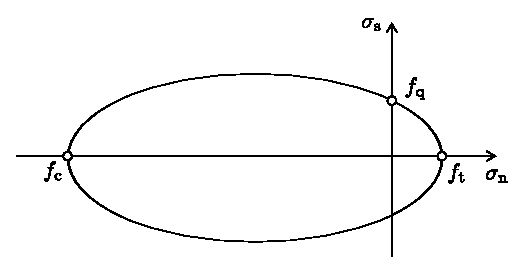
\includegraphics[width=0.7\textwidth]{figStrengthLatticeDamage2d}}
%end{latexonly}
  \caption{Strength envelope of LatticeDamage2d.}
  \label{StrengthLatticeDamage2d}
\end{figure}


\begin{figure}[!htb]
\begin{tabular}{ccc}
\begin{htmlonly}
  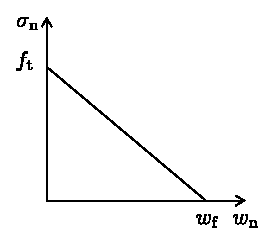
\includegraphics[width=0.7\textwidth]{figSofteningLatticeDamage2da.eps} & 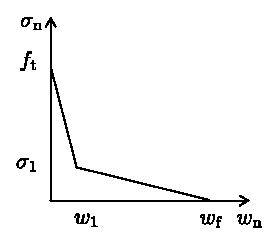
\includegraphics[width=0.7\textwidth]{figSofteningLatticeDamage2db.eps} & 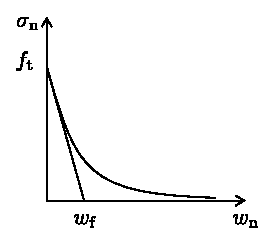
\includegraphics[width=0.7\textwidth]{figSofteningLatticeDamage2dc.eps}\\
\end{htmlonly}
%begin{latexonly}
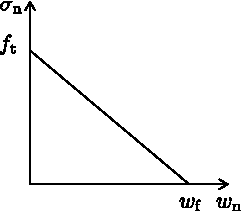
\includegraphics[width=0.3\textwidth]{figSofteningLatticeDamage2da} & 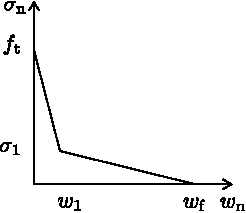
\includegraphics[width=0.3\textwidth]{figSofteningLatticeDamage2db} & 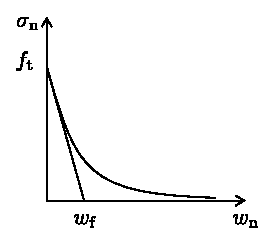
\includegraphics[width=0.3\textwidth]{figSofteningLatticeDamage2dc}\\
%end{latexonly}
(a) & (b) & (c)
\end{tabular}
  \caption{Softening types of LatticeDamage2d: (a) linear softening, (b) bilinear softening, (c) exponential softening.}
  \label{SofteningLatticeDamage2d}
\end{figure}

The model parameters are summarised in Tab.~\ref{latticedamage2d_table}.
\begin{table}[!htb]
%\begin{center}
\begin{tabular}{|l|p{9cm}|}
\hline
Description & Saclar damage model for lattice2d \\
\hline
Record Format & \descitem{latticedamage2d} \elemparam{}{in} 
\elemparam{d}{rn} \elemparam{talpha}{rn} \elemparam{e}{rn} \elemparam{a1}{rn} \elemparam{a2}{rn} \elemparam{e0}{rn}  \elemparam{coh}{rn} \elemparam{ec}{rn} \elemparam{stype}{rn} \elemparam{wf}{rn} \elemparam{wf1}{rn} \\
Parameters &- \param{} material number\\
&- \param{d} material density\\
&- \param{talpha} Thermal exansion coefficient\\
&- \param{e} normal modulus of lattice material\\
&- \param{a1} ratio of shear and normal modulus\\
&- \param{a2} ratio of rotational and normal modulus. Optional parameter. Default is 1.\\
&- \param{e0} strain at tensile strength: $f_{\rm t}/E$\\
&- \param{coh} ratio of shear and tensile strength: $f_{\rm q}/f_{\rm t}$\\
&- \param{ec} ratio of compressive and tensile strength: $f_{\rm c}/f_{\rm t}$\\
&- \param{stype} softening types: 1-linear, 2-bilinear and 3-exponential\\
&- \param{wf} displacement threshold related to fracture energy used in all three softening types.\\

Supported modes& 2dlattice\\
\hline
\end{tabular}
\caption{Scalar damage model for 2d lattice elements -- summary.}
\label{latticedamage2d_table}
%\end{center}
\end{table}

\clearpage

\section{Material Models for Transport Problems}
\subsection{Isotropic linear material for heat transport -- IsoHeat}
\label{IsoLET}
Linear isotropic material model for heat transport problems described
by the linear diffusion equation
\begin{equation}\label{lindiffheat}
c\frac{\partial T}{\partial t} = \nabla \cdot \left( k \nabla T \right)
\end{equation}
where $T$ is the temperature, $c$ is the specific heat capacity,
and $k$ is the conductivity.
The model parameters are summarized
in Tab.~\ref{Isoheat_table}.

\begin{table}[!htb]
%\begin{center}
\begin{tabular}{|l|p{9cm}|}
\hline
Description & Linear isotropic elastic material\\
\hline
Record Format & \descitem{IsoHeat} \elemparam{num}{in}
\elemparam{d}{rn} \elemparam{k}{rn} \elemparam{c}{rn}\\
Parameters &- \param{num} material model number\\
&- \param{d} material density\\
&- \param{k} Conductivity\\
&- \param{c} Specific heat capacity\\
Supported modes& \_2dHeat\\
\hline
\end{tabular}
\caption{Linear isotropic material for heat transport - summary.}
\label{Isoheat_table}
%\end{center}
\end{table}


\subsection{Isotropic linear material for moisture transport -- IsoLinMoisture}
\label{IsoLinMoistureMat}
Linear isotropic material model for moisture transport problems described
by the linear diffusion equation\footnote{Note that the symbols $k$ and $c$
in \refeq{lindiff} have a different meaning than in \refeq{lindiffheat}.
The reason is that the nonlinear model for moisture transport described
in Section \ref{sec:NlIsoMoistureMat} traditionally
uses $c$ for permeability and \refeq{lindiff} should be obtained
as a special case of \refeq{nlisomoisture:governing}. 
On the other hand, the heat conduction model
from Section \ref{IsoLET} was implemented earlier and the input parameters
are directly called $k$ and $c$, so changing this notation now could lead
to confusion for some older input files.}
\begin{equation}\label{lindiff}
k\frac{\partial h}{\partial t} = \nabla \cdot \left( c \nabla h \right)
\end{equation}
where $h$ is the pore relative humidity (dimensionless, between 0 and 1), 
$k$ is the moisture capacity [kg/m$^3$],
and $c$ is the moisture permeability [kg/m$\cdot$s].
The model parameters are summarized
in Tab.~\ref{IsoLinmoistureMat_table}.

\begin{table}[!htb]
%\begin{center}
\begin{tabular}{|l|p{9cm}|}
\hline
Description & Linear isotropic material for moisture transport\\
\hline
Record Format & \descitem{IsoLinMoistureMat} \elemparam{num}{in}
\elemparam{d}{rn} \elemparam{perm}{rn} \elemparam{capa}{rn}\\
Parameters &- \param{num} material model number\\
&- \param{d} material density\\
&- \param{perm} moisture permeability\\
&- \param{capa} moisture capacity\\
Supported modes& \_2dHeat\\
\hline
\end{tabular}
\caption{Linear isotropic material for moisture transport - summary.}
\label{IsoLinmoistureMat_table}
%\end{center}
\end{table}

\subsection{Isotropic material for moisture transport based on Ba\v{z}ant
  and Najjar -- BazantNajjarMoisture}
\label{sec:BazantNajjarMoistureMat}
This is a specific model for nonlinear moisture transport in isotropic cementitious
materials, based on \cite{Bazant:72}.
The governing equation 
\begin{equation}\label{BNmodel:governing}
\frac{\partial h}{\partial t} = \nabla \cdot \left( C(h) \nabla h \right)
\end{equation} 
is a special case of \refeq{nlisomoisture:governing}, valid under
the assumption that the slope of the sorption isotherm is linear, i.e.\ the
moisture capacity is constant.
In \refeq{BNmodel:governing}, $h$ is the relative humidity and $C(h)$ is the
humidity-dependent diffusivity approximated by
\begin{equation}\label{BNmodel:diffusivity}
C (h) = C_1 \left( \alpha_0
+ \frac{1-\alpha_0}{1+\left(\frac{1-h}{1-h_c}\right)^n} \right)
\end{equation}
where $C_1$ is the diffusivity at saturation (typical value for concrete
$\approx 30$ mm$^2/$day), $\alpha_0$ is the dimensionless ratio of
diffusivity at low humidity to diffusivity at saturation (typical
value $\approx 0.05$), $h_c$ is the humidity ``in the middle'' of the
transition between low and high diffusivity (typical value $\approx 0.8$), and $n$ is dimensionless
exponent (high values of $n$, e.g.\ 12, lead to a rapid transition
between low and high diffusivity). Optionally, it is possible to
specify the moisture capacity. This property is not needed for solution
of the diffusion equation  (\ref{BNmodel:governing}),
but it is needed if the computed change of relative humidity is transformed     
into water content loss (mass of lost water per unit volume).

The model parameters are summarized in Tab.~\ref{BazantNajjarMoistureMat}.
\begin{table}[!htb]
%\begin{center}
\begin{tabular}{|l|p{9cm}|}
\hline
Description & Nonlinear isotropic material for moisture transport\\
\hline
Record Format & \descitem{BazantNajjarMoistureMat} \elemparam{num}{in}
\elemparam{d}{rn} \elemparam{c1}{rn} \elemparam{n}{rn}
\elemparam{alpha0}{rn} \elemparam{hc}{rn} \optelemparam{capa}{rn}\\
Parameters &- \param{num} material model number\\
&- \param{d} material density\\
&- \param{c1} moisture diffusivity at full saturation [m$^2$ s$^{-1}$]\\
&- \param{n} exponent [-]\\
&- \param{alpha0} ratio between minimum and maximum diffusivity [-]\\
&- \param{hc} relative humidity at which the diffusivity is exactly
between its minimum and maximum value [-] \\
&- \param{capa} moisture capacity (default value is 1.0)\\

Supported modes& \_2dHeat\\
\hline
\end{tabular}
\caption{Nonlinear isotropic material for moisture transport - summary.}
\label{BazantNajjarMoistureMat}
%\end{center}
\end{table}



\subsection{Nonlinear isotropic material for moisture transport -- NlIsoMoisture}
\label{sec:NlIsoMoistureMat}
This is a more general model for nonlinear moisture transport in isotropic 
porous
materials, based on a nonlinear sorption isotherm (relation between 
the pore relative humidity $h$ and the water content $w$) 
and on a humidity-dependent
moisture permeability.
The governing differential equation reads
\begin{equation}\label{nlisomoisture:governing}
k(h) \frac{\partial h}{\partial t} = \nabla \cdot \left[ c(h) \nabla h \right]
\end{equation} 
where 
$k(h)$ [kg/m$^3$] is the humidity-dependent moisture capacity (derivative of
the moisture content with respect to the relative humidity), and $c(h)$
[kg/m$\cdot$s] is the moisture permeability. 

So far, six different functions for the {\bf sorption
isotherm} have been implemented  (in fact, what matters for the model
is not the isotherm itself but its derivative---the moisture capacity):
\begin{enumerate}

\item
{\bf Linear} isotherm ($isothermType=0$) is characterized only by its
slope given by parameter $moistureCapacity$.

\item
{\bf Piecewise linear} isotherm ($isothermType=1$) is defined by two 
arrays
with the values of pore relative humidity $iso\_h$ and the
corresponding values of moisture content $iso\_w(h)$. The arrays must be of
the same size. 

\item
{\bf Ricken} isotherm \cite{Kuenzel}
($isothermType=2$), which is widely used for sorption of porous building
materials. It is
expressed by the equation
\begin{equation}\label{nlisomoisture:ricken}
w(h) = w_0 - \frac{\ln(1-h)}{d}
\end{equation} 
where $w_0$ [kg/m$^3$] is the water content at $h=0$ and $d$ [m$^3$/kg] is
an approximation coefficient. In the input record, only $d$ must be specified 
($w_0$ is not needed). Note that for $h=1$ this isotherm
gives an infinite moisture content. 

\item
Isotherm proposed by {\bf Kuenzel} \cite{Kuenzel} ($isothermType=3$) 
in the form 
\begin{equation}\label{nlisomoisture:kuenzel}
w(h) = w_f \frac{(b-1)h}{b-h}
\end{equation} 
where $w_f$ [kg/m$^3$] is the moisture content at free saturation and
$b$ is a dimensionless approximation factor greater than 1.

\item
Isotherm proposed by {\bf Hansen} \cite{Hansen} ($isothermType=4$) in the form
\begin{equation}\label{nlisomoisture:hansen}
u(h) = u_h \left(1- \frac{\ln h}{A} \right)^{-1/n}
\end{equation} 
characterizes the amount of adsorbed water 
by the moisture ratio $u$ [kg/kg]. To obtain the
moisture content $w$, it is necessary to multiply the moisture ratio
by the density of the solid phase. In (\ref{nlisomoisture:hansen}),
 $u_h$ is the maximum hygroscopically
bound water by adsorption, and $A$ and $n$ are constants
obtained by fitting of experimental data.

\item
The {\bf BSB} isotherm \cite{BSB} ($isothermType=5$) is an improved
version of the famous BET isotherm. It is expressed in terms
of the moisture ratio
\begin{equation}\label{nlisomoisture:BSB}
u(h) = \frac{C k V_m h}{(1-k h)(1+(C-1)k h)}
\end{equation} 
where $V_m$ is the monolayer capacity, and $C$ depends on the absolute
temperature $T$ and on the difference between the heat of adsorption and
condensation. Empirical formulae for estimation of the parameters can
be found in \cite{Xi}. Note that these formulae hold quite accurately
for cement paste only; a reduction of the moisture ratio is necessary 
if the isotherm
should be applied for concrete. 
\end{enumerate}

The present implementation covers three functions for 
{\bf moisture permeability}:
\begin{enumerate}

\item
{\bf Piecewise linear} permeability  ($permeabilityType=0$) 
is defined by two arrays
with the values of pore relative humidity $perm\_h$ and the
corresponding values of moisture content $perm\_c(h)$. The arrays must be of
the same size. 

\item
The {\bf Ba\v{z}ant-Najjar} 
permeability function ($permeabilityType=1$) is given by the same
formula (\ref{BNmodel:diffusivity}) as the diffusivity in 
Section \ref{sec:BazantNajjarMoistureMat}. All parameters have a similar
meaning as in (\ref{BNmodel:diffusivity}) but  $c1$ is now the
moisture permeability at full saturation [kg/m$\cdot$s].

\item
Permeability function proposed by {\bf Xi et al.} \cite{Xi}
($permeabilityType=2$) reads
\begin{equation}\label{nlisomoisture:Xi}
c(h) = \alpha_h + \beta_h \left[ 1 - 2^{-10^{\gamma_h(h-1)}} \right]
\end{equation} 
where $\alpha_h$, $\beta_h$ and $\gamma_h$ are parameters that can be
evaluated using empirical mixture-based formulae presented in \cite{Xi}. 
However, if those formulae are used outside the range of water-cement 
ratios for which they were calibrated, the
permeability may become negative. Also the physical units are unclear.
\end{enumerate}

Note that the Bajant-Najjar 
model from Section \ref{sec:BazantNajjarMoistureMat} 
can be obtained as a special
case of the present model if $permeabilityType$ is set to 1
and $isothermType$ is set to 0. 
The ratio $c1/moistureCapacity$ then corresponds to the diffusivity
parameter $C_1$ from \refeq{BNmodel:governing}.

The model parameters are summarized in Tab.~\ref{NlIsoMoistureMat}.
\begin{table}[!htb]
%\begin{center}
\begin{tabular}{|l|p{9cm}|}
\hline
Description & Nonlinear isotropic material for moisture transport \\
\hline
Record Format & \descitem{NlIsoMoistureMat} \elemparam{num}{in}
\elemparam{d}{rn} \elemparam{isothermType}{in} \elemparam{permeabilityType}{in}
\optelemparam{rhodry}{rn} \optelemparam{capa}{rn}
\optelemparam{iso\_h}{ra} \optelemparam{iso\_w(h)}{ra}
\optelemparam{dd}{rn} \optelemparam{wf}{rn} \optelemparam{b}{rn}
\optelemparam{uh}{rn} \optelemparam{A}{rn} \optelemparam{nn}{rn}
\optelemparam{c}{rn} \optelemparam{k}{rn} \optelemparam{Vm}{rn}
\optelemparam{perm\_h}{ra} \optelemparam{perm\_c(h)}{ra}
\optelemparam{c1}{rn} \optelemparam{n}{rn} \optelemparam{alpha0}{rn}
\optelemparam{hc}{rn} \optelemparam{alphah}{rn}
\optelemparam{betah}{rn} \optelemparam{gammah}{rn} \\
Parameters &- \param{num} material model number \\
&- \param{d} material density \\
&- \param{isothermType} isotherm function as listed above (0, 1, ...5)
\\
&- \param{permeabilityType} moisture permeability function as listed
above (0, 1, 2) \\
&- \param{rhodry} [kg/m$^3$] density of dry material (for $isothermType=4$ and 5) \\
&- \param{capa} [kg/m$^3$] moisture capacity (for $isothermType=0$) \\
&- \param{iso\_h} [-] humidity array (for $isothermType=1$) \\
&- \param{iso\_w(h)} [kg/m$^3$] moisture content array (for
$isothermType=1$) \\
&- \param{dd} [-] parameter (for $isothermType=2$)\\
&- \param{wf} [kg/m$^3$] is the moisture content at free saturation
(for $isothermType=3$) \\
&- \param{b} [-] parameter (for $isothermType=3$) \\
&- \param{uh} [kg/kg] maximum hygroscopically
bound water by adsorption (for $isothermType=4$) \\
&- \param{A} [-] parameter (for $isothermType=4$) \\
&- \param{n} [-] parameter (for $isothermType=4$) \\
&- \param{Vm} (for $isothermType=5$) \\
&- \param{k} (for $isothermType=5$) \\
&- \param{C} (for $isothermType=5$) \\
&- \param{perm\_h} [-] humidity array (for $permeabilityType=0$) \\
&- \param{perm\_c(h)} [kg m$^{-1}$ s$^{-1}$] moisture permeability
array (for $permeabilityType=0$) \\
&- \param{c1} [kg m$^{-1}$ s$^{-1}$] moisture permeability at full
saturation (for $permeabilityType=1$) \\
&- \param{n} [-] exponent (for $permeabilityType=1$) \\
&- \param{alpha0} [-] ratio between minimum and maximum diffusivity
(for $permeabilityType=1$) \\
&- \param{hc} [-] relative humidity at which the diffusivity is exactly
between its minimum and maximum value (for $permeabilityType=1$) \\
&- \param{alphah} [kg m$^{-1}$ s$^{-1}$] (for $permeabilityType=2$) \\
&- \param{betah} [kg m$^{-1}$ s$^{-1}$] (for $permeabilityType=2$) \\
&- \param{gammah} [-] (for $permeabilityType=2$) \\

Supported modes& \_2dHeat \\
\hline
\end{tabular}
\caption{Nonlinear isotropic material for moisture transport - summary.}
\label{NlIsoMoistureMat}
%\end{center}
\end{table}



\subsection{Material for cement hydration - CemhydMat}
\label{Cemhyd}
CemhydMat represents a hydrating material based on CEMHYD3D model version 3.0,
developed at NIST \cite{NISTIR7232}. The model represents a digital hydrating
microstructure, driven with cellular automata rules and combined with cement
chemistry. Ordinary Portland cement is treated without any difficulties, blended
cements are ususally decomposed into hydrating Portland contribution and intert
secondary cementitious material. The microstructure size can be from
$10\times10\times10$ to over $200\times200\times200$~$\mu$m. For standard
computations the size $50\times50\times50$ suffices.

Each material instance creates an independent microstructure. It is also
possible to enforce having different microstructures in each integration point.
The hydrating model is coupled with temperature and averaging over shared
elements within one material instance occurs during the solution. Such approach
allows domain partitioning to many CemhydMat instances, depending on expected
accuracy or computational speed. A more detailed description with engineering
examples was published \cite{Smilauer:09}. Tab.~\ref{Cemhydmat_table} summarizes input parameters.

\begin{table}[!htb]
%\begin{center}
\begin{tabular}{|l|p{9cm}|}
\hline
Description & Cemhyd - hydrating material\\
\hline
Record Format & \descitem{CemhydMat} \elemparam{num}{in} \elemparam{d}{rn} \elemparam{k}{rn} \elemparam{c}{rn} \elemparam{file}{s} [\elemparam{eachGP}{in}] [\elemparam{densityType}{in}] [\elemparam{conductivityType}{in}] [\elemparam{capacityType}{in}] [\elemparam{castingtime}{rn}] [\elemparam{nowarnings}{ia}] [\elemparam{scaling}{ra}] [\elemparam{reinforcementDegree}{rn}]\\
Parameters &- \param{num} material model number\\
&- \param{d} material density\\
&- \param{k} Conductivity\\
&- \param{c} Specific heat capacity\\
&- \param{file} XML input file for cement microstructure and concrete composition\\
&- \param{eachGP} 0 (default) no separate microstructures in each GP, 1 assign separate microstructures to each GP\\
&- \param{densityType} 0 (default) get density from OOFEM input file, 1 get it from XML input file\\
&- \param{conductivityType} 0 (default) get constant conductivity from OOFEM input file, 1 compute as $\lambda = \textrm{k} (1.33-0.33\alpha)$ \cite{Ruiz:01}\\
&- \param{capacityType} 0 (default) get capacity, 1 according to Bentz, 2 according to XML and CEMHYD3D routines\\
&- \param{castingtime} optional casting time of concrete, from which hydration takes place. Absolute time is used.\\
&- \param{nowarnings} supresses warnings when material data are out of standard ranges. The array of size 4 represent entries for density, conductivity, capacity, temperature. Nonzero values mean supression.\\
&- \param{scaling} components in the array scale density, conductivity, capacity in this order. \param{nowarnings} are checked before scaling.\\
&- \param{reinforcementDegree} specifies the area fraction of reinforcement. Typical values is 0.015. Steel reinforcement slightly increases concrete conductivity and slightly decreases its capacity. Thermal properties of steel are considered 20~W/m/K and 500~J/kg/K.\\
Supported modes& \_2dHeat, \_3dHeat\\
\hline
\end{tabular}
\caption{Cemhydmat - summary.}
\label{Cemhydmat_table}
%\end{center}
\end{table}

The input XML file specifies the details about cement and concrete composition.
It is possible to start all simulations from the scratch, i.e. with the
reconstruction of digital microstructure. Alternatively, the digital
microstructure can be provided directly in two files; one for chemical phases,
the second for particle's IDs. The XML input file can be created with the CemPy
package, obtainable from
http://mech.fsv.cvut.cz/$\sim$smilauer/index.php?id=software. The CemPy package
alleviates tedious preparation of particle size distribution etc.

The linear solver (specified as NonStationaryProblem) performs well when the
time integration step is small enough (order of minutes) and heat capacity,
conductivity and density remain constant. If not so, use of nonlinear solver is
strongly suggested (specified as NlTransientTransportProblem).

\clearpage

\subsection{Material for cement hydration - HydratingConcreteMat}
\label{Affinity1}
Simple hydration models based on chemical affinity are implemented. The models calculate degree of hydration of cement, $\alpha$, which can be scaled to the level of concrete when providing corresponding amount of cement in concrete. Blended cements can be considered as well, either by separating supplementary cementitious materials from pure Portland clinker or by providing parameters for the evolution of hydration degree and potential heat. Released heat from cement paste is obtained from
\begin{eqnarray}
Q(t) = \alpha Q_{pot},
\end{eqnarray}
where potential hydration heat, $Q_{pot}$, is expressed in kJ/kg of cement and for pure Portland cement is around 500 kJ/kg.

Evolution of hydration degree under isothemal curing conditions is approximated by several models. Scaling from a reference temperature to arbitrary temperature is based on Arrhenius equation, which coincides with the maturity method approach. The equivalent time, $t_e$, is defined as time under constant reference (isothermal) temperature
\begin{eqnarray}
t_e(T_0)&=&t(T) k_{rate},\\
k_{rate}&=&\exp\left[\frac{E_a}{R}\left(\frac{1}{T_0}-\frac{1}{T}\right)\right],
\end{eqnarray}
where $t$ is real time, $T$ is the arbitrary constant temperature of hydration, $T_0$ is a reference temperature, $R$ is the universal gas constant (8.314 Jmol$^{-1}$K$^{-1}$) and $E_a$ is the apparent activation energy. Due to varying history of temperature, incremental solution is adopted. Linear and nonlinear nonstationary solvers are supported for all \param{hydrationmodeltype}'s. Hydration models are evaluated at intrinsic time in each time step. Usually, intrinsic time is in the middle of the time step.

The \param{hydrationmodeltype} = 1 is based on exponential approximation of hydration degree \cite{Schindler:2005}. Equivalent time increment is added in each time step. Thus all the thermal history is stored in the equivalent time
\begin{eqnarray}
\alpha(t_e) &=& \alpha_\infty \exp\left(-\left[\frac{\tau}{t_e} \right]^\beta \right)\label{eq:affinity1}
%\frac{\ud \alpha(t)}{\ud t} &=& \frac{b\alpha_\infty}{t} \left( \frac{\tau}{t} \right)^\beta \exp\left(-\left[\frac{\tau}{t} \right]^\beta \right)
\end{eqnarray}
where three parameters $\tau$, $\beta$ and $\alpha_\infty$ are needed. Some meaningful parameters are provided in \cite{Schindler:2005}, e.g. $\tau=26\cdot3600=93600$~s, $\beta=0.75$ and $\alpha_\infty=0.90$.

The \param{hydrationmodeltype} = 2 is inspired by Cervera et al. \cite{Cervera:99}, who proposed an analytical form of the normalized affinity which was refined in \cite{Gawin:06a}. A slightly modified formulation is proposed here. The affinity model is formulated for a reference temperature 25\C
\begin{eqnarray}
\frac{\ud \alpha}{\ud t} = \tilde{A}_{25}(\alpha) k_{rate}= B_1 \left( \frac{B_2}{\alpha_\infty} + \alpha \right ) \left( \alpha_\infty - \alpha \right) \exp\left(-\bar{\eta}\frac{\alpha}{\alpha_\infty}\right) k_{rate} \label{eq:affinity2}
\end{eqnarray}
where $B_1, B_2$ are coefficients to be calibrated, $\alpha_\infty$ is the ultimate hydration degree and $\bar{\eta}$ represents microdiffusion of free water through formed hydrates. The solution proceeds incrementally, where $\alpha$ is the unknown. During one macroscopic time step, \refeq{eq:affinity2} needs to be integrated in finer inner steps. This is controlled with two optional variables; \param{maxmodelintegrationtime} specifies maximum integration time in the loop while \param{minmodeltimestepintegrations} specifies minimum number of integration steps.

\begin{table}[!htb]
%\begin{center}
\begin{tabular}{|l|p{9cm}|}
\hline
Description & HydratingConcreteMat\\
\hline
Record Format & \descitem{HydratingConcreteMat} \elemparam{num}{in} \elemparam{d}{rn} \elemparam{k}{rn} \elemparam{c}{rn} \elemparam{hydrationmodeltype}{in} \elemparam{Qpot}{rn} \elemparam{masscement}{rn} [\elemparam{activationenergy}{rn}] \elemparam{reinforcementdegree}{rn}] [\elemparam{densitytype}{in}] [\elemparam{conductivitytype}{in}] [\elemparam{capacityType}{in}]   [\elemparam{minModelTimeStepIntegrations}{in}]  [\elemparam{maxmodelintegrationtime}{rn}] [\elemparam{castingTime}{rn}]\\
Parameters &- \param{num} material model number\\
&- \param{d} material density about 2300 kg/m$^3$\\
&- \param{k} Conductivity about 1.7 W/m/K\\
&- \param{c} Specific heat capacity about 870 J/kg/K\\
&- \param{hydrationmodeltype} 1 is exponential model from \refeq{eq:affinity1}, 2 is affinity model from \refeq{eq:affinity2}\\
&- \param{Qpot} Potential heat of hydration, about 500 kJ/kg of cement\\
&- \param{masscement} Cement mass per 1m$^3$ of concrete, about 200-450\\
&- \param{activationenergy} Arrhenius activation energy, 38400. (default)\\
&- \param{reinforcementDegree} specifies the area fraction of reinforcement. Typical values is 0.015. Steel reinforcement slightly increases concrete conductivity and slightly decreases its capacity. Thermal properties of steel are considered 20~W/m/K and 500~J/kg/K.\\
&- \param{densityType} 0 (default)\\
&- \param{conductivityType} 0 (default), 1 compute as $\lambda = \textrm{k} (1.33-0.33\alpha)$ \cite{Ruiz:01}\\
&- \param{capacityType} 0 (default)\\
&- \param{minModelTimeStepIntegrations} Minimum integrations per time step in affinity model 30 (default)\\
&- \param{maxmodelintegrationtime} Maximum integration time step in affinity model 36000 s (default)\\
&- \param{castingtime} optional casting time of concrete, from which hydration takes place, in s\\
&- \param{scaling} components in the array scale density, conductivity, capacity in this order. \param{nowarnings} are checked before scaling.\\
Supported modes& \_2dHeat, \_3dHeat\\
\hline
\end{tabular}
\caption{HydratingConcreteMat - summary of affinity hydration models.}
\label{Affinity1_table}
%\end{center}
\end{table}

\reffig{hydration_comparison} shows mutual comparison of three hydration models implemented in OOFEM. Parameters for exponential model according to \refeq{eq:affinity1} are $\tau=26\cdot3600=93600$~s, $\beta=0.75$, $\alpha_\infty=0.90$. Parameters for affinity model according to \refeq{eq:affinity2} are $B_1=3.519e-4$~s$^{-1}$, $B_2=8.0e-7$, $\eta=7.4$, $\alpha_\infty=0.85$.

\begin{figure}[!htb]
\begin{htmlonly}
  \centerline{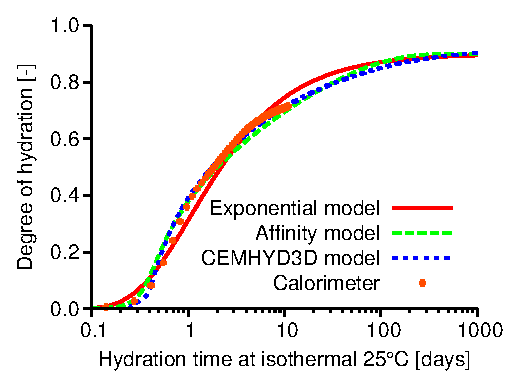
\includegraphics[width=0.7\textwidth]{Mokra_OOFEM_affinity_time.eps}}
\end{htmlonly}
%begin{latexonly}
 \centerline{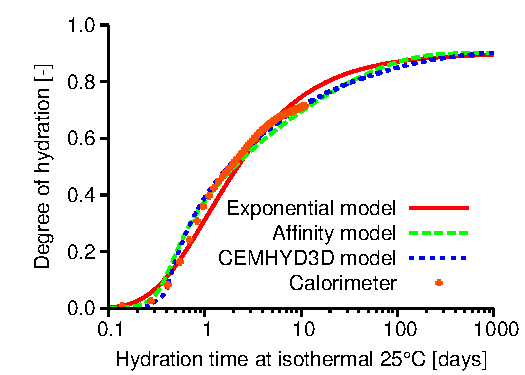
\includegraphics[width=0.7\textwidth]{Mokra_OOFEM_affinity_time}}
%end{latexonly}
  \caption{Performance of implemented hydration models: exponential model from \refeq{eq:affinity1}, affinity model from \refeq{eq:affinity2}, CEMHYD3D model from Subsection~\ref{Cemhyd}.}
  \label{hydration_comparison}
\end{figure}


\subsection{Coupled heat and mass transfer material model - HeMotk}
Coupled heat and mass transfer material model.
Source: T. Krejci doctoral thesis; Bazant and Najjar, 1972;
Pedersen, 1990. Assumptions: water vapor is the only driving
mechanism; relative humidity is from range 0.2 - 0.98 (I and II
regions). The model parameters are summarized
in Tab.~\ref{hemotk_table}.
\begin{table}[!htb]
%\begin{center}
\begin{tabular}{|l|p{9cm}|}
\hline
Description & Coupled heat and mass transfer material model\\
\hline
Record Format & \descitem{HeMotk} \elemparam{num}{in}
\elemparam{d}{rn} \elemparam{a\_0}{rn} \elemparam{nn}{rn}
\elemparam{phi\_c}{rn} \elemparam{delta\_wet}{rn}
\elemparam{w\_h}{rn} \elemparam{n}{rn}
\elemparam{a}{rn} \elemparam{latent}{rn}
\elemparam{c}{rn} \elemparam{rho}{rn}
\elemparam{chi\_eff}{rn} \elemparam{por}{rn}
\elemparam{rho\_gws}{rn}\\
Parameters &- \param{num} material model number\\
&- \param{d}, \param{rho} material density\\
&- \param{a\_0} constant (obtained from experiments) a\_0 [Bazant and Najjar, 1972]\\
&- \param{nn} constant-exponent (obtained from experiments) n [Bazant
and Najjar, 1972]\\
&- \param{phi\_c} constant-relative humidity  (obtained from experiments) phi\_c [Bazant and Najjar, 1972]\\
&- \param{delta\_wet} constant-water vapor permeability (obtained from
experiments) delta\_wet [Bazant and Najjar, 1972]\\
&- \param{w\_h} constant water content (obtained from experiments) w\_h
[Pedersen, 1990]\\
&- \param{n} constant-exponent (obtained from experiments) n [Pedersen, 1990]\\
&- \param{a} constant (obtained from experiments) A [Pedersen, 1990]\\
&- \param{latent} latent heat of evaporation\\
&- \param{c} thermal capacity\\
&- \param{chi\_eff} effective thermal conductivity\\
&- \param{por} porosity\\
&- \param{rho\_gws} saturation volume density\\
Supported modes& \_2dHeMo\\
\hline
\end{tabular}
\caption{Coupled heat and mass transfer material model - summary.}
\label{hemotk_table}
%\end{center}
\end{table}

\clearpage

\section{Material Models for Fluid Dynamic}
\subsection{Newtonian fluid - NewtonianFluid}
\label{NewtonianFluidMaterial}
Constitutive model of Newtonian fluid. The model parameters are summarized
in Tab.~\ref{NewtonianFluidMaterial_table}.

\begin{table}[!htb]
%\begin{center}
\begin{tabular}{|l|p{9cm}|}
\hline
Description & Newtonian Fluid material\\
\hline
Record Format & \descitem{NewtonianFluid} \elemparam{num}{in}
\elemparam{d}{rn} \elemparam{mu}{rn}\\
Parameters &- \param{num} material model number\\
&- \param{d} material density\\
&- \param{mu} viscosity\\
Supported modes& 2d, 3d flow\\
\hline
\end{tabular}
\caption{Newtonian Fluid material - summary.}
\label{NewtonianFluidMaterial_table}
%\end{center}
\end{table}



\subsection{Bingham fluid - BinghamFluid}
\label{BinghamFluidMaterial}
Constitutive model of Bingham fluid. This is a constitutive model of
non-Newtonian type. The model parameters are summarized
in Tab.~\ref{BinghamFluidMaterial_table}.

In the Bingham model the flow is characterized by following
constitutive equation
\begin{eqnarray}
  \label{eq:bigham-model}
  \mbf{\tau}&=&\mbf{\tau}_0+\mu\mbf{\dot\gamma}\;\;\;\rm{if}\
  \dot\tau\ge\tau_0\\
  \dot\gamma &=& \mbf{0}\;\;\;\;\;\;\;\;\;\;\;\;\;\;\rm{if}\ \dot\tau\le\tau_0
\end{eqnarray}
where $\mbf{\tau}$ is the shear stress applied to material, $\dot\tau=\sqrt{\mbf{\tau}:\mbf{\tau}}$
is the shear stress measure, $\mbf{\dot\gamma}$ is
the shear rate, $\mbf{\tau}_0$ is the yield stress, and $\mu$ is the plastic
viscosity.
The parameters for the model can be in general determined using two
possibilities: (i) stress controlled rheometer, when the stress is applied
to material and shear rate is measured, and (ii) shear rate controlled
rheometer, where concrete is sheared and stress is measured. However,
most of the widely used tests are unsatisfactory in the sense, that
they measure only one parameter. These one-factor tests include slump
test, penetrating rod test, and Ve-Be test. Recently, some tests
providing two parameters on output have been designed (BTRHEOM, IBB,
and BML rheometers). Also a refined version of the
standard slump test has been developed for estimating yield stress and
plastic viscosity. The test is based on measuring the time necessary
for the upper surface of the concrete cone in the slump to fall a
distance 100 mm. Semi-empirical models are then proposed for estimating
yield stress and viscosity based on measured results. The advantage
is, that this test does not require any special equipment, provided that
the one for the standard version is available.

In order to avoid numerical difficulties caused by the existence of
the sharp angle in material model
response at $\tau=\tau_0$, the numerical implementation uses
following smoothed relation for viscosity
\begin{equation}
\label{eq:smooth-bigham-model}
\mu=\mu_0+\del{\tau_0}{\dot\gamma}(1-e^{-m\dot\gamma})
\end{equation}
where $m$ is so called stress growth parameter. The higher value of
parameter $m$, the closer approximation of the original
constitutive equation (\ref{eq:bigham-model}) is obtained.
%
%In practical simulations, it is usually taken $m=5000$.
%

\begin{table}[!htb]
%\begin{center}
\begin{tabular}{|l|p{9cm}|}
\hline
Description & Bingham fluid material\\
\hline
Record Format & \descitem{BinghamFluid} \elemparam{num}{in}
\elemparam{d}{rn} \elemparam{mu0}{rn} \elemparam{tau0}{rn}\\
Parameters &- \param{num} material model number\\
&- \param{d} material density\\
&- \param{mu0} viscosity\\
&- \param{tau0} Yield stress\\
Supported modes& 2d, 3d flow\\
\hline
\end{tabular}
\caption{Bingham Fluid material - summary.}
\label{BinghamFluidMaterial_table}
%\end{center}
\end{table}



\subsection{Two-fluid material - TwoFluidMat}
\label{TwoFluidMaterial}
Material coupling the behaviour of two particulat materials based on
rule of mixture. The weighting factor is VOF fraction.
The model parameters are summarized in Tab.~\ref{TwoFluidMaterial_table}.

\begin{table}[!htb]
%\begin{center}
\begin{tabular}{|l|p{9cm}|}
\hline
Description & Two-Fluid material\\
\hline
Record Format & \descitem{TwoFluidMat} \elemparam{num}{in}
\elemparam{mat}{ia}\\
Parameters &- \param{num} material model number\\
&- \param{mat} integer array containing two numbers representing
numbers of material models of which the receiver is composed. Material
with index 0 is a material, that is fully active in a cell with VOF=0,
material with index 1 is a material fully active in a cell with VOF=1.\\
Supported modes& 2d flow\\
\hline
\end{tabular}
\caption{Two-Fluid material - summary.}
\label{TwoFluidMaterial_table}
%\end{center}
\end{table}

\subsection{FE\textsuperscript{2} fluid - FE2FluidMaterial}
\label{FE2FluidMaterial}
Constitutive model of multiscale fluids.
The macroscale fluid behavior is determined by a Representative Volume Element (RVE) which is solved for in each integration point.
Some requirements are put on the RVE, such as the it must use the MixedGradientPressure boundary condition along its outer boundary. This boundary condition is equivalent to that of Dirichlet boundary condition in classical homogenization, only adjusted for a mixed control; deviatoric gradient + pressure, instead of the full gradient only.
Worth noting is that the macroscale (and microscale) behavior can still be compressible,  in particular is the RVE contains pores.
The triangular and tetrahedral Stokes' flow elements both support compressible behavior, but it perhaps be applicable other types of flow, as long as the extended mixed control option is used when calling the material routine (the function with gradient and pressure as input). If the RVE doesn't contain any pores (such that the response turns out to be incompressible) then material should work for all problem classes.
This could for example be the case of a oil-water mixture.
The model parameters are summarized in Tab.~\ref{FE2FluidMaterial_table}.

\begin{table}[!htb]
\centering
\begin{tabular}{|l|p{9cm}|}
\hline
Description & FE\textsuperscript{2} Fluid material\\
\hline
Record Format  & \descitem{FE2FluidMaterial} \elemparam{num}{in} \elemparam{d}{rn} \elemparam{inputfile}{s}\\
Parameters &- \param{num}       material model number\\
           &- \param{d}         unused\\
           &- \param{inputfile} input file for RVE problem\\
Supported modes&  2d, 3d flow\\
\hline
\end{tabular}
\caption{FE\textsuperscript{2} fluid material - summary.}
\label{NewtonianFluidMaterial_table}
\end{table}

\clearpage

\section{Material Drivers - Theory \& Application}
The purpose of this section is to present the theoretical backgroung
of some handy general purpose algorithms, that are provided in oofem in the
form of general material base classes. They can significantly
facilitate the implementation of particular material models that are
based on such concepts. Typical example can be a general purpose
plasticity class, that implements general stress return and stifness
matrix evaluation algorithms, based on provided methods for computing
yield functions and corresponding derivatives. Particular
models are simply derived from the base classes, inheriting
common algorithms.



\subsection{Multisurface plasticity driver - MPlasticMaterial class}

In this section, a general multisurface plasticity theory with
hardening/softening is reviewed. The presented algorithms are
implemented in MPlasticMaterial class.



\subsubsection{Plasticity overview}
Let $\mbf{\sigma},\e, {\rm and}\  \ep$ be the stress, total strain, and plastic strain vectors, respectively.
It is assumed that the total strain is decomposed into reversible elastic and irreversible plastic parts
\begin{equation}
  \e = \e^e + \ep
\end{equation}
The elastic response is characterized in terms of elastic constitutive matrix $\mbf{D}$ as
\begin{equation}
\label{el1}
\mbf{\sigma}=\mbf{D}\e^e = \mbf{D}(\mbf{\varepsilon}-\ep)
\end{equation}
As long as the stress remains inside the elastic domain, the deformation process is purely elastic and the plastic strain does not change.
It is assumed that the elastic domain, denoted as $IE$ is bounded by a composite yield surface. It is defined as
\begin{equation}
IE=\{(\mbf{\sigma},\mbf{\kappa})|f_i(\mbf{\sigma},\mbf{\kappa})<0, \rm{for\ all\ }i\in\{1,\cdots,m\}\}
\end{equation}
where $f_i(\mbf{\sigma},\mbf{\kappa})$ are $m\ge1$ yield functions intersecting in a possibly non-smooth fashion. The
vector $\mbf{\kappa}$ contains internal variables controlling the evolution of yield surfaces (amount of hardening or softening).
The evolution of plastic strain $\ep$ is expressed in Koiter's form. Assuming the non-associated plasticity, this reads
\begin{equation}
\label{epe}
\epd=\sum^{m}_{i=1} \lambda^i \partial_{\mbf{\sigma}}g_i(\mbf{\sigma},\mbf{\kappa})
\end{equation}
where $g_i$ are plastic potential functions. The $\lambda^i$ are referred as plastic consistency parameters, which satisfy the following Kuhn-Tucker conditions
\begin{equation}
\label{ktc}
\lambda^i\ge0,\;f_i\le0,\;{\rm and}\ \lambda^i f_i=0
\end{equation}
These conditions imply  that in the elastic regime the yield function must remain negative and the rate of the plastic multiplier is zero (plastic strain remains constant) while in the plastic regime the yield function must be equal to zero (stress remains on the surface) and the rate of the plastic multiplier is positive.
The evolution of vector of internal hardening/softening variables $\mbf{\kappa}$  is expressed in terms of a general
hardening/softening law of the form
\begin{equation}
\dot{\mbf{\kappa}} = \dot{\mbf{\kappa}}(\sig, \mbf{\lambda})
\end{equation}
where $\mbf{\lambda}$ is the vector of plastic consistency parameters $\lambda_i$.



\subsubsection{Closest-point return algorithm}
Let us assume, that at time $t_n$ the total and plastic strain vectors and internal variables are known
$$
\{\mbf{\varepsilon}_n, \mbf{\varepsilon}^p_n, \mbf{\kappa}_n\}\  {\rm given\ at}\ t_n
$$
By applying an implicit backward Euler difference scheme to the evolution equations (\ref{el1} and \ref{epe})
and making use of the initial conditions the following discrete non-linear system is obtained
\begin{eqnarray}
\e_{n+1}&=&\e_n+\Delta\e\\
\label{del}
\sig_{n+1}&=&\mbf{D}(\e_{n+1}-\ep_{n+1})\\
\label{dep}
\ep_{n+1}&=&\ep_{n}+\sum\lambda^i\partial_{\sig} g_i(\sig_{n+1}, \mbf{\kappa}_{n+1})
\end{eqnarray}
In addition, the discrete counterpart of the Kuhn-Tucker conditions becomes
\begin{eqnarray}
\label{dktc}
f_i(\sig_{n+1}, \mbf{\kappa}_{n+1}) &=& 0\\
\lambda^i_{n+1} &\ge& 0\\
\lambda^i_{n+1} f_i(\sig_{n+1}, \mbf{\kappa}_{n+1})&=& 0
\end{eqnarray}
In the standard displacement-based finite element analysis, the strain evolution is determined by the displacement increments computed on the structural level. The basic task on the level of a material point is to evaluate the stress evolution generated by strain history.
According to this, the strain driven algorithm is assumed, i.e. that the total strain $\e_{n+1}$ is given.
Then, the Kuhn-Tucker conditions determine whether a constraint is active. The set of active constraints is denoted as $J_{act}$ and is defined as
\begin{equation}
J_{act}=\{\beta\in\{1,\cdots,m\}|f_\beta=0\ \&\ \dot{f}_\beta=0\}
\end{equation}
Let's start with the definition of the residual of plastic flow
\begin{equation}
\label{rpf}
\mbf{R}_{n+1}=-\ep_{n+1}+\ep_{n}+\sum_{j\in J_{act}}\lambda^j_{n+1}\partial_\sigma g_{n+1}
\end{equation}
By noting that total strain $\e_{n+1}$ is fixed during the increment we can express the plastic strain increment using  (\ref{el1}) as
\begin{equation}
\Delta\ep_{n+1} = -\mbf{D}\Delta\sig_{n+1}
\end{equation}
The linearization of the plastic flow residual (\ref{rpf}) yields\footnote{For brevity, the simplified notation is introduced: $f=f(\sig,\mbf{\kappa}),\  g=g(\sig,\  \mbf{\kappa}),\  \mbf{\kappa}=\mbf{\kappa}(\sig,\lambda)$, and subscript $n+1$ is omitted.}
\begin{eqnarray}
\nonumber
&&\mbf{R}+\mbf{D}^{-1}\Delta\sig+\sum\lambda\partial_{\sigma\sigma}g\Delta\sig+\\
&&+\sum\lambda\partial_{\sigma\kappa}g\cdot(\partial_\sigma\kappa\Delta\sig+\partial_\lambda\kappa\Delta\lambda)+\sum\Delta\lambda\partial_{\sigma}g =0
\end{eqnarray}
From the previous equation, the stress increment $\Delta\sig$ can be expressed as
\begin{equation}
\label{dsig}
\Delta\sig=-\mbf{H}^{-1}\left(\mbf{R}+\sum\Delta\lambda\partial_{\sigma}g+\sum\lambda\partial_{\sigma\kappa}g\partial_{\lambda}\kappa\Delta\lambda\right)
\end{equation}
where $\mbf{H}$ is algorithmic moduli defined as
\begin{equation}
\mbf{H}=\left[\mbf{D}^{-1}+\sum\lambda\partial_{\sigma\sigma}g+\sum\lambda\partial_{\sigma\kappa}g\partial_{\sigma}\kappa\right]
\end{equation}
Differentiation of active discrete consistency conditions (\ref{dktc}) yields
\begin{equation}
\label{ddyc}
\mbf{f}+\partial_{\sigma}\mbf{f}\Delta\sig+\partial_{\kappa}\mbf{f} (\partial_\sigma\kappa\Delta\sig+\partial_\lambda\kappa\Delta\lambda) =0
\end{equation}
Finally, by combining equations (\ref{dsig}) and (\ref{ddyc}), one can obtain expression for incremental vector of consistency parameters $\Delta\mbf{\lambda}$
\begin{equation}
\left[\mbf{V}^T\mbf{H}^{-1}\mbf{U}-\partial_{\kappa}\mbf{f}\partial_{\lambda}\mbf{\kappa}\right]\Delta\mbf{\lambda}=\mbf{f}-\mbf{V}^T\mbf{H}^{-1}\mbf{R}
\end{equation}
where the matrices $\mbf{U}$ and $\mbf{V}$ are defined as
\begin{eqnarray}
\mbf{U} &=& \left[\partial_{\sigma}\mbf{g}+\sum\lambda\partial_{\sigma\kappa}g\partial_{\lambda}\kappa\right]\\
\mbf{V} &=& \left[\partial_{\sigma}\mbf{f}+\partial_{\kappa}\mbf{f}\partial_{\sigma}\kappa\right]
\end{eqnarray}

Before presenting the final return mapping algorithm, the algorithm for determination of the active constrains should be discussed. A yield surface $f_{i,n+1}$ is active if $\lambda^i_{n+1} > 0$. A systematic enforcement of the discrete Kuhn-Tucker condition (\ref{dktc}), which relies on the solution of return mapping algorithm, then serves as the basis for determining the active constraints. The starting point in enforcing (\ref{dktc}) is to define the trial set
\begin{equation}
  J^{trial}_{act}=\{j\in\{1,\cdots,m\}|f^{trial}_{j,n+1} > 0\}
\end{equation}
where $J_{act}\subseteq J_{act}^{trial}$. Two different procedures can be adopted to determine the final set $J_{act}$. The conceptual procedure is as follows
\begin{itemize}
 \item
 Solve the closest point projection with $J_{act}=J_{act}^{trial}$ to obtain final stresses, along with $\lambda^i_{n+1},\ i\in J_{act}^{trial}$.
\item
Check the sign of $\lambda^i_{n+1}$. If $\lambda^i_{n+1} <0$, for some $i\in J_{act}^{trial}$, drop the $i-$th constrain from the active set and goto first point. Otherwise exit.
\end{itemize}

In the procedure 2, the working set $J_{act}^{trial}$ is allowed to change within the iteration process, as follows
\begin{itemize}
\item
Let $J_{act}^{(k)}$ be the working set at the k-th iteration. Compute increments $\Delta\lambda^{i,(k)}_{n+1},\ i\in J_{act}^{(k)}$.
\item
Update and check the signs of $\Delta\lambda^{i,(k)}_{n+1}$. If $\Delta\lambda^{i,(k)}_{n+1} < 0$, drop the i-th constrain from the active set $J_{act}^{(k)}$ and restart the iteration. Otherwise continue with next iteration.
\end{itemize}
If the consistency parameters $\Delta\lambda^{i}$ can be shown to increase monotonically within the return mapping algorithm, the the latter procedure is preferred since it leads to more efficient computer implementation.

The overall algorithm is convergent, first order accurate and unconditionally stable.
The general algorithm is summarized in Tab.~\ref{closespointalgo}.

\begin{table}
\label{closespointalgo}
{\small
\begin{enumerate}
\item
  Elastic predictor

  \begin{enumerate}
  \item
 Compute Elastic predictor (assume frozen plastic flow)\\
 $\sig^{trial}_{n+1} = \mbf{D}\left(\e_{n+1}-\ep_{n}\right)$\\
 $f^{trial}_{i,n+1}=f_i(\sig^{trial}_{n+1},\kap_{n}),\ \rm{for}\ i\in\{1,\cdots,m\}$
  \item
 Check for plastic processes
 IF $f^{trial}_{i,n+1}\le 0$ for all $i\in\{1,\cdots,m\}$ THEN:
 \begin{itemize}
\item[]
  Trial state is the final state, EXIT.
 \end{itemize}
 ELSE:
 \begin{itemize}
 \item[]
$J^{(0)}_{act}=\{i\in\{1,\cdots,m\}|f^{trial}_{i,n+1} > 0\}$
 \item[]
$\e^{p(0)}_{n+1}=\ep_n,\ \kap^{(0)}_{n+1}=\kap_n,\ \lambda^{i(0)}_{n+1}=0$
 \end{itemize}
 ENDIF
\end{enumerate}

\item
  Plastic Corrector
  \begin{enumerate}
  \item[(c)]
 Evaluate plastic strain residual
 \begin{itemize}
 \item[]
$\sig^{(k)}_{n+1} = \mbf{D}\left(\e_{n+1}-\e^{p(k)}_{n+1}\right)$
 \item[]
$\mbf{R}^{(k)}_{n+1}=-\e^{p(k)}_{n+1}+\ep_n+\sum\lambda^{i(k)}_{n+1}\partial_{\sigma}g_i$
 \end{itemize}
  \item[(d)]
 Check convergence
 \begin{itemize}
 \item[]
$f^{(k)}_{i,n+1}=f_i(\sig^{(k)}_{n+1},\kap^{(k)}_{n+1})$
 \item[]
if $f^{(k)}_{i,n+1} < TOL$, for all $i\in J^{(k)}_{act}$ and $\Vert\mbf{R}^{(k)}_{n+1}\Vert<TOL$ then EXIT
 \end{itemize}
  \item[(e)]
 Compute consistent moduli
 \begin{itemize}
 \item[]
$\mbf{G}=\left[\mbf{V}^T\mbf{H}^{-1}\mbf{U}-\partial_{\kappa}\mbf{f}\partial_{\lambda}\mbf{\kappa}\right]^{-1}$
 \end{itemize}
  \item[(f)]
 Obtain increments to consistency parameter
 \begin{itemize}
 \item[]
$\Delta\mbf{\lambda}^{(k)}_{n+1}=\mbf{G}\{\mbf{f}-\mbf{V}^T\mbf{H}^{-1}\mbf{R}\}^{(k)}_{n+1}$
 %%\item[]
%%$\bar{\lambda}^{i,(k+1)}_{n+1}=\lambda^{i,(k)}_{n+1}+\Delta\lambda^{i(k)}_{n+1}$
 \item[]
If using procedure 2 to determine active constrains, then update the active set and restart iteration if necessary
 \end{itemize}
  \item[(g)]
 Obtain increments of plastic strains and internal variables
 \begin{itemize}
 \item[]
$\Delta\e^{p(k)}_{n+1}=\mbf{D}^{-1}\left\{\mbf{R}^{(k)}_{n+1}+\sum\Delta\lambda^{i(k)}_{n+1}\partial_{\sigma}g^{(k)}_{n+1}+\sum\lambda^{i(k)}_{n+1}\partial_{\sigma\kappa}g^{(k)}_{n+1}\partial_{\lambda}\kappa\Delta\lambda^{i(k)}_{n+1}\right\}$
 \item[]
$\Delta\kap^{(k)}_{n+1} = \dot{\mbf{\kappa}}(\sig^{(k)_{n+1}}, \mbf{\lambda}^{k}_{n+1})$
 \end{itemize}
  \item[(h)]
 Update state variables
 \begin{itemize}
 \item[]
$\e^{p(k+1)}_{n+1}=\e^{p(k)}_{n+1}+\Delta\e^{p(k)}_{n+1}$
 \item[]
$\kap^{(k+1)}_{n+1}=\kap^{(k)}_{n+1}+\Delta\kap^{(k)}_{n+1}$
 \item[]
$\lambda^{i(k+1)}_{n+1}=\lambda^{i(k)}_{n+1}+\Delta\mbf{\lambda}^{(k)}_{n+1},\ i\in J_{act}$
 \end{itemize}
  \item[(i)]
 Set k=k+1 and goto step (b)
  \end{enumerate}
\end{enumerate}
}
\caption{General multisurface closest point algorithm}
\end{table}



\subsubsection{Algorithmic stiffness}
Differentiation of the elastic stress-strain relations (\ref{del}) and the discrete flow rule (\ref{dep}) yields
\begin{eqnarray}
  d\sig_{n+1}&=&\mbf{D}\left(d\e_{n+1}-d\ep_{n+1}\right)\\
  d\ep_{n+1}&=&\sum\left(\lambda^i\partial_{\sigma\sigma}gd\sig + \lambda^i\partial_{\sigma\kappa}g\left(\partial_{\sigma}\kap d\sig+\partial_{\lambda}\kap d\lambda^i\right)+d\lambda^i\partial_{\sigma}g\right)
\end{eqnarray}
Combining this two equations, one obtains following relation
\begin{equation}
\label{algrel1}
  d\sig = \mbf{\Xi}_{n+1} \left\{d\e_{n+1}-\sum\lambda^i\partial_{\sigma\kappa}g\partial_{\lambda}\kap d\lambda^i - \sum d\lambda^i\partial_{\sigma}g\right\}
\end{equation}
where $\mbf{\Xi}_{n+1}$ is the algorithmic moduli defined as
\begin{equation}
  \mbf{\Xi}_{n+1}=\left[\mbf{D}^{-1}+\sum\lambda^i\partial_{\sigma\sigma}g+\sum\lambda\partial_{\sigma\kappa}g\partial_{\sigma}\kap\right]
\end{equation}
Differentiation of discrete consistency condition yields
\begin{equation}
  \label{dcc}
  \partial_\sigma f^i d\sig + \partial_\kappa f^i (\partial_\sigma \kap d\sig + \partial_\lambda \kap d\mbf{\lambda}) = 0
\end{equation}
By substitution of (\ref{algrel1}) into (\ref{dcc}) the following relation is obtained
\begin{equation}
  d\mbf{\lambda} = \mbf{G} \left\{\mbf{V}\mbf{\Xi}d\e\right\}
\end{equation}
where matrix $\mbf{G}$ is defined as
\begin{equation}
 \label{gmat}
  \mbf{G}=\left[\mbf{V}^T\mbf{\Xi}\mbf{U}-\partial_{\kappa}\mbf{f}\partial_{\lambda}\mbf{\kappa}\right]^{-1}
\end{equation}
Finally, by substitution of (\ref{gmat}) into (\ref{algrel1}) one obtains the algorithmic elastoplastic tangent moduli
\begin{equation}
  \del{\rm{d}\sig}{\rm{d}\e}\vert_{n+1}=\mbf{\Xi}-\mbf{\Xi}\mbf{U}\left(\mbf{V}\mbf{\Xi}\mbf{U}-[\partial_{\kappa}f][\partial_{\lambda}\kap]\right) \mbf{V}\mbf{\Xi}
\end{equation}



\subsubsection{Implementation of particular models}

As follows from previous sections, a new plasticity based class has to
provide only some model-specific services. The list of services, that
should be implemented includes (for full reference, please consult
documentation of MPlasticMaterial class):
\begin{itemize}
\item method for computing the value of yield function
  (computeYieldValueAt service)
\item method for computing stress gradients of yield and load
  functions (method computeStressGradientVector)
\item method for computing hardening variable gradients of yield and load
  functions (method computeKGradientVector)
\item methods for computing gradient of hardening variables with
  respect to stress and plastic multipliers vectors
  (computeReducedHardeningVarsSigmaGradient and
  computeReducedHardeningVarsLamGradient methods)
\item method for evaluating the increments of hardening variables due
  to reached state (computeStrainHardeningVarsIncrement)
\item methods for computing second order derivatives of load and yield
  functions (computeReducedSSGradientMatrix and
  computeReducedSKGradientMatrix methods). Necessary only if consistent stiffness is required.
\end{itemize}




\subsection{Isotropic damage model -- IsotropicDamageMaterial class}
\label{IsoDamMod}
 In this section, the implementation of an isotropic damage model will be
 described. To cover the various models based on isotropic damage concept,
 a base class IsotropicDamageMaterial is defined first,
 declaring the necessary services and providing the implementation of
 them, which are general. The derived classes then only  implement a particular
 damage-evolution law.

 The isotropic damage models are based on the simplifying assumption
 that the stiffness degradation is isotropic, i.e., stiffness moduli
 corresponding to different directions decrease proportionally and
 independently of direction of loading. Consequently, the damaged
 stiffness matrix is expressed as
 $$
\mbf{D} = (1-\omega)\mbf{D}_e,
 $$
 where $\mbf{D}_e$ is elastic stiffness matrix of the undamaged
 material and $\omega$ is the damage parameter. Initially, $\omega$ is
 set to zero, representing the virgin undamaged material, and the response is
 linear-elastic. As the material undergoes the deformation, the
 initiation and propagation of microdefects decreases the stiffness,
 which is represented by the growth of the damage parameter $\omega$.
 For $\omega = 1$, the stiffness completely disappears.

 In the present context, the $\mbf{D}$ matrix represents the secant
 stiffness that relates the total strain to the total stress
 $$
 \mbf{\sigma}=\mbf{D}\mbf{\varepsilon} = (1-\omega)\mbf{D}_e\mbf{\varepsilon}.
 $$
 Similarly to the theory of plasticity, a loading function $f$ is
 introduced. In the damage theory, it is natural to work in the strain
 space and therefore the loading function is depending on the strain
 and on an additional parameter $\kappa$, describing the evolution of
 the damage. Physically, $\kappa$ is a scalar measure of the
 largest strain level ever reached. The loading function usually has
 the form
 $$
 f(\mbf{\varepsilon}, \kappa) = \tilde\varepsilon(\mbf{\varepsilon}) - \kappa,
 $$
 where $\tilde\varepsilon$ is the equivalent strain, i.e., the scalar
 measure of the strain level.
 Damage can grow only if current state reaches the boundary of elastic
 domain ($f=0$). This is expressed by the following loading/unloading
 conditions
 $$
 f \le 0,\;\;\dot\kappa \ge0,\;\;\dot\kappa f = 0.
 $$
 It remains to link the variable $\kappa$ to the damage parameter
 $\omega$. As both $\kappa$ and $\omega$ grow monotonically, it is
 convenient to postulate an explicit evolution law
 $$
 \omega = g(\kappa).
 $$
 The important advantage of this explicit formulation is that the
 stress corresponding to the given strain can be evaluated directly,
 without the need to solve the nonlinear system of equations.
 For the given strain, the corresponding stress is computed simply by
 evaluating the current equivalent strain, updating the maximum
 previously reached equivalent strain value $\kappa$  and the damage
 parameter and reducing the effective stress according to $\mbf{\sigma}
 = (1-\omega)\mbf{D}_e \mbf{\varepsilon}$.

 This general framework for computing stresses and
 stiffness matrix is  common for all material models of this type.
 Therefore, it is natural to introduce
 the base class for all isotropic-based damage models which provides the general
 implementation for the stress and stiffness matrix evaluation
 algorithms. The particular models then only provide their equivalent
 strain and damage evolution law definitions.
 The base class only declares the virtual services for computing equivalent
 strain and corresponding damage. The implementation of common services
 uses these virtual functions, but they are only declared at
 IsotropicDamageMaterial class level and have to be
 implemented by the derived classes.

 Together with the material model, the corresponding status has to be
 defined, containing all necessary history variables.
 For the isotropic-based damage models, the only history variable is
 the value of the largest strain level ever reached ($\kappa$).
 In addition, the corresponding damage level $\omega$ will be stored.
 This is not necessary because damage can be always computed from
 corresponding $\kappa$.
 The IsotropicDamageMaterialStatus class is derived from
 StructuralMaterialStatus class. The base class represents the
 base material status class for all structural statuses. At
 StructuralMaterialStatus level, the attributes common to all
 ``structural analysis'' material models - the strain and
 stress vectors (both the temporary and non-temporary) are introduced. The
 corresponding services for accessing, setting, initializing, and
 updating these attributes are provided.
 Therefore, only the $\kappa$ and $\omega$ parameters are introduced
 (both the temporary and non-temporary). The corresponding services for
 manipulating these attributes are added and services for context
 initialization, update, and store/restore operations are overloaded, to
 handle the history parameters properly.

\subsection{Nonstationary nonlinear transport model - NLTransientTransportProblem class}
\label{NonNonTrans}

Several differential equations of diffusion-type lead to the following nonlinear system
\begin{eqnarray}
\mbf{K}(\mbf{r}) \mbf{r} + \mbf{C}(\mbf{r})\frac{{\rm d}\mbf{r}}{{\rm d} t} = \mbf{F}(\mbf{r})\label{NonNonTrans:1},
\end{eqnarray}
where the matrix $\mbf{K}(\mbf{r})$ is a general non-symmetric conductivity matrix, $\mbf{C}(\mbf{r})$ is a general capacity matrix and the vector $\mbf{F}(\mbf{r})$ contains contributions from external and internal sources. The vector of unknowns, $\mbf{r}$, can hold discretized temperature, humidity, or concentration fields, for example.

Time discretization is based on a generalized trapezoidal rule. Let us assume that solution is known at time $t$ and the time increment is provided with $\Delta t$. Equilibrium of nonlinear constitutive laws is required at a new time $\tau\in\langle t,t+\Delta t \rangle$. The parameter $\alpha\in\langle 0, 1\rangle$ defines a type of integration scheme; $\alpha=0$ results in an explicit (forward) method, $\alpha=0.5$ refers to the Crank-Nicolson method, and $\alpha=1$ means an implicit (backward) method. The appromation of solution vector and its time derivative yields
\begin{eqnarray}
\tau &=& t+\alpha\Delta t = (t+\Delta t) - (1-\alpha)\Delta t,\label{NonNonTrans:2}\\
\mbf{r}_{\tau} &=& (1-\alpha)\mbf{r}_t+\alpha\mbf{r}_{t+\Delta t},\label{NonNonTrans:3}\\
\frac{\partial{\mbf{r}_{\tau}}}{\partial t} &=& \frac{1}{\Delta t}\left(\mbf{r}_{t+\Delta t}-\mbf{r}_t\right).\label{NonNonTrans:4}
\end{eqnarray}

By substituting of \refeqsr{NonNonTrans:3}{NonNonTrans:4} into \refeq{NonNonTrans:1} leads to the following equation, which is solved at time $\tau$
\begin{equation}
\left[(1-\alpha)\mbf{r}_t + \alpha\mbf{r}_{t+\Delta t} \right] \mbf{K}_{\tau}(\mbf{r}) +
\left[\del{\mbf{r}_{t+\Delta t}-\mbf{r}_t}{\Delta t}\right] \mbf{C}_{\tau}(\mbf{r}) = 
\mbf{F}_{\tau}(\mbf{r}).\label{NonNonTrans:5}
\end{equation}

\refeq{NonNonTrans:5} is non-linear and the Newton method is used to obtain the solution. First, the \refeq{NonNonTrans:5} is 
transformed into a residual form with the residuum vector $\mbf{R}_{\tau}$, which converges to the zero vector
\begin{equation}
\mbf{R}_{\tau} = 
\left[(1-\alpha)\mbf{r}_t + \alpha\mbf{r}_{t+\Delta t} \right] \mbf{K}_{\tau}(\mbf{r}) +
\left[\del{\mbf{r}_{t+\Delta t}-\mbf{r}_t}{\Delta t}\right] \mbf{C}_{\tau}(\mbf{r}) -
\mbf{F}_{\tau}(\mbf{r}) \to \mbf{0}.\label{NonNonTrans:6}
\end{equation}

A new residual vector at the next iteration, $\mbf{R}_\tau^{i+1}$, can determined from the previous residual vector, $\mbf{R}_{\tau}^i$, and its derivative simply by linearization. Since the aim is getting an increment of solution vector, $\Delta\mbf{r}_{\tau}^i$, the new residual vector $\mbf{R}_{\tau}^{i+1}$ is set to zero
\begin{eqnarray}
\mbf{R}_\tau^{i+1} &\approx& \mbf{R}_{\tau}^i+\frac{\partial{\mbf{R}_{\tau}^i}}{\partial\mbf{r}_t} \Delta\mbf{r}_{\tau}^i = \mbf{0},\label{NonNonTrans:7}\\
\Delta \mbf{r}_{\tau}^i &=& - \left[\frac{\partial{\mbf{R}_{\tau}^i}}{\partial\mbf{r}_t}\right]^{-1} \mbf{R}_{\tau}^i\label{NonNonTrans:8}.
\end{eqnarray}
Deriving \refeq{NonNonTrans:6} and inserting to \refeq{NonNonTrans:8} leads to
\begin{eqnarray}
\mbf{\tilde K}_\tau^i &=& \frac{\partial{\mbf{R}_{\tau}^i}}{\partial\mbf{r}_t} = -\alpha \mbf{K}_{\tau}^i(\mbf{r}) - \del{1}{\Delta
t}\mbf{C}_{\tau}^i(\mbf{r})\label{NonNonTrans:9},\\
\Delta \mbf{r}_{\tau}^i &=& - \left[\mbf{\tilde K}_\tau^i\right]^{-1} \mbf{R}_{\tau}^i,\label{NonNonTrans:10}
\end{eqnarray}
which gives the resulting increment of the solution vector $\Delta \mbf{r}_{\tau}^i$
\begin{equation}
\begin{split}
\Delta \mbf{r}_{\tau}^i = - \left[\mbf{\tilde K}_\tau^i\right]^{-1} \Big\{ &\left[(1-\alpha)\mbf{r}_t + \alpha\mbf{r}_{t+\Delta t} \right] \mbf{K}_{\tau}^i(\mbf{r}) +\\
&\left[\del{\mbf{r}_{t+\Delta t}-\mbf{r}_t}{\Delta t}\right] \mbf{C}_{\tau}^i(\mbf{r}) - \mbf{F}_{\tau}(\mbf{r}) \Big\},\label{NonNonTrans:11}
\end{split}
\end{equation}
and the new total solution vector at time $t + \Delta t$ is obtained in each iteration
\begin{eqnarray}
\mbf{r}_{t+\Delta t}^{i+1}=\mbf{r}_{t+\Delta t}^{i} + \Delta\mbf{r}_{\tau}^i.\label{NonNonTrans:12}
\end{eqnarray}

There are two options how to initialize the solution vector at time $t + \Delta t$. While the first case applies linearization with a known derivative, the second case simply starts from the previous solution vector. The second method in \refeq{NonNonTrans:14} is implemented in OOFEM.
\begin{eqnarray}
\mbf{r}_{t+\Delta t}^{0} = \mbf{r}_t + \Delta t\frac{\partial{\mbf{r}_t}}{\partial t},\label{NonNonTrans:13}\\
\mbf{r}_{t+\Delta t}^{0} = \mbf{r}_t.\label{NonNonTrans:14}
\end{eqnarray}

Note that the matrices $\mbf{K}(\mbf{r}), \mbf{C}(\mbf{r})$ and the vector $\mbf{F}(\mbf{r})$ depend on the solution vector $\mbf{r}$. For this reason, the matrices are updated in each iteration step (Newton method) or only after several steps (modified Newton method). The residuum $\mbf{R}_\tau^{i}$ and the vector $\mbf{F}(\mbf{r})$ are updated in each iteration, using the most recent capacity and conductivity matrices.

%\subsection{Other Elements}
\begin{thebibliography}{99}
\bibitem{Bazant:72} Z.P.~Ba\v{z}ant, L.J.~Najjar.
\newblock  Nonlinear water diffusion in nonsaturated concrete.
\newblock {\em Materials and Structures}, 5:3--20, 1972.
\bibitem{Bazant:98} Z.P. Ba\v{z}ant, J. Planas: Fracture and Size
  Effect in Concrete and Other Quasibrittle  Materials, CRC Press,
  1998.
\bibitem{BSB} S. Brunauer, J. Skalny, E.E. Bodor: J. Colloid Interface
  Sci, 30, 1969.
\bibitem{NISTIR7232} D.P. Bentz: CEMHYD3D: A Three-Dimensional Cement Hydration and Microstructure Development Modeling Package. Version 3.0., NIST Building and Fire Research Laboratory, Gaithersburg, Maryland, Technical report, 2005.
\bibitem{Cervera:99} M.~Cervera, J.~Oliver, and T.~Prato: Thermo-chemo-mechanical model for concrete. I: Hydration and aging. {\em Journal of Engineering Mechanics ASCE}, 125(9):1018--1027, 1999.
\bibitem{Gawin:06a} D.~Gawin, F.~Pesavento, and B.~A. Schrefler: Hygro-thermo-chemo-mechanical modelling of concrete at early ages and beyond. Part I: Hydration and hygro-thermal phenomena. {\em International Journal for Numerical Methods in Engineering}, 67(3):299--331, 2006.
\bibitem{GraJir} P.~Grassl and M.~Jir\'{a}sek.
\newblock Damage-plastic model for concrete failure.
\newblock {\em International Journal of Solids and Structures}, 43:7166--7196, 2006.
\bibitem{inel} M. Jir\'asek, Z.P. Ba\v zant: Inelastic analysis of
  structures, John Wiley, 2001.
\bibitem{Hansen} P.F. Hansen: Coupled Moisture/Heat Transport in
  Cross Sections of Structures, Beton og Konstruktionsinstituttet, 1985.
\bibitem{Kuenzel} H.M. K{\"u}nzel, H.M.: Simultaneous heat and
  moisture transport in building components, Ph.D. thesis, IRB-Verlag,
  1995.
\bibitem{mdm} M. Jir\'{a}sek: Comments on microplane theory, Mechanics of Quasi-Brittle Materials and Structures, ed. G. Pijaudier-Cabot, Z. Bittnar, and B. G\'{e}rard, Herm\`{e}s Science Publications, Paris, 1999, pp. 57-77.
\bibitem{Rots} B. Lourenco, J.G. Rots: Multisurface Interface Model for Analysis of Masonry Structures, Journal of Engng Mech, vol. 123, No. 7, 1997.
\bibitem{ortiz} M. Ortiz, E.P. Popov: Accuracy and stability of integration algorithms for elasto-plastic constitutive relations, Int. J. Numer. Methods Engrg, 21, 1561-1576, 1985.
\bibitem{oofem} B. Patz\'ak: OOFEM home page, http://www.oofem.org, 2003.
\bibitem{SimoHughes} J.C. Simo, T.J.R. Hughes: Computational Inelasticity, Springer, 1998.
\bibitem{Ruiz:01} J. Ruiz, A. Schindler, R. Rasmussen, P. Kim, G. Chang: Concrete temperature modeling and strength prediction using maturity concepts in the FHWA HIPERPAV software, 7th international conference on concrete pavements, Orlando (FL), USA, 2001.
\bibitem{simo} J.C. Simo, J.G. Kennedy, S. Govindjee: Non-smooth multisurface plasticity and viscoplasticity. Loading/unloading conditions and numerical algorithms, Int. J. Numer. Methods Engrg, 26, 2161-2185, 1988.
\bibitem{Schindler:2005} A. K. Schindler and K. J. Folliard: Heat of Hydration Models for Cementitious Materials, ACI Materials Journal, 102, 24 - 33, 2005.
\bibitem{SimoPister} J.C. Simo, K.S. Pister: Remarks on rate constitutive equations for finite deformation problems: computational implications, Comp Methods in Applied Mech and Engng, 46, 201-215, 1984.
\bibitem{Smilauer:09} V. \v{S}milauer and T. Krej\v{c}\'i, Multiscale
  Model for Temperature Distribution in Hydrating Concrete,
  International Journal for Multiscale Computational Engineering, 7
  (2), 135-151, 2009.
\bibitem{Vree:95} J.H.P. de Vree, W.A.M. Brekelmans, and M.A.J. van Gils: Comparison of nonlocal approaches in continuum damage mechanics. Computers and Structures 55(4), 581–588, 1995.
\bibitem{Xi} Y. Xi, Z.P. Ba\v{z}ant, H.M. Jennings: Moisture Diffusion
  in Cementitious Materials, Advn Cem Bas Mat, 1994.
\end{thebibliography}

\end{document}









